\documentclass{article}
\usepackage{iclr2027_conference,times}
\input{math_commands.tex}

\usepackage[utf8]{inputenc}
\usepackage[T1]{fontenc}
\usepackage{hyperref}
\usepackage{url}
\usepackage{booktabs}
\usepackage{amsfonts}
\usepackage{nicefrac}
\usepackage{microtype}
\usepackage{xcolor}
\usepackage{tabularx}
\usepackage{times}
\usepackage{soul}
\usepackage[normalem]{ulem}  % \uline for the sense-example table (Sec. 4.4)
\usepackage{caption}
\usepackage{graphicx}
\usepackage{subcaption}
\usepackage{amsmath}
\usepackage{amsthm}
\usepackage{amssymb}
\usepackage{algorithm}
\usepackage{algorithmicx}
\usepackage[noend]{algpseudocode}
\usepackage{multicol}
\usepackage{wrapfig}
\usepackage{multirow}
\usepackage{comment}
\usepackage{enumitem}
\usepackage{fancyvrb}
\usepackage{fvextra}
\usepackage{tikz}
\usetikzlibrary{positioning,shapes.geometric,shapes.misc,arrows.meta,fit,backgrounds}

\newtheorem{definition}{Definition}
\newtheorem{theorem}{Theorem}
\newtheorem{lemma}{Lemma}
\newtheorem{proposition}{Proposition}
\newtheorem{example}{Example}
\newtheorem{remark}{Remark}

\newcommand{\pr}[1]{\mathbb{P}\!\left( #1 \right)}
\newcommand{\coupling}[1]{\textsc{#1}}
\newcommand{\sense}[1]{\textsf{#1}}
\newcommand{\LCS}{\mathrm{LCS}}
\newcommand{\readout}[1]{\ensuremath{\mathrm{#1}}}
\newcommand{\mm}{\readout{mm}}
\newcommand{\cons}{\readout{cn}}
\newcommand{\rei}{\readout{re}}
\newcommand{\lp}{\readout{lp}}
\newcommand{\ent}{\coupling{entailment}}
\newcommand{\con}{\coupling{contradiction}}
\newcommand{\eqv}{\coupling{equivalence}}
\newcommand{\exc}{\coupling{exclusive}}
\newcommand{\cnc}{\coupling{co\_necessity}}

% Inline marker tying a span of response text to the claim it asserts, used in the
% verbalized responses of Sec. sec-example-pair.
\newcommand{\claimref}[1]{\mbox{\textcolor{blue!55!black}{\scriptsize[$a_{#1}$]}}}

% Verbatim style for the prompt appendix.
\DefineVerbatimEnvironment{promptverb}{Verbatim}%
  {fontsize=\scriptsize,frame=single,framesep=3pt,numbers=left,numbersep=3pt,
   breaklines=true,breakanywhere=true,commandchars=\\\{\}}
\newcommand{\promptfile}[1]{%
  \VerbatimInput[fontsize=\scriptsize,frame=single,framesep=3pt,numbers=left,
                 numbersep=3pt,breaklines=true,breakanywhere=true]{#1}}

% ---------------------------------------------------------------------------
% Shared tikz styles for the coherence figures (figures/graph-coherence-pair.tex,
% figures/mrf-coherence-pair.tex). Hoisted here so the panels of a two-panel
% figure cannot drift apart. Line width encodes the relation weight p via
% the relw=p style (see below); node fill encodes ground truth.
% ---------------------------------------------------------------------------
\tikzset{
  % --- claim variables -------------------------------------------------------
  atom/.style={circle,draw,fill=blue!5,inner sep=0.5pt,minimum size=6.2mm,
               font=\scriptsize},
  atomtrue/.style={atom,fill=blue!5,draw=blue!55!black},   % ground-truth TRUE
  atomfalse/.style={atom,fill=red!8,draw=red!60!black},    % ground-truth FALSE
  conf/.style={circle,draw,fill=red!8,draw=red!60!black,inner sep=0.5pt,
               minimum size=6.2mm,font=\scriptsize},
  hold/.style={circle,draw,fill=green!10,draw=green!45!black,inner sep=0.5pt,
               minimum size=6.2mm,font=\scriptsize},
  % --- couplings -------------------------------------------------------------
  ent/.style={-{Stealth[length=1.7mm]},blue!70!black},
  equ/.style={-{Stealth[length=1.7mm]},teal!70!black},
  con/.style={-{Stealth[length=1.7mm]},red!75!black,dashed},
  xcl/.style={{Stealth[length=1.7mm]}-{Stealth[length=1.7mm]},red!75!black,dashed},
  % --- MRF factor nodes ------------------------------------------------------
  factor/.style={rectangle,draw=black!75,fill=black!70,minimum size=1.9mm,
                 inner sep=0pt},
  unary/.style={factor,fill=black!35},
  flink/.style={black!55,line width=0.5pt},
  prlab/.style={font=\tiny,inner sep=1pt,text=black!70},
  wlab/.style={midway,font=\tiny,inner sep=1pt},
  % Relation weight p -> line width (lw ~ 0.6 + p pt), the AeroParts figure's
  % convention. A tikz STYLE rather than a macro, so pgfkeys sees the key=value
  % split before expansion; \dimexpr avoids needing \fpeval (absent in older TeX).
  relw/.style={line width=\the\dimexpr 0.6pt + #1pt\relax},
}

\algrenewcommand\algorithmicindent{0.6em}

%\iclrfinalcopy


\title{Beyond Individual Claims: Probabilistic Logical Coherence
       for Long-Form LLM Evaluation}

\author{Anonymous authors\\Paper under double-blind review}

\begin{document}
\maketitle

\begin{abstract}
Long-form factuality assessment decomposes a response into atomic claims and verifies each
against retrieved evidence. The paradigm is effective and now standard, but it embeds an
assumption --- that the truth of each claim can be settled in isolation --- which discards the
structure that makes prose an argument. A response can therefore pass per-claim verification
while contradicting itself, and two responses built from \emph{identical} claims can differ in
coherence because of the order in which they assert them. We formalize \emph{logical coherence}
as a property of the joint distribution over claim truth values induced by a Markov random field
whose pairwise factors are the relations the response itself draws. The relation vocabulary is a
two-level taxonomy: twelve interpretable discourse senses, grounded in PDTB~3.0 and RST, that
compile through a deterministic map onto five inferential couplings, each of which fixes a factor
table by naming the joint assignment it penalizes. We characterize the factor tables coherence
requires by a row-stochasticity property and show that the tables used for claim--evidence
factuality are wrong here, collapsing the measure's dynamic range. We then define four candidate
coherence readouts over the model --- the mean posterior marginal, a two-term consistency
probability, a reified coherence node, and a normalized log-partition --- give the exact
auxiliary-variable construction each requires, and evaluate all four against five stated criteria
by exact inference. Only two are monotone in conflict resolution, and the two that fail do so for
one shared and instructive reason: they measure whether a conflict is \emph{active} rather than
what the reader should \emph{believe}. A third natural candidate is worse still, since a score
asking whether asserted relations are honoured is maximized by asserting nothing. Claim priors
come from an existing factuality pipeline, making coherence and factuality two stages over one
decomposition rather than competing scores. Empirically, on a corpus of response families whose
relative coherence ordering is fixed by construction, the readouts recover $82.7\%$ of the
declared orderings from gold relation graphs and $34.7$--$37.1\%$ from graphs mined out of the
response text; since the two conditions differ only in the relation graph, the gap localizes the open
problem in relation extraction rather than in the probabilistic model.
\end{abstract}

%% ================================================================
\section{Introduction}
\label{sec-intro}
%% ================================================================

The dominant paradigm for assessing the factuality of long-form generation is
decompose-then-verify: split a response into atomic claims, check each against retrieved
evidence, and aggregate the verdicts \citep{factscore,safe,veriscore}. It is effective, it is now
standard, and it embeds an assumption. Treating each claim as independently checkable discards
precisely the structure that distinguishes an \emph{argument} from a \emph{list}.

Consider two failure modes that per-claim verification cannot see. A report may assert both that
no passengers were harmed in an incident and that a wire service reported three deaths. One of
these claims is true and one is false, and per-claim verification will say so --- but it will not
register the more basic defect, that the response contradicts \emph{itself}, asserting two things
that cannot both hold. Separately, the inferential links a response draws may fail even when
their endpoints are individually true: a chain of accurate statements joined by a spurious
``therefore'' is not a sound argument, and every atom in it verifies. \citet{lorefact} quantify
how often this matters: on logic-related samples, SAFE, VeriScore and FactCheck-GPT omit the
logical dimension on $60\%$, $78\%$ and $48\%$ of cases respectively.

\paragraph{Factuality and coherence are orthogonal axes.} A response can be a bag of true facts
that is incoherent, and it can be internally impeccable while being entirely false. The sharpest
demonstration in our fixtures is a pair of summaries of one appellate judgment, built from the
\emph{same} set of claims --- one summary's atom list is a permutation of the other's --- and
differing only in whether self-serving assertions are stated before or after the findings that
qualify them. Every atom is identical, so every per-atom check returns an identical verdict; yet one summary is a faithful account and the other is not, and our measure
separates them ($0.95$ against $0.90$). No amount of grounding individual claims against evidence
can make that distinction, because the distinction is not about the claims.

\paragraph{Coherence is a statement about a joint distribution.} This paper measures the second
axis, and the central modelling commitment is that the right object is a joint distribution rather
than a tally. Given what a response asserts and how it links its assertions, we ask: how much of
what it asserts does the argument, taken as a whole, uphold? That question is answered by a
\emph{marginal} in a probabilistic graphical model whose variables are claim truth values and
whose factors are the asserted relations --- not by counting how many rules a configuration
violates. The distinction is not stylistic. A conflict between two claims should propagate: it
should depress belief in both endpoints, and through them in whatever those endpoints support.
Counting violated rules cannot propagate, and as we show in \S\ref{sec-readouts}, scoring rule
satisfaction directly produces a measure that a response can maximize by asserting no relations
at all.

Our contributions are as follows.

\begin{itemize}[leftmargin=1.4em,itemsep=2pt,topsep=3pt]
\item \textbf{A coherence MRF and a formal two-level relation taxonomy}
  (\S\ref{sec-coherence}). Twelve discourse senses compile through a deterministic map onto five
  inferential couplings, each defined by the joint assignment it penalizes, which fixes its factor
  table. Separating the interpretable layer from the inferential one lets the annotation
  vocabulary be rich while the probabilistic model stays a closed three-parameter pairwise family
  that no relation type can extend.
\item \textbf{A characterization of why factuality's factor tables are wrong for coherence}
  (\S\ref{sec-potentials}). The tables that are correct for claim--evidence factuality charge a
  premise for being a premise. We characterize the tables coherence requires by a
  row-stochasticity property, and show the alternative collapses the measure: the root of an
  entailment chain falls to $\pr{a_1{=}1}=0.19$ and the mean marginal moves only from $0.490$ to
  $0.498$ when every conflict edge is deleted, against $0.607$ to $0.620$ for the correct tables.
\item \textbf{Four readouts, their exact constructions, and a selection argument}
  (\S\ref{sec-readouts}). We give the deterministic auxiliary-variable constructions that make two
  of them tractable without a $2^{|\mathcal{R}|}$ table, evaluate all four by exact inference
  across a coherence-ordered family, and establish why the mean posterior marginal is the one to
  report: it alone satisfies all five criteria, and the two failures share a diagnosable cause
  (Prop.~\ref{prop-quirk}).
\item \textbf{Two-stage composition with factuality} (\S\ref{sec-twostage}), taking posterior
  marginals from an existing factuality pipeline as the coherence model's priors, so one
  decomposition and one inference stack serve both axes and either can be read alone.
\item \textbf{Measurements} (\S\ref{sec-experiments}) that separate relation-extraction error from
  scoring error by holding the readouts fixed and swapping only the relation graph, plus a worked
  incoherent/coherent pair with exact values (\S\ref{sec-examples}) and a Markov-logic
  correspondence establishing what the pairwise encoding does and does not buy
  (Appendix~\ref{app-mln}).
\end{itemize}

%% ================================================================
\section{Related work}
\label{sec-related}
%% ================================================================

\paragraph{Atomic factuality.} FActScore \citep{factscore} introduced per-atom precision against a
knowledge source, decomposing a biography into atomic facts and reporting the fraction supported.
SAFE \citep{safe} added search-augmented verification with a multi-step reasoning agent per claim
and the $F_1@K$ metric that trades precision against a recall target. VeriScore
\citep{veriscore} restricted attention to \emph{verifiable} claims, on the argument that many
decomposed atoms are not checkable in principle. FactVerify \citep{factverify} reasons over
retrieved evidence with an undecided verdict class. All four aggregate independent per-claim
verdicts, and all four are therefore blind to inter-claim structure by construction.

FactReasoner \citep{factreasoner} replaced verdict counting with probabilistic inference: it
builds a factor graph over claim and evidence variables with pairwise factors derived from
natural-language-inference relations, and reports posterior marginals rather than a tally. This is
the closest antecedent of our model, and we reuse its decomposition, its relation extractor and
its inference stack (\S\ref{sec-factuality}), and take its marginals as our priors
(\S\ref{sec-twostage}). The question it asks is nonetheless different: its factors run between a
claim and the \emph{evidence} retrieved for it, so its graph has no claim--claim edges and its
marginals cannot express internal consistency. Coherence is a different question asked of the same
decomposition.

\paragraph{The logic gap.} \citet{lorefact} states the problem we address: decompose-then-verify
pipelines verify atoms individually and overlook the logical dependencies among them, so a text
combining true facts through a false dependency is misjudged as factual. Their remedy classifies
dependencies as a labelling task over claim pairs. Our departure is to treat the dependencies as
\emph{factors in a joint distribution}, which is what allows a local conflict to propagate to
distant claims and what makes the resulting score a functional of the whole graph rather than a
per-edge average.

\paragraph{Discourse coherence.} Entity-grid models \citep{barzilay} score coherence from the
distribution of entity mentions across sentences, and their neural successors \citep{li} learn the
same signal with distributed representations. Both are trained and evaluated against
\emph{synthetic perturbations} --- sentence shuffling and, in later work, contradiction injection
--- a methodology we extend in \S\ref{sec-locobench} by making the perturbation an operator on a
declared relation graph rather than on raw text, so its intended effect on the score is known per
item. DiscoScore \citep{discoscore} scores generated text using BERT-based discourse
representations and correlates well with human coherence judgements. What these approaches share
is that coherence is read off surface statistics or learned representations; none exposes an
inspectable relation graph, and none yields per-claim attributions. Our relation inventory takes
its senses from PDTB~3.0 \citep{pdtb} and RST \citep{mann}, but treats them as an interpretable
layer that compiles to a smaller inferential vocabulary --- which is what makes discourse senses
usable as factor types at all.

\paragraph{Consistency checking and LLM judges.} SelfCheckGPT \citep{selfcheckgpt} detects
hallucination by sampling several responses and running pairwise NLI between them; its NLI variant
is the natural ablation isolating what global inference adds over purely local contradiction
detection, and we propose it as such in \S\ref{sec-baselines}. G-Eval \citep{geval} is the
practical incumbent: an LLM judge scoring a coherence dimension directly from a rubric. Judges of
this kind are strong on aggregate correlation and weak on exactly what a graphical model provides
--- attribution to specific claims, and a guarantee that a meaning-preserving edit cannot change
the score.

\paragraph{Relational probabilistic models.} Markov logic \citep{mln} is the natural alternative
encoding, replacing factor tables with weighted first-order rules. Appendix~\ref{app-mln} works
out the correspondence and finds it instructive in both directions: the obvious
one-clause-per-relation encoding is \emph{not} equivalent to our model and is degenerate at its
mode, while a three-clause expansion reproduces it exactly on the three-coupling fragment. We
retain the pairwise MRF for the measure because its factor family is closed, and retain the Markov
logic view because the beyond-pairwise rules that would address our main modelling limitation are
expressible there.

%% ================================================================
\section{Stage one: probabilities for individual claims}
\label{sec-factuality}
%% ================================================================

% The two-stage pipeline: factuality posteriors become coherence-MRF priors.
%
% Stage 2 is three boxes, not four: mining already emits a Level-1 coupling, so
% there is no separate compile step to draw. In the implementation
% `compile_sense` is called inside the miner (lcs/relation_miner.py) and a
% MinedRelation carries both its level2_sense and its level1_type; the scorer
% reads the coupling off the relation and never compiles anything. Drawing a
% separate "compile" box implied a stage that does not exist -- and overloaded
% $\mathcal{C}$, which is already the retrieved evidence set in Stage 1.
%
% The dashed arrow is labelled with the composition itself, $\pi_i \gets q_i$:
% the Stage-1 output is a POSTERIOR ($q_i$) and the Stage-2 unaries are the
% coherence MRF's PRIORS ($\pi_i$, exactly the $\phi_i=[1-\pi_i,\pi_i]$ of
% Def. def-mrf). The two symbols must stay distinct -- Alg. alg-lcs reports
% $\#\{q_i<\pi_i\}$, claims dragged below their own prior.
%
% Deliberately label-free of \ref{eq-priors}: submit.tex states the handoff
% inline and defines no such label, and this file is shared by both papers.
% ---------------------------------------------------------------------------
\begin{figure}[htbp]
\centering
\resizebox{\textwidth}{!}{%
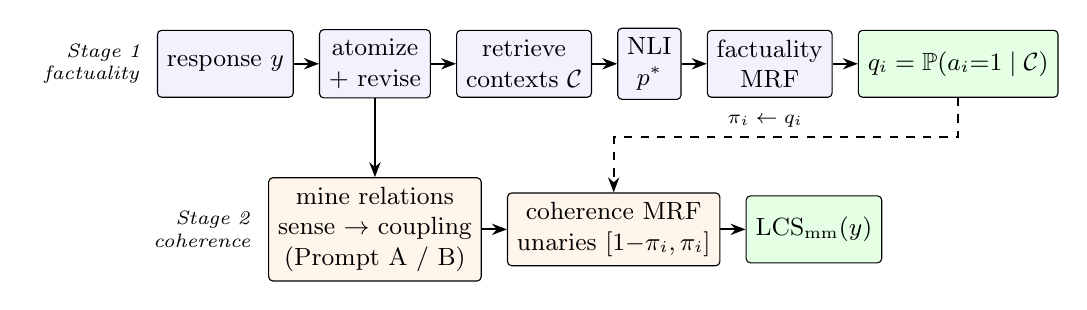
\begin{tikzpicture}[
    font=\small,
    box/.style={draw,rounded corners=1.5pt,align=center,inner sep=3.4pt,
                minimum height=8.5mm},
    s1/.style={box,fill=blue!5},
    s2/.style={box,fill=orange!8},
    fin/.style={box,fill=green!10},
    ar/.style={-{Stealth[length=1.9mm]},thick},
    node distance=3.2mm]

  \node[s1] (resp) {response $y$};
  \node[s1,right=of resp] (atom) {atomize\\+ revise};
  \node[s1,right=of atom] (ret)  {retrieve\\contexts $\mathcal{C}$};
  \node[s1,right=of ret]  (nli)  {NLI\\$p^\ast$};
  \node[s1,right=of nli]  (fmrf) {factuality\\MRF};
  \node[fin,right=of fmrf] (post) {$q_i=\pr{a_i{=}1\mid\mathcal{C}}$};

  \draw[ar] (resp) -- (atom);
  \draw[ar] (atom) -- (ret);
  \draw[ar] (ret)  -- (nli);
  \draw[ar] (nli)  -- (fmrf);
  \draw[ar] (fmrf) -- (post);

  % Mining emits the coupling, so there is no separate compile box.
  \node[s2,below=10mm of atom] (mine)
       {mine relations\\sense $\to$ coupling\\(Prompt A / B)};
  \node[s2,right=of mine] (cmrf)
       {coherence MRF\\unaries $[1{-}\pi_i,\pi_i]$};
  \node[fin,right=of cmrf] (lcs) {$\LCS_{\mm}(y)$};

  \draw[ar] (atom.south) -- ++(0,-4mm) -| (mine.north);
  \draw[ar] (mine) -- (cmrf);
  \draw[ar] (cmrf) -- (lcs);
  \draw[ar,dashed] (post.south) -- ++(0,-5mm) -| (cmrf.north)
        node[pos=0.28,above,font=\scriptsize]{$\pi_i \gets q_i$};

  \node[left=1mm of mine,font=\scriptsize\itshape,align=right,text width=13mm]
       {Stage 2\\coherence};
  \node[left=1mm of resp,font=\scriptsize\itshape,align=right,text width=13mm,
        yshift=0mm] {Stage 1\\factuality};
\end{tikzpicture}}
% scripts/make_pipeline_png.sh defines \plnocaption to render this figure for
% standalone export, where surrounding prose supplies the explanation. Undefined
% in the paper, so the caption below is typeset normally there.
\ifdefined\plnocaption\else
\caption{The two-stage pipeline. Stage 1 (\S\ref{sec-factuality}) is FactReasoner
  \citep{factreasoner}: it grounds each atom against retrieved evidence and returns a
  posterior marginal $q_i$. Stage 2 (\S\ref{sec-coherence}) builds a second MRF over
  the atoms \emph{alone} and adds one pairwise factor per mined atom--atom relation;
  the mined relation already carries its Level-1 coupling, so no separate compile step
  intervenes. The dashed arrow is the only coupling between the stages, and carries
  the composition $\pi_i\!\gets\!q_i$ into the $\phi_i=[1-\pi_i,\pi_i]$ of
  Def.~\ref{def-mrf}. Atomization is shared, so the response is decomposed once and
  both stages score the same claim set; setting $\pi_i\!\equiv\!\tfrac12$ instead
  recovers a pure coherence score that consults no external evidence
  (Rem.~\ref{rem-noevidence}).}
\label{fig:pipeline}
\fi
\end{figure}


\paragraph{The pipeline in one pass.} Figure~\ref{fig:pipeline} is the whole measure, and reading it
left to right fixes what each stage owns. A response $y$ is atomized \emph{once}, into the claim set
both stages then share. Stage~1 takes that set outward: it retrieves evidence $\mathcal{C}$ for each
claim, labels claim--evidence and evidence--evidence pairs by NLI, and runs inference over a factor
graph of claim \emph{and} evidence variables, returning a posterior $q_i=\pr{a_i{=}1\mid\mathcal{C}}$
per claim. Stage~2 takes the same set inward: it mines relations \emph{between} claims from the
response text --- each arriving already typed by an inferential coupling, so nothing intervenes
between mining and model construction --- and builds a second MRF over the claims alone, one pairwise
factor per relation. The two stages meet at exactly one place, the dashed arrow: Stage~1's posterior
becomes Stage~2's prior, $\pi_i\!\gets\!q_i$, occupying the free $\phi_i$ slot of
Def.~\ref{def-mrf}. Everything else runs one way.

That single point of contact is what buys the properties we rely on later. Because atomization is
shared, a factuality verdict and a coherence verdict are statements about the same objects, and the
composition is a substitution into an existing slot rather than a new model
(\S\ref{sec-twostage}). Because the coupling is only the priors, the axes stay separable in both
directions: Stage~1 remains independently reportable, and setting $\pi_i\equiv\tfrac12$ recovers a
coherence score that consults no evidence at all (Rem.~\ref{rem-noevidence}) --- which is the
condition under which every evidence-free comparison of \S\ref{sec-experiments} is run. And because
priors are applied when the network is scored rather than by mutating the mined graph, one mined
graph can be rescored under uniform, factuality-derived or ablated priors without re-running the
estimator, making the prior ablations essentially free.

The coherence model consumes claim-level probabilities and reuses the inference machinery that
produces them, so we describe that stage before defining the model itself. It is FactReasoner
\citep{factreasoner}; the account here is a summary sufficient to make the composition of
\S\ref{sec-twostage} precise, and it also fixes notation and states the estimator whose
label-span construction the relation miner reuses in \S\ref{sec-mining}.

\subsection{Decomposition, retrieval, and relation extraction}

A response $y$ is decomposed by an LLM \emph{atomizer} into atomic claims
$\mathcal{A}=\{a_1,\dots,a_n\}$, each a single independently verifiable proposition. A
\emph{reviser} then decontextualizes each one, resolving pronouns and anaphora so that the claim
is checkable outside its original sentence; near-duplicates are collapsed. For each claim a
retriever returns supporting passages, which are deduplicated into an evidence set
$\mathcal{C}=\{c_1,\dots,c_m\}$.

An LLM-based NLI extractor then labels admitted pairs. For a claim--evidence pair the label is
drawn from $\{\text{entailment},\text{contradiction},\text{neutral}\}$; for an evidence--evidence
pair both directions are scored and reconciled, with entailment in both directions relabelled
\emph{equivalence}. Neutral verdicts are dropped rather than encoded: a claim about which the
evidence is silent contributes no factor and is left at its prior, which is what makes the factor
set of \S\ref{sec-coherence} contain only the relations someone actually asserted.

\subsection{Reading a probability off the generation}
\label{sec-pstar}

Each retained relation carries a probability $p^\ast$. Rather than asking the model to verbalize a
confidence, we read it from the distribution over the tokens it actually emitted. The extractor is
prompted to end with a bracketed label; let $T$ be the set of generated tokens overlapping the
span of that label in the decoded text. Then
\begin{equation}
p^\ast \;=\; \exp\!\Big(\tfrac{1}{|T|}\textstyle\sum_{t\in T}\log p_t\Big),
\label{eq-pstar}
\end{equation}
the per-token geometric-mean probability of the label the model produced. Three details of this
construction are load-bearing, and we record them because each was a source of silent error.

\emph{Span alignment.} The probability is measured over exactly the span the label \emph{parser}
reports, reconstructing the decoded string from the token list and tracking each token's character
offsets. Measuring the same span the label came from makes the label and its probability
structurally unable to disagree. Requiring standalone bracket-delimiter tokens instead does not
work: tokenizers routinely fuse \texttt{[}, \texttt{]} and \texttt{"} into subwords with adjacent
characters, so a delimiter-based rule silently fails on some backends and not others.

\emph{Token-array conventions.} An earlier version of this code stripped the final entry of the
logprob array as an end-of-sequence token. OpenAI-compatible and vLLM logprob arrays contain only
emitted content tokens --- the stop is signalled out of band --- so dropping the last entry
deleted a real content token, and for a bracketed label that token is the one closing the label
whose confidence is being measured.

\emph{Degenerate cases.} When the logprob array is empty, no label span is found, or no token
aligns to it, the estimator returns $0.5$ rather than $0.0$. Returning zero would be read
downstream as a \emph{degenerate, impossible} relation for a label the model in fact generated,
which is a stronger claim than ``we could not measure the confidence''.

\emph{Backends without logprobs.} Some serving stacks expose no token logprobs at all. There
$p^\ast$ instead comes from SIMBA-UQ \citep{simbauq}, which samples the extractor repeatedly across
a temperature schedule, builds a pairwise similarity matrix over the samples, and aggregates each
sample's similarity row into a self-consistency confidence. The winning sample supplies the label
and its aggregated confidence supplies $p^\ast$, so the downstream model is unchanged.

\subsection{The factuality network and its variants}

The labelled graph becomes a pairwise MRF with one binary variable per claim and per evidence
passage. Unary factors are $\phi_X(x)=[1-\pi_X,\;\pi_X]$ with $\pi_X$ the prior on $X$; each
retained relation contributes one pairwise factor from Table~\ref{tab:factors} below, oriented so
the evidence passage is the premise. Marginals $\pr{A_i{=}1}$ are computed by weighted mini-bucket
elimination \citep{wmb} with i-bound $6$, and a claim is reported supported when
$\pr{A_i{=}1}>\tfrac12$.

Three graph variants differ in which factors are admitted: \textsc{fr1} connects each claim only
to the passages retrieved for it; \textsc{fr2} deduplicates passages and scores every claim
against all of them; \textsc{fr3} adds evidence--evidence factors. We use \textsc{fr2}. Because
scoring every claim against every passage is $O(nm)$ LLM calls, a candidate-pair policy can restrict
the pairs actually scored; the calibration of that policy is instructive for the analogous choice
in \S\ref{sec-mining}. Replaying policies against recorded verdicts on a 20-claim narrative with 60
passages, a provenance-restricted policy with an embedding similarity gate holds recall at $1.000$
through a threshold of $0.20$, slipping to $0.985$ at $0.30$ and $0.833$ at $0.40$. Substituting
token-Jaccard similarity for sentence embeddings, however, loses $22$ of $72$ non-neutral relations
and moves the factuality score by $0.05$ --- and \emph{no} threshold recovers full recall, even
$0.05$. Cheap surrogates for semantic similarity are not safe here, and the saving is
workload-dependent rather than constant: roughly $5\times$ on unrelated subtopics but $1.2\times$
on a narrative where every claim shares characters.

\paragraph{Conventions.} We use the with-priors factor tables (Table~\ref{tab:factors}) throughout,
with $\pi_C=0.9$ for evidence and $\pi_A=0.5$ for claims. The published factuality model uses the
no-priors tables and a higher evidence prior. The difference is immaterial to the coherence results
below, which set claim priors explicitly, but the convention must be stated because the two table
families are not interchangeable --- that is the subject of \S\ref{sec-potentials}.

%% ================================================================
\section{Stage two: the coherence Markov random field}
\label{sec-coherence}
%% ================================================================

\subsection{The model}
\label{sec-model}

\begin{definition}[Coherence MRF]
\label{def-mrf}
Let $\mathcal{A}=\langle a_1,\dots,a_n\rangle$ be the atomic claims of a response in assertion
order, each a binary variable with $a_i=1$ read as ``the claim holds''. Let
$\mathcal{R}=\{(s_r,t_r,\tau_r,p_r)\}_{r=1}^{|\mathcal{R}|}$ be a set of \emph{relations}, where
$s_r\neq t_r$ index claims, $\tau_r$ is an inferential coupling (Def.~\ref{def-couplings}), and
$p_r\in[0,1]$ is the relation's weight. Given priors $\pi\in[0,1]^n$, the coherence MRF induced by
$(\mathcal{A},\mathcal{R},\pi)$ is
\begin{equation}
\pr{\mathbf{a}} \;=\; \frac{1}{Z}\;
  \prod_{i=1}^{n}\phi_i(a_i)\;
  \prod_{r\in\mathcal{R}}\psi_{\tau_r,p_r}\!\left(a_{s_r},a_{t_r}\right),
\qquad
Z \;=\; \sum_{\mathbf{a}\in\{0,1\}^n}\;\prod_{i}\phi_i(a_i)\prod_{r}\psi_r ,
\label{eq-joint}
\end{equation}
where $\phi_i(a_i)=[1-\pi_i,\;\pi_i]$ over the states $(0,1)$ and $\psi_{\tau,p}$ is given by
Table~\ref{tab:factors}.
\end{definition}

Three structural properties of Definition~\ref{def-mrf} deserve statement, because each is a
deliberate commitment rather than an implementation detail.

\begin{remark}[The factor family is closed]
\label{rem-closed}
A coupling is nothing more than a choice of which cells of a $2\times2$ table are down-weighted
and by how much. Every $\psi_{\tau,p}$ in Table~\ref{tab:factors} is determined by $p$, the source
prior $\pi_s$, and the penalized set; the whole inferential vocabulary is therefore a
three-parameter pairwise family. This is a guarantee about what the model \emph{cannot} do: no
relation type, however elaborately named at the discourse level, can smuggle in expressiveness
beyond a pairwise potential. Appendix~\ref{app-mln} contrasts this with Markov logic, whose rule
vocabulary is open by design.
\end{remark}

\begin{remark}[Order-sensitivity enters only through the relations]
\label{rem-order}
Nothing in Eq.~\ref{eq-joint} references claim position. Assertion order enters exclusively
through \emph{which} pairs are related and in \emph{which} direction. It follows that an edit which
preserves the relation set --- reordering claims whose relations are symmetric, or exchanging a
temporal \sense{Precedence} for a \sense{Succession}, which Table~\ref{tab:compile} maps to no
factor at all --- provably cannot change any readout. This is a falsifiable prediction about the
measure and not merely a design note; \S\ref{sec-locobench} describes the ladder built to test it.
\end{remark}

\begin{remark}[Coherence is evaluated without evidence]
\label{rem-noevidence}
The graph of Definition~\ref{def-mrf} contains claim variables only. No retrieved passage appears,
and with uniform priors $\pi_i\equiv\tfrac12$ the model consults no external knowledge whatever: it
scores how the response hangs together, not whether it is true. This is what makes the two axes
separable, and \S\ref{sec-twostage} shows how to couple them when a joint reading is wanted.
\end{remark}

\subsection{Level one: inferential couplings}
\label{sec-couplings}

\begin{definition}[Inferential couplings]
\label{def-couplings}
A coupling $\tau$ is specified by the set $V(\tau)\subseteq\{0,1\}^2$ of joint assignments
$(a_s,a_t)$ it \emph{penalizes} --- equivalently, the configurations at which the relation is
violated. The vocabulary is:
\begin{center}\small
\begin{tabular}{@{}llcl@{}}
\toprule
Coupling & Reading & Directed & Penalized set $V(\tau)$ \\
\midrule
\ent            & $a_s \Rightarrow a_t$              & yes & $\{(1,0)\}$ \\
\con            & $a_s \Rightarrow \neg a_t$         & yes & $\{(1,1)\}$ \\
\eqv            & $a_s \Leftrightarrow a_t$          & no  & $\{(0,1),(1,0)\}$ \\
\exc            & exactly one of $a_s,a_t$ holds     & no  & $\{(0,0),(1,1)\}$ \\
\cnc            & at least one of $a_s,a_t$ holds    & no  & $\{(0,0)\}$ \\
\coupling{none} & no coupling                        & ---  & $\varnothing$ (no factor) \\
\bottomrule
\end{tabular}
\end{center}
Write $\mathcal{T}$ for the five edge-producing couplings and
$\mathcal{T}_{\mathrm{conf}}=\{\con,\exc\}$ for the \emph{conflict} couplings, those whose
penalized set contains the both-true world $(1,1)$.
\end{definition}

\begin{table}[tp]
\centering\footnotesize
\setlength{\tabcolsep}{4pt}
\renewcommand{\arraystretch}{1.15}
\caption{One realistic response excerpt per Level-1 coupling of Def.~\ref{def-couplings}. As in
  Table~\ref{tab:senseex}, each excerpt is prose containing both claims --- \uline{$A$ is the
  source, underlined}, \textbf{$B$ the target, bold}, the \emph{italic} words drawing the link ---
  and $V(\tau)$ is repeated from Def.~\ref{def-couplings} so the excerpt can be read against the
  world it rules out. The \emph{Why} column names the world the response denies, which is what
  distinguishes each coupling from the one above it; the three conflict-adjacent couplings \con{},
  \exc{} and \cnc{} are illustrated on one two-part weld failure so that only exhaustiveness
  varies. \coupling{none} produces no factor, so its excerpt is one where the text relates the
  claims without constraining their truth.}
\label{tab:coupex}
\begin{tabularx}{\textwidth}{@{}l l l X@{}}
\toprule
Coupling & Reading & $V(\tau)$ & Response excerpt, and the world it denies \\
\midrule
\ent & $a_s\Rightarrow a_t$ & $\{(1,0)\}$
  & ``\uline{The alloy is chemically identical to the certified reference}, \emph{and therefore}
    \textbf{it meets the airframe specification}.''
    \newline\emph{Why:} the response rules out the world where the source holds and the target
    fails --- $(1,0)$ --- and says nothing about the case where the alloy differs, which is why
    the $a_s{=}0$ row returns the target to its prior. \\
\midrule
\con & $a_s\Rightarrow\neg a_t$ & $\{(1,1)\}$
  & ``\uline{The weld passed the tensile test}, \emph{yet} \textbf{the same joint was porous along
    its full length}.''
    \newline\emph{Why:} only the both-true world $(1,1)$ is denied. Both can still fail together
    --- if the wrong joint was tested, neither claim holds --- so $(0,0)$ must stay available. \\
\midrule
\exc & exactly one holds & $\{(0,0),(1,1)\}$
  & ``The joint was destructively examined, so \emph{exactly one of} \uline{the weld met the
    tensile minimum} \emph{and} \textbf{the weld fell short of it} \emph{must be the finding} ---
    \emph{there is no third outcome}.''
    \newline\emph{Why:} both same-value worlds are denied. The added $(0,0)$ is the whole
    difference from \con{}: once the joint has actually been examined the pair cannot both fail,
    so leaving that world open --- as \con{} does --- would under-penalize the conflict. \\
\midrule
\cnc & at least one holds & $\{(0,0)\}$
  & ``The fracture began at the joint, so \emph{at least one of} \uline{the weld} \emph{and}
    \textbf{the fastener} \emph{must have given way} --- conceivably both.''
    \newline\emph{Why:} the dual of \exc{}. Only the both-false world is denied, so asserting the
    disjunction is evidence \emph{for} both endpoints (Example~\ref{ex-cnc}). \\
\midrule
\eqv & $a_s\Leftrightarrow a_t$ & $\{(0,1),(1,0)\}$
  & ``\uline{The shipment was certified to specification} --- \emph{that is to say},
    \textbf{every contractual requirement had been met}.''
    \newline\emph{Why:} the two disagreeing worlds are denied, in both directions; unlike \ent{}
    there is no vacuous row, since a false source now also forces a false target. \\
\midrule
\coupling{none} & no coupling & $\varnothing$
  & ``\uline{The replacement units were installed in March}, \emph{some three months before}
    \textbf{the first in-flight failures were reported}.''
    \newline\emph{Why:} no world is denied. The response genuinely relates the claims, but
    ordering them in time constrains neither one's truth, so the pair contributes
    \textbf{no factor} and both claims stay at their priors. \\
\bottomrule
\end{tabularx}
\end{table}

Table~\ref{tab:coupex} gives a response excerpt for each coupling, set against the world that
coupling denies; since a coupling \emph{is} its penalized set, reading the two together is the
quickest way to see what each one commits the response to. The first three couplings are exactly
the NLI edge types of \S\ref{sec-factuality}, which is what lets a mined relation reuse the
existing graph machinery unchanged. The last two are additions required by argumentative prose,
and the distinction between them and \con{} is the one the taxonomy exists to draw.

\paragraph{Why exhaustiveness needs its own coupling.} \con{} forbids only the both-true world: two
claims that cannot both hold, but might both fail. \exc{} additionally forbids the both-false
world, which is what \emph{exhaustive} alternatives assert. ``No one was harmed'' and ``three
people died'' can neither both hold nor both fail --- either someone was harmed or no one was ---
so a model that treats them as mere opposition has mis-described the situation in a way that
matters for scoring: it leaves available a world in which \emph{neither} claim is true, and so
under-penalizes. Conversely \cnc{} is the dual, penalizing only the both-false world, and is what a
disjunction asserts (``at least one of these two findings must hold''). Adjudicated disputes ---
incident investigations, litigation, competing hypotheses --- are precisely the domains where
exhaustive pairs occur, because the function of a finding is to close one. The \con{}, \exc{} and
\cnc{} rows of Table~\ref{tab:coupex} state one two-part weld failure three times over, so that
the only thing varying across them is which same-value worlds the response leaves standing.

\begin{example}[A \cnc{} factor in isolation]
\label{ex-cnc}
Take a single \cnc{} relation with $p=0.9$ over two claims with priors $\pi=0.5$, and no other
factors. From Table~\ref{tab:factors} the pairwise table is $[1-p,\;\pi_s,\;\pi_s,\;p]
=[0.1,0.5,0.5,0.9]$, and multiplying in the unaries and normalizing gives world masses
\[
\pr{0,0}=0.05,\quad \pr{0,1}=0.25,\quad \pr{1,0}=0.25,\quad \pr{1,1}=0.45 .
\]
The both-false world is suppressed from the $0.25$ it would receive under independent fair priors
to $0.05$, while the three worlds satisfying ``at least one holds'' share the recovered mass in
proportion to how many endpoints they assert. Each marginal rises from $0.5$ to $0.7$: asserting
that at least one of two claims holds is evidence for both, which is the intended reading.
\end{example}

\subsection{The pairwise potentials, and why factuality's tables are wrong here}
\label{sec-potentials}

\begin{table}[t]
\centering\small
\caption{Pairwise potentials $\psi_{\tau,p}(a_s,a_t)$, listed row-major over the assignments
  $(0,0),(0,1),(1,0),(1,1)$; $\pi_s$ is the source claim's prior and bold marks the penalized set
  $V(\tau)$ of Def.~\ref{def-couplings}. The \emph{no-priors} family is correct for
  claim--evidence factuality, where the source passage's own truth is at stake; the
  \emph{with-priors} family is what coherence requires (Prop.~\ref{prop-rowstoch}) and what
  Def.~\ref{def-mrf} uses. The two symmetric couplings \eqv{} and \exc{} coincide in both
  families, having no source-prior term to correct.}
\label{tab:factors}
\begin{tabular}{@{}llll@{}}
\toprule
Coupling $\tau$ & No priors & With priors & Symmetry \\
\midrule
\ent  & $[p,\;p,\;\mathbf{1\!-\!p},\;p]$
      & $[1\!-\!\pi_s,\;\pi_s,\;\mathbf{1\!-\!p},\;p]$ & asymmetric \\
\con  & $[p,\;p,\;p,\;\mathbf{1\!-\!p}]$
      & $[1\!-\!\pi_s,\;\pi_s,\;p,\;\mathbf{1\!-\!p}]$ & asymmetric \\
\eqv  & \multicolumn{2}{l}{$[p,\;\mathbf{1\!-\!p},\;\mathbf{1\!-\!p},\;p]$} & symmetric \\
\exc  & \multicolumn{2}{l}{$[\mathbf{1\!-\!p},\;p,\;p,\;\mathbf{1\!-\!p}]$} & symmetric \\
\cnc  & $[\mathbf{1\!-\!p},\;p,\;p,\;p]$
      & $[\mathbf{1\!-\!p},\;\pi_s,\;\pi_s,\;p]$ & symmetric \\
\bottomrule
\end{tabular}
\end{table}

\begin{proposition}[Row-stochasticity of the asymmetric couplings]
\label{prop-rowstoch}
The with-priors tables of the two \emph{asymmetric} couplings are row-stochastic in the source
state: for $\tau\in\{\ent,\con\}$ each row of $\psi_{\tau,p}$ sums to one, so the row indexed by
$a_s$ \emph{is} the conditional distribution $\pr{a_t \mid a_s}$, with
\[
\pr{a_t{=}1 \mid a_s{=}0} = \pi_s, \qquad
\pr{a_t{=}1 \mid a_s{=}1} = \begin{cases}
p & \tau=\ent\\ 1-p & \tau=\con .
\end{cases}
\]
Consequently such a factor constrains the target only when the source is true; when the source is
false it returns the target to the prior. The symmetric couplings are not of this form, and are not
claimed to be. In particular
$\cnc$ is \emph{not} row-stochastic: its rows sum to $(1-p)+\pi_s$ and $\pi_s+p$, which both equal
one only in the degenerate case $p=\pi_s=\tfrac12$.
\end{proposition}

\begin{proof}
For both asymmetric tables the $a_s{=}0$ row is $[1-\pi_s,\;\pi_s]$, which sums to one; the
$a_s{=}1$ row is $[1-p,\;p]$ for \ent{} and $[p,\;1-p]$ for \con{}, each summing to one. Dividing a
row by its sum is therefore the identity, so the rows already are conditionals and may be read off
directly. For \cnc{} $=[1-p,\;\pi_s,\;\pi_s,\;p]$, row-stochasticity would require
$(1-p)+\pi_s=1$ and $\pi_s+p=1$, i.e.\ $\pi_s=p$ and $\pi_s=1-p$ simultaneously, hence $p=1-p$.
\end{proof}

\paragraph{What row-stochasticity means, and what it does not.} The condition is a statement about
the \emph{table}: it says each row of $\psi$, read across the target's two states, is already
normalized, so $\psi(a_s,\cdot)$ can be read as $\pr{a_t\mid a_s}$ rather than as an unnormalized
compatibility score. Two consequences follow, and a third does not. First, the $a_s{=}0$ row being
the prior $[1-\pi_s,\pi_s]$ is what makes a false source \emph{uninformative} about the target,
which is the formal content of ``an implication says nothing when its antecedent fails''. Second,
writing $\ln\psi = \alpha+\beta a_s+\gamma a_t+\delta\,a_s a_t$, row-stochasticity \emph{pins} the
source-only weight: $\beta=\ln\frac{1-p}{1-\pi_s}$ for \ent{}, with the other couplings tabulated in
App.~\ref{app-mln}. The source term is not zero, but neither is it free --- it is exactly the amount
needed to hold the $a_s{=}0$ row at the prior, so no residual degree of freedom is left with which
the relation could bid the source's own plausibility up or down. That is what distinguishes these
tables from the no-priors family below, whose $(0,\cdot)$ row is $[p,p]$ and so trades the source's
truth against the target's. What does \emph{not} follow is any invariance of the marginals in the assembled
model: once a factor is multiplied against its neighbours and renormalized, both endpoints can
move, and for an isolated \ent{} relation the source's own marginal already departs from $\pi_s$
whenever $\pi_t\neq\tfrac12$. Row-stochasticity constrains how a relation \emph{enters} the joint,
not where inference then lands.

\begin{table}[htbp]
\centering\small
\caption{Proposition~\ref{prop-rowstoch} made concrete, at $p=0.9$ and $\pi_s=0.5$ so the three
  couplings are directly comparable. Tables are row-major over $(0,0),(0,1),(1,0),(1,1)$, so the
  first pair is the $a_s{=}0$ row and the second the $a_s{=}1$ row. The two asymmetric couplings
  have both rows summing to one and so admit the conditional reading; \cnc{} does not, and its
  rows are the entry marked in bold. Every value is produced by
  \texttt{fact\_reasoner.factors.edge\_factor\_values}.}
\label{tab:rowstoch-ex}
\begin{tabular}{@{}llccccl@{}}
\toprule
$\tau$ & Table & \multicolumn{2}{c}{Row sums} & \multicolumn{2}{c}{Conditional reading} & \\
\cmidrule(r){3-4}\cmidrule(r){5-6}
 & & $a_s{=}0$ & $a_s{=}1$ & $\pr{a_t{=}1|a_s{=}0}$ & $\pr{a_t{=}1|a_s{=}1}$ & Reading \\
\midrule
\ent & $[.5,\,.5,\,.1,\,.9]$ & $1.0$ & $1.0$ & $0.5=\pi_s$ & $0.9=p$
  & source true $\Rightarrow$ target up \\
\con & $[.5,\,.5,\,.9,\,.1]$ & $1.0$ & $1.0$ & $0.5=\pi_s$ & $0.1=1\!-\!p$
  & source true $\Rightarrow$ target down \\
\cnc & $[.1,\,.5,\,.5,\,.9]$ & $\mathbf{0.6}$ & $\mathbf{1.4}$ & $0.833$ & $0.643$
  & source \emph{false} $\Rightarrow$ target up \\
\bottomrule
\end{tabular}
\end{table}

Table~\ref{tab:rowstoch-ex} states the proposition in numbers, and the three rows are worth reading
against the prose they encode. For \ent{} --- ``Voyager~1 crossed the heliopause, so its
instruments measured the density rise'' --- a true source pulls the target up to $p=0.9$, while a
false source leaves it at the $0.5$ prior: the row is flat, which is exactly a vacuous antecedent.
For \con{} --- ``the probe is in interstellar space, so it has \emph{not} left the Solar System''
--- a true source pushes the target down to $1-p=0.1$, and a false source is again silent. Both
rows normalize, so both readings are conditional probabilities.

\cnc{} inverts the direction of information and thereby breaks the property. Reading the weld
example of Table~\ref{tab:coupex} --- ``at least one of the weld and the fastener must have given
way'' --- it is the weld \emph{holding} that forces the fastener to have failed, so the
informative row is $a_s{=}0$, where the reading is $0.833$, well above the $0.5$ prior. The
$a_s{=}1$ row is the weak one: once the weld has failed the disjunction is already satisfied and
the fastener is left near its prior. A source-conditioned normalization cannot express this, since
it reserves the flat row for the false source; the rows sum to $0.6$ and $1.4$ instead of to one.
This is not a defect of the \cnc{} table but a property of disjunction, and Example~\ref{ex-cnc}
shows the same fact from the joint side: both endpoints rise together, from $0.5$ to $0.7$,
because the factor is symmetric and pushes neither endpoint preferentially.

Proposition~\ref{prop-rowstoch} is the substantive modelling choice of this section, and the
contrast with the no-priors family is worth being precise about. In the no-priors \ent{} table the
$(1,0)$ cell is $1-p$ \emph{and the $(0,\cdot)$ cells are both $p$}, so the table charges the
\emph{source} being true whenever the target is uncertain. That is appropriate for
claim--evidence factuality: there the source is a retrieved passage whose own reliability is in
question, and an entailment from a passage to a claim the model doubts is evidence against the
passage. It is wrong for coherence, where the source is another claim of the same response, and
where a well-supported premise must not be penalized for being a premise.

The consequence is not a matter of degree. On the response of \S\ref{sec-example-aero} --- sixteen
claims joined by a twelve-edge entailment backbone --- the no-priors tables drive the root of the
backbone to $\pr{a_1{=}1}=0.19$, far below its $0.5$ prior, purely because it is the premise of a
chain whose later members are uncertain. The mean marginal sits at $0.490$ and moves only to
$0.498$ when every conflict edge is deleted, a range of $0.008$. Under the with-priors tables the
same comparison runs $0.607$ to $0.620$: a range more than $1.5$ times larger, from a base that is
not already depressed by the backbone itself. All four values are exact, by $2^{16}$ enumeration. A
coherence measure built on the factuality tables does not merely give different numbers; it spends
its dynamic range penalizing premises and has little left for conflicts, which are the thing being
measured.

\subsection{Level two: discourse senses and the compile map}
\label{sec-level2}

Couplings are the right vocabulary for a factor table and the wrong one for annotation. Asked
whether two claims stand in \ent{}, an annotator --- human or model --- has been handed a question
about logic, when the fact actually observable in the text is a question about discourse: does this
sentence give a cause, offer evidence, concede a tension, or lay out alternatives? We therefore
mine an interpretable layer and compile it down.

\begin{definition}[Compile map]
\label{def-compile}
Let $\mathcal{S}$ be the set of Level-2 discourse senses. The compile map
\[
\mathcal{C}:\;\mathcal{S}\;\longrightarrow\;
  \bigl(\mathcal{T}\cup\{\coupling{none}\}\bigr)\times\bigl([0,1]\cup\{\bot\}\bigr)\times\{0,1\}^3
\]
assigns to each sense a coupling, a strength prior ($\bot$ meaning ``use the estimator's own
value''), and the flags \emph{directed}, \emph{concession} and \emph{ordering-only}. It is total,
deterministic, and given in Table~\ref{tab:compile}.
\end{definition}

\begin{table}[t]
\centering\small
\caption{The compile map $\mathcal{C}$ of Def.~\ref{def-compile}. \emph{Ordering-only} senses
  record assertion order but induce \textbf{no factor}, which is what makes an order-only edit
  provably score-invariant (Rem.~\ref{rem-order}). \sense{Concession} is a conflict the text may
  itself resolve, handled by Eq.~\ref{eq-concession}. The nine senses marked $\star$ form the
  admissible vocabulary of \S\ref{sec-mining}.}
\label{tab:compile}
\begin{tabular}{@{}llccll@{}}
\toprule
Level-2 sense & $\mathcal{C}$ coupling & prior & dir. & flag & gloss \\
\midrule
\sense{Cause-Effect}$^\star$   & \ent & $\bot$ & yes & & source brings target about \\
\sense{Effect-Cause}$^\star$   & \ent & $\bot$ & yes & & source is the effect, target the cause \\
\sense{Evidence}$^\star$       & \ent & $\bot$ & yes & & source is evidence for target \\
\sense{Condition}              & \ent & $\bot$ & yes & & source conditions target \\
\sense{Instantiation}          & \ent & $\bot$ & yes & & target instantiates source \\
\sense{Restatement}$^\star$    & \eqv & $0.90$ & no  & & definitional identity \\
\sense{Contrast}$^\star$       & \con & $\bot$ & no  & & opposed, \emph{not} exhaustive \\
\sense{Concession}$^\star$     & \con & $\bot$ & yes & conc. & a tension the text resolves \\
\sense{Alternative}$^\star$    & \exc & $\bot$ & no  & & exhaustive: exactly one holds \\
\sense{Disjunction}$^\star$    & \cnc & $\bot$ & no  & & at least one holds \\
\sense{Precedence}$^\star$     & \coupling{none} & --- & yes & ord. & temporal order only \\
\sense{Succession}             & \coupling{none} & --- & yes & ord. & temporal order only \\
\bottomrule
\end{tabular}
\end{table}

\begin{table}[tp]
\centering\footnotesize
\setlength{\tabcolsep}{4pt}
\renewcommand{\arraystretch}{1.15}
\caption{One realistic response excerpt per Level-2 sense of Table~\ref{tab:compile}, in the same
  row order and grouped by the coupling each compiles to. Each excerpt is prose of the kind the
  estimator actually sees and \emph{contains both claims}: \uline{$A$ is underlined}, \textbf{$B$ is
  bold}, and the \emph{italic} words are the ones that draw the link --- the span
  \S\ref{sec-mining} obliges the model to quote, which is why it must be findable in the response
  and not in either claim. Senses are marked $\star$ when admissible; the three unmarked ones are
  included because their breadth is the argument for excluding them (\S\ref{sec-mining}). The
  \sense{Contrast}, \sense{Alternative} and \sense{Disjunction} rows describe one two-part weld
  failure three ways, separated only by exhaustiveness (\S\ref{sec-couplings}); they reuse the
  scenario of Table~\ref{tab:coupex} deliberately, so that a discourse sense and the coupling it
  compiles to can be compared on the same prose.}
\label{tab:senseex}
\begin{tabularx}{\textwidth}{@{}llX@{}}
\toprule
Level-2 sense & $\mathcal{C}$ & Response excerpt, and why this sense rather than a neighbour \\
\midrule
\sense{Cause-Effect}$^\star$ & \ent
  & ``\uline{The company shipped a batch it knew to be out of tolerance}, and \emph{as a direct
    result} \textbf{its share price fell $15\%$ that quarter}.''
    \newline\emph{Why:} the response itself presents $A$ as bringing $B$ about; the marker names the
    direction. \\
\sense{Effect-Cause}$^\star$ & \ent
  & ``\uline{The entire fleet was grounded on 14 March}. The order came \emph{because}
    \textbf{inspectors had found a cracked wing spar on two airframes}.''
    \newline\emph{Why:} the same support runs from the stated effect to its cause. Direction of
    \emph{explanation} is reversed; direction of inferential support is not. \\
\sense{Evidence}$^\star$ & \ent
  & ``\uline{The maintenance log records no inspection between January and June}, \emph{which
    shows that} \textbf{the mandatory 500-hour check was skipped}.''
    \newline\emph{Why:} $A$ is offered in support of $B$ without any claim that it caused it ---
    a record is evidence, not a mechanism. \\
\sense{Condition} & \ent
  & ``\textbf{A part is cleared for airframe use} \emph{only if} \uline{its alloy meets the
    reference specification}.''
    \newline\emph{Why:} $B$ is asserted contingent on $A$. Note how weakly the cue constrains:
    nearly any dependence can be reread as a condition, which is why the sense is inadmissible. \\
\sense{Instantiation} & \ent
  & ``\uline{Several suppliers failed the 2023 audit} --- \emph{for instance},
    \textbf{the Tucson plant failed on two counts}.''
    \newline\emph{Why:} $B$ is one case falling under $A$'s generalization. Like
    \sense{Condition}, broad enough to fit almost any pair that shares a topic. \\
\midrule
\sense{Restatement}$^\star$ & \eqv
  & ``\uline{The shipment was certified to specification} --- \emph{in other words},
    \textbf{every requirement in the contract had been met}.''
    \newline\emph{Why:} a \emph{marked} paraphrase asserts identity of content, which is why the
    strength prior is fixed at $0.90$ rather than estimated. \\
\midrule
\sense{Contrast}$^\star$ & \con
  & ``\uline{The weld passed the tensile test}, \emph{but} \textbf{the same joint was porous
    along its full length}.''
    \newline\emph{Why:} opposed and \emph{not} exhaustive. A third possibility --- the wrong joint
    was tested --- leaves both false, so the both-false world must stay available. \\
\sense{Concession}$^\star$ & \con
  & ``\emph{Although} \uline{the airline argued throughout that pilot error was to blame},
    \textbf{the final report identified a metallurgical defect}; the tribunal \emph{ultimately
    held} for the latter.''
    \newline\emph{Why:} a tension the text itself settles. The resolving holding triggers the
    discount of Eq.~\ref{eq-concession} rather than counting as a live conflict. \\
\midrule
\sense{Alternative}$^\star$ & \exc
  & ``The two accounts cannot be reconciled: \emph{either} \uline{no one aboard was harmed},
    \emph{or} \textbf{three passengers died}, and \emph{exactly one of them is true}.''
    \newline\emph{Why:} exhaustive. Unlike \sense{Contrast} the pair can neither both hold nor
    both fail, so the both-false world is penalized too. \\
\midrule
\sense{Disjunction}$^\star$ & \cnc
  & ``Metallurgy confirms the fracture began at the joint, so \emph{at least one of}
    \uline{the weld} \emph{and} \textbf{the fastener} \emph{must have failed} --- possibly
    both.''
    \newline\emph{Why:} at least one holds and both may. The dual of \sense{Alternative}:
    only the both-false world is penalized. \\
\midrule
\sense{Precedence}$^\star$ & \coupling{none}
  & ``\uline{The replacement units were installed in March}, \emph{some three months before}
    \textbf{the first in-flight failures were reported in June}.''
    \newline\emph{Why:} the text genuinely relates the two claims, and says nothing about either
    one's truth --- so the sense induces \textbf{no factor}. \\
\sense{Succession} & \coupling{none}
  & ``\textbf{The first in-flight failures were reported in June}, \emph{fully three months
    after} \uline{the replacement units had been installed}.''
    \newline\emph{Why:} the mirror of \sense{Precedence} --- the same two claims, the same
    absence of truth-functional content. Offering both senses invites an arbitrary choice on a
    relation that produces no factor either way. \\
\bottomrule
\end{tabularx}
\end{table}

Table~\ref{tab:senseex} grounds each sense in a response excerpt that contains both claims and
the wording that licenses the link, since what an annotator must actually recognize is a form of
words rather than a truth-functional pattern. Several entries encode judgements worth defending. \sense{Restatement}
carries a fixed strength prior of $0.90$ because a marked paraphrase (``in other words'',
``equivalently'') is a claim about identity of content, and a model asked to estimate its strength
has little to add; the estimator's value is used when available, and the prior seeds it otherwise.
Five senses collapse onto \ent{}, which is a deliberate loss: the model does not distinguish
causation from evidence, because a pairwise potential over truth values cannot. The grouped \ent{}
block of Table~\ref{tab:senseex} shows exactly what compilation discards --- five distinct
discourse facts, one factor table. What survives compilation is the inferential force, and the
sense is retained alongside it for interpretability and for error analysis.

The \sense{Contrast}/\sense{Alternative} boundary is exactly the exhaustiveness question of
\S\ref{sec-couplings}, and the \sense{Contrast}, \sense{Alternative} and \sense{Disjunction} rows of
Table~\ref{tab:senseex} are that question in concrete form: one two-part weld failure written up
three ways --- as mere opposition, as an exhaustive choice, and as a disjunction --- differing in
nothing but which same-value worlds the response leaves available. The two
ordering-only senses are the taxonomy's way of representing a
relation the text genuinely draws while asserting that it has no truth-functional content: a
narrative that says one event preceded another has related the two claims, and has said nothing
about whether either is true.

\paragraph{Concession: a conflict the text resolves.} A \sense{Concession} asserts a tension and
then overrides it. ``The airline argued pilot error, but the final report found a metallurgical
defect'' is not an incoherence if the report's finding is presented as authoritative; treating it
as a live contradiction would penalize a response for doing the very thing careful argument
requires. When a resolving \emph{holding} claim $h$ is present we discount the conflict's weight,
\begin{equation}
p_r^{\mathrm{eff}} \;=\; p_r\,\bigl(1-\lambda\,\pi_h\bigr),
\label{eq-concession}
\end{equation}
with $\lambda=0.45$; absent a resolver the relation stands at full strength and the tension counts
against the response. Holdings are identified by adjudicative cue phrases (\emph{held},
\emph{ruled}, \emph{concluded}, \emph{found that}, \emph{the tribunal}, \emph{ultimately}) on a
claim that is not itself an endpoint of the relation and that maximizes lexical overlap with the
two endpoints. This is a heuristic, and with $\lambda$ it is the one place in the design where
hand-set constants enter; \S\ref{sec-limitations} returns to the point.

\subsection{Estimating relations from the response}
\label{sec-mining}

Definition~\ref{def-mrf} takes $\mathcal{R}$ as given. In use it must be estimated from the text,
and the estimator is the weakest link in the pipeline (\S\ref{sec-experiments}), so we specify it
carefully.

\paragraph{The estimand, decomposed.} A relation's weight factors into a type term and a strength
term:
\begin{equation}
p_r \;=\; \underbrace{\pr{\tau \mid a_s,a_t,y}}_{\text{type confidence}}\;\cdot\;
          \underbrace{\pr{a_t \mid a_s,\tau,y}}_{\text{conditional strength}} .
\label{eq-decomp}
\end{equation}
The first factor asks how confident we are that this is a \emph{$\tau$-relation at all}; the second,
given that it is, how strongly the source determines the target. Conflating them is a mistake: a
confidently-identified weak causal link and a doubtfully-identified strong one are different
epistemic situations that a single elicited number cannot distinguish. Two prompts estimate them
separately (full texts in Appendix~\ref{app-prompts}).

\emph{Prompt A} elicits the discourse sense and its coupling, with chain-of-thought \emph{preceding}
the label so the model commits to a sense only after reasoning --- and so that the label's token
logprobs, read exactly as in Eq.~\ref{eq-pstar}, measure a decision already made rather than one
being made. \emph{Prompt B} elicits the conditional strength as a surrogate token: the answer's first
word must be \texttt{Yes} or \texttt{No}, and the strength is the renormalized
$\pr{\texttt{Yes}}/(\pr{\texttt{Yes}}+\pr{\texttt{No}})$ \citep{kadavath}, or the affirmative
fraction over $N$ samples where logprobs are unavailable. The question is deliberately graded ---
``is the implication at least plausible?'' rather than ``is it certain?'' --- so that a weak but real
link is not forced to answer \texttt{No}; its weakness surfaces in the renormalized probability
instead. A verbalized variant asking for \texttt{[p=0.NN]} directly is retained only as a
comparison, verbalized confidence being weakly calibrated \citep{xiong}.

\paragraph{Grounding is mandatory, not optional.} Prompt A always receives the full response, and is
instructed to assert a coupling only where the response \emph{itself} draws the connection. This is
the single most consequential decision in the estimator. Judging a claim pair in isolation invites
the model to accept any abstractly plausible relation, and the failure is not a mild
over-generation: measured relation density reaches six to nine relations per claim, including
spurious contradictions on paragraphs that contain none. Because Eq.~\ref{eq-joint} is a product
over relations, a graph of many soft mutually-constraining edges drives every marginal toward the
prior, so an over-connected graph does not merely add noise --- it destroys the measure's ability to
distinguish a coherent response from an incoherent one, in the direction of calling everything
mediocre.

Two further precision mechanisms are used, one requested and one checkable. The \emph{admissibility
filter} restricts output to the nine $(\text{sense},\text{coupling})$ combinations marked $\star$ in
Table~\ref{tab:compile}. \sense{Condition} and \sense{Instantiation} are the notable exclusions:
both compile to \ent{} and both are semantically broad --- their rows in
Table~\ref{tab:senseex} illustrate the breadth, since almost any dependence can be read as a
condition and almost any topical pair as an instantiation --- so a model reaching for ``these two
claims are related somehow'' lands on them readily; they accounted for $13\%$ of one measured arm's
edges while appearing zero times in gold. The \emph{evidence-span requirement} obliges the model to
quote, verbatim from the response, the words that draw the link; the parser then verifies that the
quotation is actually a substring of the response and drops the relation otherwise. This is the only
precision mechanism in the estimator that is \emph{checked} rather than merely asked for. It must
quote the response and not the claims, because claims are decontextualized rewrites and only about
$27\%$ of them appear in the response verbatim even after normalization.

\paragraph{Two prompt generations.} The first-generation Prompt A over-asserts badly: against a
corpus in which $7.2\%$ of candidate pairs are genuinely related, it answers ``related'' on $72\%$ of
the pairs a windowed policy hands it. Five properties push it that way, and the revision addresses
each. (i) Its few-shot balance was three related to one unrelated; class balance in the exemplars is
a strong prior on the answer distribution, and this one pointed the wrong way by an order of
magnitude. The revision is two related to three unrelated. (ii) Its single negative exemplar had the
response \emph{explicitly disavow} a link (``the two processes were not related this year''), which
teaches that \coupling{none} requires denial, whereas real prose simply stays silent; the revision's
negatives are all silence. (iii) It asked for grounding but gave the model nowhere to show it and
nothing to check it --- hence the evidence span. (iv) Its first reasoning step was a leading question
listing eight affirmative relation types before mentioning \coupling{none}; the revision asks the
discriminating question first, whether the text draws the link or the claims are merely near each
other. (v) It gave \coupling{none} one line against nine for relation-bearing senses; the revision
gives it first position and equal prose. The revision also names \emph{transitivity} explicitly as a
non-relation, since roughly $85\%$ of the first generation's false positives are the model closing a
chain the text laid out pairwise, and $96.6\%$ of them touch an endpoint of a real relation. Both
generations are retained permanently so that any claim about the prompt can be measured rather than
asserted; \S\ref{sec-experiments} reports both.

\paragraph{Candidate pairs.} Querying all $n(n-1)$ ordered pairs is quadratic in LLM calls and, as
argued above, actively harmful. We define four policies:
\begin{itemize}[leftmargin=1.4em,itemsep=1pt,topsep=2pt]
\item \textsc{all\_pairs}: every ordered pair $i\neq j$.
\item \textsc{windowed}: forward pairs with $0<j-i\le w$, default $w=4$.
\item \textsc{gated}: the window, plus long-range forward pairs whose embedding or entity
  similarity exceeds a threshold, to catch discourse callbacks.
\item \textsc{bidirectional}: \emph{both} arc directions within $|j-i|\le w$.
\end{itemize}
The last exists because of a structural limitation, not a tuning preference. A forward-only policy
\emph{cannot emit} an arc that runs backward in claim order, so a gold relation that is both
directed and backward is unreachable under it no matter what the model says. In our corpus $105$ of
$603$ edge-producing gold relations are of that kind, capping forward-only recall at $82.6\%$ before
the model is consulted; \S\ref{sec-experiments} measures the effect.

Every policy is then refined against the response itself (Algorithm~\ref{alg-pairs}). Each claim is
aligned to its originating sentence; a pair is \emph{discourse-adjacent} if the two claims share
content tokens above a Jaccard threshold, if their sentences are within a short span, or if the
target's sentence opens with a discourse connective. Out-of-window pairs that are discourse-adjacent
are \emph{promoted} into the candidate set; in-window pairs that are not are \emph{demoted} out of
it. The refinement is a correlated filter --- it selects for the same surface adjacency that the
sense prompt reads as evidence of relatedness --- which is why we report it as a policy component
and measure its effect rather than treating it as a neutral preprocessing step.

\begin{algorithm}[t]
\caption{\textsc{SelectCandidatePairs}: response-anchored candidate selection.}
\label{alg-pairs}
\begin{algorithmic}[1]
\Require claims $\mathcal{A}=\langle a_1,\dots,a_n\rangle$ in assertion order; response $y$;
  policy; window $w$; gate threshold $\theta_g$; discourse thresholds $\theta_d,\delta$
\Ensure ordered candidate pairs $P$, plus a coverage record
\If{policy $=$ \textsc{all\_pairs}} \Return every ordered pair $(a_i,a_j)$, $i\neq j$ \EndIf
\State $W \gets \{(a_i,a_j) : 0 < j-i \le w\}$ \Comment{forward order window}
\If{policy $=$ \textsc{bidirectional}} $W \gets W \cup \{(a_j,a_i) : 0 < j-i \le w\}$ \EndIf
\State $G \gets \varnothing$
\If{policy $=$ \textsc{gated}}
  \State $G \gets \{(a_i,a_j) : j-i > w,\ \mathrm{sim}(a_i,a_j)\ge\theta_g\}$
\EndIf
\State align each claim to its best-matching sentence of $y$
\State $\mathit{Prom} \gets \{(a_i,a_j)\notin W\cup G : \textsc{DiscourseAdjacent}(i,j)\}$
\State $\mathit{Dem} \gets \{(a_i,a_j)\in W : \neg\,\textsc{DiscourseAdjacent}(i,j)\}$
\State \Return $\bigl(\textsc{Dedup}(W \cup G \cup \mathit{Prom}) \setminus \mathit{Dem}\bigr)$,
  $\;(|W|,|G|,|\mathit{Prom}|,|\mathit{Dem}|)$
\end{algorithmic}
\end{algorithm}

\paragraph{Failures must be counted, not absorbed.} Mining issues one LLM call per candidate pair for
Prompt A and one more for each pair that yields an edge, run concurrently under a rate limit. A
throttled or failed call returns no parse, and a parser that reads ``no parse'' as ``no relation''
converts an infrastructure failure into a sparse graph --- which then scores as a \emph{more}
coherent response, since fewer conflicts are asserted. We therefore tally call errors separately
from genuine \coupling{none} answers and report them, and distinguish an explicit \coupling{none}
from an unparseable coupling for the same reason.

%% ================================================================
\section{Four coherence readouts}
\label{sec-readouts}
%% ================================================================

Definition~\ref{def-mrf} specifies a distribution; a coherence score is a functional of it, and
several are defensible. We state five criteria, define four candidates with their exact
constructions, and then decide between them by exact inference rather than by preference.

\begin{definition}[Criteria]
\label{def-criteria}
A coherence readout should be:
\textbf{(R1)} a genuine functional of the joint $\pr{\mathbf{a}}$, not of the relation list alone;
\textbf{(R2)} valued in $[0,1]$ and interpretable;
\textbf{(R3)} \emph{monotone} --- resolving or removing a conflict must not decrease it;
\textbf{(R4)} sensitive to conflict without hand-tuned constants;
\textbf{(R5)} computable from standard inference queries.
\end{definition}

R1 deserves comment, since it is the criterion that does the most work. A readout that depends only
on $\mathcal{R}$ --- how many relations there are, what types, what weights --- is not measuring the
response; it is measuring its own annotation. Proposition~\ref{prop-vacuous} below shows this is not
a hypothetical concern.

\subsection{(a) Mean posterior marginal}

\begin{equation}
\LCS_{\mm}(y) \;=\; \frac{1}{n}\sum_{i=1}^{n}\pr{a_i=1} .
\label{eq-mm}
\end{equation}

The marginals come directly from a single \textsc{mar} query. The interpretation is the expected
fraction of the response's claims that the argument, taken as a whole, upholds. A conflict
suppresses the marginals of its endpoints; a satisfied entailment chain propagates support along
itself; a claim no relation touches stays at its prior and contributes neutrally.

Alongside the scalar we report three diagnostics that come free with the same query: the per-claim
marginals themselves, which localize an incoherence to specific claims; the count of claims dragged
\emph{below their own prior}, which is the sharpest single indicator of an active conflict; and the
mean normalized binary entropy $\mathcal{E}=\tfrac1n\sum_i H_2(q_i)$, lower being more decisive.

\subsection{(b) Consistency: a two-term probability}
\label{sec-consistency}

The obvious alternative to averaging marginals is to ask for the probability that the response is
consistent. Making that precise turns out to require two terms:
\begin{equation}
\LCS_{\cons} = \tfrac12\bigl(\mathcal{K}+\mathcal{S}\bigr),\quad
\mathcal{K} = \pr{\!\!\bigwedge_{r:\,\tau_r=\con}\!\!\neg\bigl(a_{s_r}\!\wedge a_{t_r}\bigr)},\quad
\mathcal{S} = \frac{\sum_{r\in\mathcal{R}_{\mathcal{S}}} p_r\,U_r}
                   {\sum_{r\in\mathcal{R}_{\mathcal{S}}} p_r},
\label{eq-cons}
\end{equation}
where $\mathcal{R}_{\mathcal{S}}$ ranges over $\{\ent,\eqv,\exc\}$ and $U_r$ is the probability that
relation $r$ is \emph{actively upheld}:
\[
U_r=\pr{a_{s_r}{=}1 \wedge a_{t_r}{=}1}\ \text{ for }\ent,\eqv,
\qquad
U_r=\pr{a_{s_r}\neq a_{t_r}}\ \text{ for }\exc .
\]

\paragraph{The two coupling sets are deliberately different.} The conflict event $\mathcal{K}$ keys
on \con{} alone, even though $\mathcal{T}_{\mathrm{conf}}=\{\con,\exc\}$. The reason is that an
\exc{} spreads its incoherence over \emph{both} same-value worlds, so reading only its both-true half
would describe half the coupling and silently report the other half as satisfactory. \exc{} therefore
earns credit in $\mathcal{S}$ instead, where its exactly-one world is simultaneously where the
exclusion is honoured and where it is informative. \cnc{} enters neither term: its defect is the
both-false world, which (a)'s marginals already see directly.

\paragraph{Computing $\mathcal{K}$ exactly.} $\mathcal{K}$ is an event probability over a conjunction
of $|\{r:\tau_r=\con\}|$ pairwise events, which a naive encoding would represent as a factor of
exponential arity. Instead we augment the network with deterministic auxiliary variables: one
$u_r$ per conflict edge with a ternary factor enforcing $u_r = a_{s_r}\wedge a_{t_r}$, then a chained
running disjunction $U_k = U_{k-1}\vee u_k$ with ternary factors, and finally
$\mathcal{K}=\pr{U_{|\cdot|}{=}0}$. Every auxiliary factor is deterministic and at most ternary, so
no $2^{|\mathcal{R}|}$ table is ever built and the augmented network is read with one \textsc{mar}.

\paragraph{Computing $\mathcal{S}$ exactly.} $\mathcal{S}$ is not an event probability but a weighted
sum of \emph{pairwise joints} --- a linear functional of the joint --- so it cannot be read off the
same accumulator chain. It needs one deterministic indicator variable per supported edge and its own
\textsc{mar}. Because the indicators are mutually independent given the base network, they may be
batched across several queries without approximation, which matters only for inference backends that
enumerate.

\paragraph{Why ``actively upheld'' and not ``satisfied''.} The definition of $U_r$ credits a relation
only in the informative world, not in every world where it is technically satisfied. An entailment
$a_s\Rightarrow a_t$ is satisfied vacuously whenever $a_s=0$, and crediting that is fatal:

\begin{proposition}[The vacuous-truth trap]
\label{prop-vacuous}
Let $\mathcal{K}'=\pr{\text{every relation in }\mathcal{R}\text{ is satisfied}}$, the apparently
natural extension of $\mathcal{K}$ to all couplings. Then a response with no mined relations
satisfies $\mathcal{K}'=1$, the maximum attainable value.
\end{proposition}

\begin{proof}
$\mathcal{K}'$ is the probability of an intersection of $|\mathcal{R}|$ events; for
$\mathcal{R}=\varnothing$ the intersection is the whole space.
\end{proof}

The proposition is immediate, but its consequence is not, and it is the reason
$\LCS_{\cons}$ has the form it does. Measured on the family of \S\ref{sec-example-aero}, a disconnected
bag of claims scores $\mathcal{K}'=1.000$ while a response whose causal spine is fully satisfied
scores $0.221$ --- an inversion, not a tie. Nor is the defect repaired by count normalization: the
geometric mean over relations gives $0.883$ for the base response against $0.882$ for the coherent
one, non-monotone \emph{and} still $1.000$ on the bag; the expected fraction of satisfied relations
gives $0.857$ against $0.852$, likewise inverted; and normalizing against a prior ceiling leaves
$[0,1]$ altogether ($8.82$ against $5.46$) while still running backwards. The common cause is that
``are the asserted relations honoured?'' is a property of $\mathcal{R}$ rather than of $y$ --- a
violation of R1 --- and it is maximized by asserting nothing. Crediting only the informative world
removes the free lunch: a bag of claims upholds nothing and scores $\mathcal{S}=0$.

The two terms are averaged rather than multiplied so that neither can annihilate the other. A live
contradiction should not erase a well-supported spine, and a relation-free response should not
inherit a perfect score from an empty conflict set.

\subsection{(c) A reified coherence node}
\label{sec-reified}

The most direct reading of ``is this response coherent?'' as a single probability is to introduce a
variable for it. Add a binary $R$ with Bernoulli prior $\rho$ and, for each relation, a ternary
\emph{vote} factor
\begin{equation}
h_r(R,a_s,a_t)=\begin{cases}
1 & R=0 \quad\text{(the branch is flat)}\\
1 & R=1,\ (a_s,a_t)\notin V(\tau_r)\\
1-p_r & R=1,\ (a_s,a_t)\in V(\tau_r),
\end{cases}
\qquad \LCS_{\rei}=\pr{R=1}.
\label{eq-reified}
\end{equation}
In the $R=1$ branch each violated relation charges $1-p_r$, so $R$ behaves as a noisy-AND over
relation satisfaction; in the $R=0$ branch nothing is charged, so $R=0$ carries no commitment. With
no relations $R$ is decoupled and $\LCS_{\rei}=\rho$, correctly signalling that nothing was measured.
Note that the violated set is $V(\tau)$ from Def.~\ref{def-couplings}, so \ent{} is treated as
satisfied at $a_s=0$ --- vacuously --- which is where (c) inherits a weaker form of
Prop.~\ref{prop-vacuous}'s problem. Appendix~\ref{app-reified} works a three-claim subnet through by
hand, giving $\pr{R{=}1}=0.453$.

\subsection{(d) Normalized log-partition}
\label{sec-logz}

The partition function measures how much probability mass the constraints leave standing, which is a
global coherence signal requiring no marginals at all. It is unnormalized, so we grade it between two
references built from the same edge skeleton:
\begin{equation}
\LCS_{\lp} \;=\; \frac{\log Z - \log Z_{\min}}{\log Z_{\max} - \log Z_{\min}} .
\label{eq-logz}
\end{equation}
For the ceiling, $Z_{\max}$ is the partition function of the same network with every conflict edge
removed: deleting constraint factors only adds mass, so $\log Z\le\log Z_{\max}$ always. For the
floor we take the \emph{MAP world mass} of the base network,
$Z_{\min}=\max_{\mathbf{a}}\prod_i\phi_i\prod_r\psi_r$.

\begin{lemma}[The MAP world mass is a valid, coherence-graded floor]
\label{lem-floor}
$\log Z_{\min}\le\log Z$ for every network, and $Z_{\min}$ is non-increasing in conflict strength.
\end{lemma}
\begin{proof}
$Z=\sum_{\mathbf{a}}\mathrm{mass}(\mathbf{a})$ is a sum of non-negative terms, so its single largest
term is a lower bound. For the second claim, increasing $p_r$ on a conflict edge multiplies the mass
of every world in $V(\tau_r)$ by a factor below one and leaves other worlds unchanged, so the maximum
over worlds cannot increase.
\end{proof}

Lemma~\ref{lem-floor} is not a technicality; it replaces two floors that look more natural and are
wrong. Retyping every edge to \con{}, or saturating conflicts to $p=1$, both fail to bound $\log Z$
below for the row-stochastic tables of Prop.~\ref{prop-rowstoch}: an isolated conflict removes no
mass at all when its endpoints sit at the uniform prior --- the setting in which both candidates were
checked --- and little away from it, whereas a mass-concentrating entailment backbone concentrates a
great deal, so a network combining a strong backbone with several soft conflicts can have a base
$\log Z$ \emph{below} either candidate floor. We observed exactly this on real graphs, which put
Eq.~\ref{eq-logz} outside $[0,1]$ until the MAP floor replaced them. In practice we clamp the ratio
to $[0,1]$ regardless, since approximate inference computes $\log Z$ and the MAP bound with finite
i-bound and small tolerance violations are possible.

\subsection{Deciding between the four}
\label{sec-selection}

\begin{table}[t]
\centering\small
\caption{All four readouts across a coherence-ordered family of five variants of one response, by
  exact inference over $2^{16}$ worlds. The variants run from least to most coherent left to right in
  the intended ordering. Bold marks a value that moves the \emph{wrong} way relative to its
  predecessor. Only (a) and (d) are monotone throughout.}
\label{tab:allcands}
\begin{tabular}{@{}lccccc@{}}
\toprule
Variant & (a) $\LCS_{\mm}$ & (b) $\LCS_{\cons}$ & (c) $\LCS_{\rei}$ & $\log Z$ & (d) $\LCS_{\lp}$ \\
\midrule
\emph{worse}       & $0.586$ & $\mathbf{0.778}$ & $0.116$ & $-10.54$ & $0.68$ \\
\emph{base}        & $0.607$ & $0.781$          & $0.148$ & $-9.64$  & $0.78$ \\
\emph{concession}  & $0.612$ & $\mathbf{0.772}$ & $\mathbf{0.134}$ & $-9.64$ & $0.80$ \\
\emph{fixcasualty} & $0.613$ & $\mathbf{0.764}$ & $0.156$ & $-8.95$  & $0.89$ \\
\emph{coherent}    & $0.620$ & $\mathbf{0.752}$ & $0.181$ & $-8.25$  & $1.00$ \\
\midrule
\textbf{monotone?} & \textbf{yes} & no & no & \textbf{yes} & \textbf{yes} \\
\bottomrule
\end{tabular}
\end{table}

\begin{table}[t]
\centering\small
\caption{The four readouts against the criteria of Def.~\ref{def-criteria}, with the inference
  queries each requires.}
\label{tab:criteria}
\begin{tabular}{@{}llccccc l@{}}
\toprule
Readout & Queries & R1 & R2 & R3 & R4 & R5 & Note \\
\midrule
(a) mean marginal   & \textsc{mar} & \checkmark & \checkmark & \checkmark & \checkmark & \checkmark & \textbf{selected} \\
(b) consistency     & \textsc{mar}$\times2$ & \checkmark & \checkmark & $\times$ & \checkmark & \checkmark & concession dip \\
(c) reified         & \textsc{mar} & \checkmark & \checkmark & $\times$ & $\times$ & \checkmark & free $\rho$; dip \\
(d) norm.\ $\log Z$ & \textsc{pr}, \textsc{map} & \checkmark & \checkmark & \checkmark & \checkmark & \checkmark & needs 2 references \\
\bottomrule
\end{tabular}
\end{table}

Table~\ref{tab:allcands} settles the question empirically and Table~\ref{tab:criteria} summarizes.
Readouts (b) and (c) both fail R3, and they fail it at the \emph{same} variant --- the one where a
conceded tension is resolved --- for a shared reason that is worth stating precisely, because it
looks like an implementation bug and is not.

\begin{proposition}[Belief versus event activity]
\label{prop-quirk}
Softening a resolved conflict via Eq.~\ref{eq-concession} \emph{increases} the probability of its
both-true world. For a single conflict edge with uniform priors, discounting $p$ from $0.80$ to
$0.55$ moves $\pr{a_s{=}1,a_t{=}1}$ from $0.10$ to $0.225$.
\end{proposition}
\begin{proof}
Under both conflict couplings the $(1,1)$ cell of Table~\ref{tab:factors} is $1-p$, which increases as
$p$ falls. Take a lone \con{} edge with $\pi_s=\pi_t=\tfrac12$, so the with-priors table is
$[\tfrac12,\tfrac12,p,1-p]$ and each world carries an equal unary factor of $\tfrac14$. The
unnormalized masses are then proportional to the table itself, giving
$\pr{1,1}=(1-p)/\bigl(\tfrac12+\tfrac12+p+(1-p)\bigr)=(1-p)/2$, which is monotone decreasing in $p$.
Evaluating at $p=0.80$ and $p=0.55$ gives $0.100$ and $0.225$.
\end{proof}

The consequence sorts the four readouts into two kinds. A readout that asks \emph{is the conflict
active} --- (b) counts exactly that event, (c) charges $1-p_r$ for it --- must register a softened
conflict as \emph{more} often active, and therefore dips. A readout that asks \emph{how strongly
should each claim be believed} --- (a) through marginals, (d) through mass --- sees less suppression
and rises. Since resolving a concession is by construction an increase in coherence, a coherence
score must track belief rather than event activity. That is the substantive finding of this section,
and it is not specific to our parameterization: any readout defined as the probability of a
conflict-free configuration will invert under any discount-based treatment of resolved concessions.

\paragraph{A second failure mode of (b).} Table~\ref{tab:allcands} shows (b) failing worse than a
single dip, and the reason is instructive about $\mathcal{K}$ and $\mathcal{S}$ jointly. In this
family both conflicts are \exc{} rather than \con{}, so $\mathcal{K}\equiv1.000$ throughout by the
coupling-set decision above, and the score is carried entirely by $\mathcal{S}$. But removing an
exclusion removes \emph{support} credit as well as conflict, so the score runs backwards from
$0.778$ to $0.752$ across the whole ladder. On three-coupling variants of the same response, where
the conflicts are \con{} and $\mathcal{K}$ is live, (b) instead runs
$0.576 \to 0.654 \to \mathbf{0.582} \to 0.672 \to 0.752$: correctly ordered apart from the concession
dip. Either way it is non-monotone, and the lesson is that $\mathcal{K}$ and $\mathcal{S}$ should be
read separately as diagnostics rather than averaged into a headline.

\paragraph{Selection.} We report (a) as the headline. It satisfies all five criteria, needs a single
\textsc{mar} query, and is the only one of the four whose value decomposes into per-claim
contributions --- which is what makes an incoherence \emph{locatable} rather than merely detectable.
We compute and report all four, since (d) is a genuine alternative satisfying the same criteria
through a different route (mass rather than marginals), and $\mathcal{K}$, $\mathcal{S}$ carry
diagnostic information the mean marginal does not expose.

\subsection{Algorithm and cost}
\label{sec-algo}

\begin{algorithm}[t]
\caption{\textsc{ComputeLCS}$(y)$ --- the end-to-end coherence score.}
\label{alg-lcs}
\begin{algorithmic}[1]
\Require response $y$; relation estimator $\mathcal{M}$; discount $\lambda$; priors $\pi$
\Ensure $\LCS\in[0,1]$, marginals $\{q_i\}$, diagnostics
\State $\mathcal{A} \gets \textsc{AtomizeAndDecontextualize}(y)$
\State $P \gets \textsc{SelectCandidatePairs}(\mathcal{A}, y, \dots)$ \Comment{Algorithm~\ref{alg-pairs}}
\State $\mathcal{R} \gets \varnothing$
\ForAll{$(a_i,a_j) \in P$} \Comment{concurrent, rate-limited}
  \State $(\text{sense}, \tau, c) \gets \textsc{PromptA}(a_i,a_j,y)$ \Comment{$c=\pr{\tau\mid\cdot}$ from Eq.~\ref{eq-pstar}}
  \If{$\tau = \coupling{none}$} \textbf{continue} \EndIf
  \State $\sigma \gets \textsc{PromptB}(a_i,a_j,\tau,y)$ \Comment{surrogate-token strength}
  \State $\mathcal{R} \gets \mathcal{R} \cup \{(i,j,\tau,\ \mathrm{clip}_{[0,1]}(c\cdot\sigma))\}$
\EndFor
\ForAll{$r \in \mathcal{R}$ with $\tau_r\in\mathcal{T}_{\mathrm{conf}}$ sensed as \sense{Concession}}
  \If{a resolving holding $h$ exists} $p_r \gets p_r(1-\lambda\pi_h)$
  \Else{} mark $r$ unresolved \EndIf
\EndFor
\State $\mathcal{N} \gets$ network of Eq.~\ref{eq-joint} over $(\mathcal{A},\mathcal{R},\pi)$
  \Comment{with-priors tables}
\State $\{q_i\} \gets \textsc{Infer}(\mathcal{N}, \textsc{mar})$
\State \Return $\tfrac1n\sum_i q_i$, $\{q_i\}$, $\bigl(\#\{q_i<\pi_i\},\ \mathcal{E},\ \log Z\bigr)$
\end{algorithmic}
\end{algorithm}

Algorithm~\ref{alg-lcs} is dominated by steps 4--9: $|P|$ Prompt-A calls plus one Prompt-B call per
surviving edge, which the candidate policy keeps near-linear in $n$ rather than quadratic. Inference
is negligible by comparison.

Answering all four readouts requires seven inference calls: the base \textsc{mar} and \textsc{pr},
the $\mathcal{K}$ accumulator \textsc{mar}, the $\mathcal{S}$ indicator \textsc{mar}, the reified
\textsc{mar}, the conflict-free ceiling \textsc{pr}, and the base \textsc{map}. Computed
independently they would cost fourteen, since each readout re-runs the shared base pair. Production
inference is weighted mini-bucket \citep{wmb} with i-bound $6$; every \emph{exact} value reported in
this paper instead comes from explicit $2^n$ enumeration, which we use as a regression oracle for
$n\le20$ and which is the source of Tables~\ref{tab:allcands} and the values in
\S\ref{sec-examples}.

%% ================================================================
\section{Composing coherence with factuality}
\label{sec-twostage}
%% ================================================================

The priors $\pi$ of Definition~\ref{def-mrf} are a free slot, and the natural thing to put in them is
what Stage One already computed (Figure~\ref{fig:pipeline}):
\begin{equation}
\pi_i \;\longleftarrow\; q_i \;=\; \pr{a_i=1 \mid \mathcal{C}} .
\label{eq-priors}
\end{equation}
A claim is then credited when it is both externally supported and internally upheld, and the two
readings compose in the natural direction: an unsupported claim enters the coherence graph already
doubted, so an argument resting on it is penalized twice --- once for the evidence and once for what
the argument does with it. Setting $q_i\equiv\tfrac12$ recovers the pure coherence score of
Remark~\ref{rem-noevidence}, so the composition is an option rather than a commitment and the two
axes remain separately reportable.

\paragraph{Two stages rather than one joint network.} One could instead build a single MRF over claim
and evidence variables with claim--claim edges added. We do not, for three reasons. Inference runs
over $n$ variables rather than $n(1+k)$ for $k$ retrieved passages per claim, which matters because
the augmented networks of \S\ref{sec-consistency} add further variables on top. The mined relation
graph can be rescored under several prior sets --- uniform, factuality-derived, ablated --- without
re-running the estimator, which makes prior ablations essentially free. And the factuality stage
stays independently cacheable and independently reportable, which a fused model forfeits. Priors are
applied at scoring time and never by mutating the mined graph, so one mined graph supports every
prior condition.

\paragraph{Aligning claims across stages.} The two stages must agree on which claim is which, and the
obvious key is the wrong one. Matching proceeds by object identity first (the shared-atomization path,
where the response is decomposed once and both stages see the same objects), then by normalized text
(casefolded, whitespace-collapsed, terminal punctuation stripped), and only then by identifier. Text
precedes identifier deliberately: near-duplicate removal keeps the first-seen claim and leaves the
surviving identifier set \emph{sparse} --- $a_0, a_1, a_3, \dots$ --- so two independent
decompositions of the same response can disagree about which claim occupies which index. Matching on
identifiers alone would then attach a prior to the \emph{wrong} claim, which is strictly worse than
attaching none, since it silently corrupts the score rather than degrading it. When coverage falls
below one half the run is flagged degraded, and the configured policy is to warn, to raise, or to
discard every prior and fall back to a clean coherence-only score rather than report a half-primed
mixture.

%% ================================================================
\section{Evaluation protocol}
\label{sec-locobench}
%% ================================================================

Validating a coherence measure requires responses that differ in coherence while holding content
fixed. Natural corpora do not supply this: two documents that differ in coherence almost always
differ in topic, length and claim set as well, so any score difference is unattributable. Human
coherence ratings supply a target but not a controlled contrast. And no existing resource supplies
what separates \emph{scoring} error from \emph{estimation} error --- a gold relation graph, against
which the estimator of \S\ref{sec-mining} can be measured directly.

We therefore evaluate on synthesized \emph{coherence ladders}. A ladder is a family of five responses
over one claim set: a base response realizing a declared relation plan, and four variants produced by
applying perturbation operators to that plan --- adding a spurious relation, resolving a conceded
tension, dropping conflicts --- each variant carrying \emph{its own} gold relation graph derived from
the base graph by the same operators. Each family declares the ordering its rungs must exhibit, in
three classes: \textbf{C1}, a strict increase between consecutive rungs; \textbf{C2}, a
\emph{predicted} decrease or invariance --- which is where Prop.~\ref{prop-quirk}'s concession dip
becomes a falsifiable prediction rather than an excuse, and where an ordering-only edit must be
exactly flat by Remark~\ref{rem-order}; and \textbf{C3}, endpoint separation between the extreme
rungs. A measure is scored on the fraction of declared constraints it satisfies.

\paragraph{Arms.} An \emph{arm} fixes where the relation graph comes from while holding the claims,
the priors and the readouts identical. The \textsc{gold} arm takes each item's own labelled relations;
\textsc{gold\_valid} keeps only those labelled valid; a \textsc{mined} arm runs the estimator of
\S\ref{sec-mining} on the response text. This is the central experimental device of the paper. Because
the readouts are byte-identical across arms, any shortfall of a mined arm below the gold arm is
attributable to relation estimation and not to the probabilistic model, and the two error sources
never have to be disentangled after the fact.

\paragraph{Match levels.} Mined relations are compared to gold at three nested levels: \textbf{pair}
(were these two claims related at all), \textbf{coupling} (pair, plus the Level-1 coupling, with
direction required for the asymmetric couplings), and \textbf{sense} (plus the Level-2 sense). The
coupling level is the one that matters, since it is the level at which Table~\ref{tab:factors} selects
a factor, and it is materially stricter than pair level.

\subsection{Baselines}
\label{sec-baselines}

A coherence measure should be compared against controls chosen to fail in informative ways. We
describe five families and state what each is diagnostic of. Four are implemented and share the
LCS's own decomposition --- each baseline is handed the same atoms the LCS was scored on and, like
the coherence MRF, consults no retrieved evidence --- so the comparison is an ablation rather than a
separate experiment. Metrics requiring a source document or a reference are therefore excluded by
construction, and we say so where the exclusion is not obvious.

\begin{enumerate}[leftmargin=1.6em,itemsep=2pt,topsep=3pt]
\item \emph{Ladder-blind controls}: claim count, relation count, response length, and number of
  perturbation operators applied. These cost nothing and they catch the most likely way a coherence
  measure is secretly wrong --- by tracking edit count or graph density rather than coherence. A
  measure that cannot beat them on C3, or that fails to stay flat where they do, has not earned its
  complexity. \citet{steenmarkert} make the same argument for coherence measures generally, and
  introduce intra-system correlation and bias matrices to identify measures whose apparent
  performance comes from system-level confounders; we adopt the controls in that spirit. A control
  that \emph{succeeds} is bad news for the item, not good news for the control, and
  \S\ref{sec-baseline-results} reports one such case.
\item \emph{Local contradiction detection}: pairwise NLI over claim pairs with no global model, scored
  as one minus the fraction of pairs labelled contradictory, in the spirit of SelfCheckGPT's NLI
  variant \citep{selfcheckgpt}. This isolates precisely what joint inference adds over local
  detection. The prediction is that it does creditably where the defect is a \emph{present}
  contradiction and poorly where the defect is a \emph{missing} entailment, since a broken chain has
  no contradictory pair to find. We run it with the same NLI extractor as \S\ref{sec-factuality},
  over the same atoms, so the only differences from the LCS are relation \emph{typing} and
  \emph{propagation}.

\item \emph{Structured reasoning consistency}: ROSCOE's Self-Consistency \citep{roscoe},
  $1-\max_{i}\max_{j<i} p_{\mathrm{contr}}(h_i,h_j)$, which is evidence-free like ours but differs
  in three separable ways --- it is a \emph{maximum}, so a second conflict changes nothing; it is
  \emph{forward-only}, so a relation running backward in claim order is unreachable (\S\ref{sec-mining}
  measures $105$ of $603$ gold relations as both directed and backward); and it is \emph{untyped}. We
  therefore also report a mean-aggregated and a symmetric variant, which turn one baseline into an
  ablation identifying \emph{which} of the three differences accounts for any gap. ROSCOE targets
  step-by-step reasoning chains, and a long-form response is not a chain, so we label it adapted.
\item \emph{LLM judges}: G-Eval's coherence dimension \citep{geval}, with the SummEval coherence
  rubric \citep{summeval}, and a direct ``rate the logical coherence from 1 to 5'' prompt as the
  no-rubric control. These are the practical incumbent and the comparison reviewers will want. The
  ladder is a demanding test for them, since consecutive rungs differ by a few words, so a judge must
  be sensitive at very small edit distances while remaining flat where meaning is preserved. We report
  each judge as a mean over five runs with its standard deviation, because the determinism of
  Remark~\ref{rem-order} is only an advantage next to a measurement of the judge's instability, and
  because a spread wider than the gap being discussed bounds what the comparison can conclude.
\item \emph{Discourse representations}: DiscoScore \citep{discoscore}, with an entity-grid model
  \citep{barzilay} as the classical reference. DiscoScore is presented as reference-based and most of
  its variants consume a reference, which a standalone response does not have; three of them
  (\textsc{rc}, \textsc{lc} and \textsc{EntityGraph}) ignore the reference argument entirely and score
  a single document, and those are the three we use --- the last of which \emph{is} an entity grid,
  so the classical reference comes from the same implementation. All three reduce to noun-lemma
  repetition across sentences, with no representation of entailment or contradiction, which makes
  them a sharp test of whether coherence is separable from \emph{cohesion} rather than a weak
  competitor: \S\ref{sec-baseline-results} reports a pair of responses with identical nouns and
  identical repetition structure, one self-consistent and one self-contradictory, on which all three
  are exactly flat.
\item \emph{Internal ablations}: uniform versus factuality priors (Eq.~\ref{eq-priors}); the four
  readouts of \S\ref{sec-readouts}; the four candidate-pair policies; the two Prompt-A generations;
  and the gold-relation ceiling. These separate the model's design choices from the estimator's
  accuracy.
\end{enumerate}

Beyond ladder ordering we recommend Spearman correlation against human coherence ratings on the same
items, reported alongside per-family ordering agreement. Ordering agreement is the sharper instrument,
being a controlled contrast with a known answer; human correlation is what establishes that the
construct being ordered is the one readers care about. Neither substitutes for the other.

\paragraph{A baseline we cite but do not run.} The closest existing work to our relation-mining stage
is \citet{liustrube}, who also build a graph over sentence pairs labelled with PDTB~3.0 senses --- via
a discourse parser rather than an LLM --- and add entity links. We do not report a head-to-head number,
and the reason is a difference in output type rather than a convenience: their model emits a
\emph{three-way} label (low, medium, high), and a three-way label cannot be checked against the
ordering constraints of \S\ref{sec-locobench}, which ask whether consecutive rungs move in a declared
direction. The comparison would also require their trained classifier and a PDTB parser, neither of
which is a pretrained scorer one can apply to a new response. Three differences are worth recording
regardless, because they are the axes on which the two approaches diverge: their model performs no
probabilistic inference, so a local conflict cannot propagate; it retains only forward-order pairs
($i<j$), so a backward relation is unreachable, which is the same structural cap we measure in
\S\ref{sec-mining}; and it produces no per-claim attribution, so an incoherence is detected but not
located.

\subsection{What the baselines show}
\label{sec-baseline-results}

Two properties of these baselines are worth establishing before any ladder sweep, because both bear
on what the comparison in \S\ref{sec-baselines-measured} can support.

First, \emph{cohesion is not coherence, and the discourse floor cannot tell the difference.} On a pair
of two-sentence responses with identical nouns and identical repetition structure --- ``The weld passed
the tensile test. The weld held under load.'' against ``\dots\ The weld \emph{failed} under load.'' ---
all three single-document DiscoScore metrics return \emph{exactly} equal values, while the pairwise-NLI
and ROSCOE baselines separate the pair. The metrics are defined over noun repetition, so this is a
property of their definitions rather than an accuracy failure; it is also the cleanest available
demonstration that the axis we measure is not the one entity-based coherence models measure.

Second, \emph{a controlled contrast has to be checked, not assumed.} A measure can reproduce a
declared ordering for reasons that have nothing to do with coherence, so a contrast is only
informative once the model-free proxies have been shown \emph{not} to reproduce it. The
claim-identical ordering pair of \S\ref{sec-example-order} is the clean case: claim count is exactly
flat there by construction, response length differs by four tokens ($265$ against $269$) in the
direction \emph{opposite} to the declared ordering, and all three discourse metrics rank the
adversarial summary \emph{above} the faithful one, the self-serving-first ordering carrying more noun
repetition. A cohesion metric prefers the less coherent response of the two. The ladder corpus of
\S\ref{sec-experiments} generalizes exactly this property: every rung of a family shares one claim
set, so a claim-count proxy is flat by construction across all seventy items.

%% ================================================================
\section{Experiments}
\label{sec-experiments}
%% ================================================================

\subsection{The corpus}

Evaluation is on a single body of data: a generated corpus of coherence ladders.
\S\ref{sec-locobench} defines what a ladder, an arm and a match level are; this subsection gives the
concrete instance.

The corpus holds \textbf{fourteen families and seventy items} --- fourteen ladders of five rungs, each
rung a distinct response over one claim set. It was produced by \texttt{claude-opus-5} and admitted by
a three-model cross-vendor validation committee (\texttt{gpt-5.6-terra}, \texttt{gemini-3.1-pro},
\texttt{claude-sonnet-5}), which recovers the relation graph from prose without seeing the plan (V1,
any-of), audits the prose for leakage and hedging (V3, majority) and checks atom coverage (V4,
majority). Items carry $15$--$16$ claims and $609$--$698$ words, for $1{,}115$ atoms and $670$ gold
relations in total at a $0.61$ valid fraction, together with $342$ claim pairs the corpus
\emph{explicitly declares unrelated} --- a labelled negative set rather than an unlabelled remainder.
Subject matter spans fourteen canonical topics across all four domains, so no single topic or domain
carries a result.

All four ladder types are represented, and the mix matters for reading the results: eight
\textsc{conflict} families (rungs resolve or remove conflicting relations), two \textsc{chain}
(entailment links are broken and repaired), three \textsc{order} and one \textsc{control}. The last
two are the negative controls. Every rung of an \textsc{order} or \textsc{control} family applies only
meaning-preserving edits --- sentence reordering, or a
\textsc{Precedence}$\leftrightarrow$\textsc{Succession} swap that couples no truth values --- so those
ladders assert \emph{invariance}, and a measure that trends across them is tracking surface form
rather than coherence. \textsc{conflict} and \textsc{chain} assert a monotone increase. A corpus with
only the increase-type ladders cannot distinguish a coherence measure from an edit-count proxy, which
is why both kinds are present.

\subsection{Protocol}

Each family declares the ordering its rungs must exhibit, per readout, and those declarations are the
unit of measurement: \textbf{$202$ constraint checks} in total, decomposing as $112$ over
\textsc{conflict}, $30$ over \textsc{chain}, $45$ over \textsc{order} and $15$ over \textsc{control}.
A check names a readout and a rung pair and asserts increase or invariance; a missing score fails
rather than passes.

An arm fixes where the relation graph comes from and holds everything else --- the claims, the atom
priors, the readouts, the scorer settings --- byte-identical, so a difference between two arms is
attributable to relation sourcing alone. The \textsc{gold} arm compiles each item's own labels;
\textsc{gold\_valid} drops the deliberately-planted invalid ones. The mined arms run the estimator of
\S\ref{sec-mining} over the response prose with two miners, \texttt{llama-3.3-70b-instruct} and
\texttt{gpt-oss-120b}, both read through token logprobs, under two candidate-pair policies:
\textsc{windowed} (forward-only, within an order window) and \textsc{bidirectional} (both arc
directions within the same radius).

\paragraph{Which relation estimator these arms used, and why it matters.} The mined arms in this
section read the relation type-confidence from the label token's logprobs under the
chain-of-thought prompt --- the estimator \S\ref{sec-fc-protocol} later shows to be
\emph{saturated}, returning $\approx\!1$ for essentially every pair. So in the mined arms below the
relation \emph{type} is informative and the relation \emph{probability} is not, and the coupling
strengths that enter Eq.~\ref{eq-joint} are near-deterministic. We report the arms as measured rather
than re-mining them under the no-reasoning prompt, and the reader should read the mined percentages as
a lower bound for that reason. Two considerations bound how much this matters. First, the gold arms are
unaffected: they compile the corpus's own labels and consume no estimator, so the gold-versus-mined gap
--- the section's central claim --- is not an artifact of the probability channel. Second,
\S\ref{sec-fc-results} finds the readouts' behaviour is driven by relation \emph{type} rather than by
the probabilities attached to it, which predicts that repairing the channel would move these numbers
modestly rather than closing the gap. That prediction is untested here and we flag it as the obvious
next experiment.

Mining is sampled once per cell at the model's default temperature, so the mined arms are not
deterministic. We measure that rather than estimate it: two \emph{independent} runs of the same two
\textsc{windowed} configurations moved every pair, coupling and sense F1 by at most $0.014$, while the
gold arms reproduced bit-for-bit across the same pair of runs. Per-arm ladder agreement is the noisier
statistic, moving by four to six of $202$ assertions between those runs, so a single arm's percentage
should not be read to the point. That $0.014$ supersedes the $\pm 0.06$ we previously estimated on a
ten-item corpus: the larger corpus tightens reproducibility rather than merely enlarging the
denominator. These are measurements, not significance claims. All exact values are by $2^{16}$
enumeration; all corpus-scale values are by weighted mini-bucket with i-bound $6$.

\subsection{Relation estimation is the bottleneck}

\begin{table}[t]
\centering\small
\caption{Mined-versus-gold agreement over the $603$ edge-producing gold relations
  ($670$ total, less the ordering-only \textsc{Precedence}/\textsc{Succession} edges, which
  compile to Level-1 \texttt{none} and contribute no factor), micro-averaged over seventy items.
  \textbf{Fwd}/\textbf{Bwd} split coupling-level recall by whether the gold relation runs forward
  or backward in claim order; $105$ of the $603$ run backward. \textbf{Non-rel} counts violations
  of the $342$ pairs the corpus explicitly declares unrelated --- a real negative set, unlike the
  unlabelled remainder. \textbf{Dup} counts unordered pairs carrying two edges, which
  \textsc{bidirectional} emits by construction and which place two factors on one variable pair.}
\label{tab:mining}
\begin{tabular}{@{}llrrrrrrrr@{}}
\toprule
Miner & Policy & Edges & Pair R & Coup P & Coup R & Coup F1 & Fwd & Bwd & Non-rel \\
\midrule
\texttt{llama-3.3-70b} & \textsc{windowed}      & 1106 & 82.3 & 34.1 & 62.5 & 44.1 & 71.1 & 21.9 & 34/342 \\
\texttt{llama-3.3-70b} & \textsc{bidirectional} & 3172 & 91.7 & 17.9 & 79.3 & 29.3 & 79.9 & 76.2 & 119/342 \\
\texttt{gpt-oss-120b}  & \textsc{windowed}      & 1094 & 83.4 & 40.2 & 73.0 & \textbf{51.9} & 82.1 & 29.5 & 38/342 \\
\texttt{gpt-oss-120b}  & \textsc{bidirectional} & 2973 & \textbf{96.5} & 22.4 & \textbf{88.4} & 35.8 & \textbf{89.0} & \textbf{85.7} & 147/342 \\
\bottomrule
\end{tabular}
\end{table}

Table~\ref{tab:mining} measures the estimator of \S\ref{sec-mining} against gold, and three findings
stand out.

First, the forward-only policy is \emph{structurally} capped, exactly as predicted, and the cap is
now measured on a corpus large enough to see it clearly: \textsc{windowed} recovers $21.9$--$29.5\%$
of backward-running gold relations against $76.2$--$85.7\%$ for \textsc{bidirectional}, because $105$
of the $603$ scorable gold relations are both directed and backward and no forward-only candidate set
can emit them. This is a property of the candidate policy, not of either model.

Second, admitting both arc directions buys that recall at a precision cost severe enough to invert the
F1 ordering. \textsc{bidirectional} roughly triples the emitted edges ($1{,}106 \to 3{,}172$ for
\texttt{llama}), lifts coupling recall by $16.8$ points, and \emph{halves} coupling precision
($34.1 \to 17.9$), so coupling F1 falls from $44.1$ to $29.3$. The mechanism is the one
\S\ref{sec-mining} anticipated for \textsc{all\_pairs} and it appears here in milder form: because
Eq.~\ref{eq-joint} is a product over relations, spurious factors drive marginals toward the prior
rather than merely diluting a signal. The $1{,}231$ duplicate unordered pairs are the same defect
seen structurally --- two factors on one variable pair, which the model has no principled way to
combine --- and declared-non-relation violations rise from $34/342$ to $119/342$ in step.

Third, the two miners differ in the direction that matters, and \texttt{gpt-oss-120b} is the stronger
relation estimator at every level of the taxonomy: on \textsc{windowed} it beats \texttt{llama-3.3-70b}
by $7.8$ points of coupling F1 ($51.9$ vs.\ $44.1$), $9.3$ points of sense F1, and $10.5$ points of
backward recall, while emitting slightly \emph{fewer} edges. The gap widens as the label gets finer,
which is what a genuine capability difference looks like rather than a threshold artefact: both
models find roughly the same pairs (pair recall $82.3$ vs.\ $83.4$) and then disagree about what
those pairs mean.

A caveat belongs with that third finding, because it cuts against the natural reading. The
\texttt{gpt-oss} strength estimates are almost entirely saturated: $99\%$ of its edge strengths sit at
the numerical boundary ($25\%$ at the floor, $75\%$ at the ceiling) against $58\%$ genuinely interior
values for \texttt{llama-3.3-70b}. Probed directly, the model answers the strength surrogate with all
of its top-five mass on one side for easy pairs and with values as small as $10^{-9}$ for hard ones ---
so this is the model's own near-determinism, not a defect of the reader. \texttt{gpt-oss} therefore
buys its accuracy advantage while supplying almost no graded uncertainty, and \texttt{llama} is the
reverse. A practitioner who needs calibrated edge probabilities rather than accurate edge labels
should read this table in the opposite direction.

\subsection{The model orders correctly when the graph is correct}

\begin{table}[t]
\centering\small
\caption{Left: declared ordering constraints satisfied, grouped by ladder type --- $202$
  assertions per arm in total ($8 \times 14$ \textsc{conflict}, $2 \times 15$ \textsc{chain},
  $3 \times 15$ \textsc{order}, $1 \times 15$ \textsc{control}). Right: each readout averaged over
  the seventy items. \textsc{order} and \textsc{control} assert \emph{invariance}: every rung of
  those ladders applies only meaning-preserving edits (sentence reordering, or a
  \textsc{Precedence}$\leftrightarrow$\textsc{Succession} swap), which move no factor, so a readout
  that trends there is tracking surface form rather than coherence. \textsc{gold\_valid} is near-flat
  on \textsc{conflict} by construction --- a conflict-fixing rung removes the planted-invalid
  conflicts this arm has already discarded --- so its failures carry no information about the
  readouts; the \textsc{gold} arm is what the constraints test. Averaging a readout across the rungs
  of a ladder deliberately collapses the ordering the ladder exists to test, so the right-hand block
  is a level comparison only.}
\label{tab:ladder}
\begin{tabular}{@{}llrrrrrrrrr@{}}
\toprule
& & \multicolumn{5}{c}{Constraints satisfied} & \multicolumn{4}{c}{Mean readout value} \\
\cmidrule(r){3-7}\cmidrule(l){8-11}
Arm & Policy & Cfl & Chn & Ord & Ctl & \% & $\LCS_{\mm}$ & $\LCS_{\cons}$ & $\LCS_{\rei}$ & $\LCS_{\lp}$ \\
\midrule
\textsc{gold}       & --- & 89/112 & 18/30 & 45/45 & 15/15 & \textbf{82.7} & 0.795 & 0.515 & 0.238 & 0.410 \\
\textsc{gold\_valid}& --- & 37/112 & 12/30 & 45/45 & 15/15 & 54.0 & 0.794 & 0.576 & 0.316 & 0.485 \\
\midrule
\multicolumn{11}{@{}l}{\emph{mined by} \texttt{llama-3.3-70b}} \\
& \textsc{windowed}      & 53/112 & 17/30 & 0/45 & 0/15 & 34.7 & 0.796 & 0.676 & 0.384 & 0.224 \\
& \textsc{bidirectional} & 57/112 & 18/30 & 0/45 & 0/15 & 37.1 & 0.723 & 0.542 & 0.205 & 0.037 \\
\multicolumn{11}{@{}l}{\emph{mined by} \texttt{gpt-oss-120b}} \\
& \textsc{windowed}      & 59/112 & 12/30 & 0/45 & 0/15 & 35.1 & 0.825 & 0.500 & 0.425 & 0.129 \\
& \textsc{bidirectional} & 53/112 & 17/30 & 0/45 & 0/15 & 34.7 & 0.808 & 0.462 & 0.251 & 0.033 \\
\bottomrule
\end{tabular}
\end{table}

On gold relations the readouts satisfy $82.7\%$ of the declared ordering constraints --- $167$ of
$202$ (Table~\ref{tab:ladder}). Mined arms reach $34.7$--$37.1\%$. Since the readouts, the claims and
the priors are byte-identical across arms, the $46$--$48$ point gap is attributable to relation
estimation alone, and it is consistent with Table~\ref{tab:mining}: at $29$--$52\%$ coupling F1 roughly
half the factors in a mined network are wrong or missing, and a ladder whose consecutive rungs differ
by one or two relations cannot survive that. This is the paper's central empirical claim, and it is a
claim about \emph{where the remaining problem is}: the probabilistic model orders responses correctly
when handed a correct graph, and the open problem is extracting one.

The per-ladder breakdown localizes the failure, and it is worth reading before the aggregate: the
single percentage conceals a sharp qualitative split.

On gold, \textsc{order} and \textsc{control} are perfect ($45/45$ and $15/15$). Every rung of those
ladders applies only meaning-preserving edits, which move no factor, so exact invariance is the correct
answer and the model gives it. \textsc{conflict} is strong at $89/112$ ($79.5\%$). \textsc{chain} is the
weak gold ladder at $18/30$ ($60.0\%$): its rungs differ by removing entailment links from a chain whose
remaining entailments already concentrate most of the mass, the smallest perturbation the corpus
contains and the one most exposed to i-bound approximation.

\emph{Every mined arm scores $0/45$ on \textsc{order} and $0/15$ on \textsc{control}.} This is the most
consequential number in the table and it is not a scoring artefact. Those ladders hold the claim set
fixed and permute the prose; a relation graph read off the text should therefore be identical across
their rungs. It is not. On one \textsc{order} family the \texttt{gpt-oss} \textsc{windowed} miner
emitted $9$, $16$, $20$, $20$ and $17$ edges across five rungs that differ \emph{only} in sentence
order, and $\LCS_{\cons}$ swung by $\pm 0.49$ between adjacent rungs where the required answer was
exact invariance. So the extractor is strongly order-dependent: the same claims, reordered, yield a
materially different graph. Human annotators are the obvious reference point here and we do not have
them, so we state the weaker claim the data supports --- LLM relation extraction is not
reorder-invariant, and any coherence measure built on it inherits that sensitivity however sound its
probabilistic layer.

The corollary is that the mined arms are \emph{not} uniformly worse than gold. On the two ladders that
demand a monotone trend they are respectable --- \textsc{conflict} $53$--$59$ of $112$ and
\textsc{chain} $12$--$18$ of $30$, the latter matching or exceeding gold's $18/30$ on
\texttt{llama}'s \textsc{bidirectional} arm --- and they lose the aggregate comparison almost entirely
on the two invariance ladders, where they score nothing at all. A measure evaluated only on
increase-type ladders would have reported mined extraction as far closer to gold than it is. That is
precisely the false positive the \textsc{control} ladder was added to catch, and here it caught one.

Two secondary observations. Mined ladder agreement does \emph{not} track coupling F1: \texttt{llama}'s
\textsc{bidirectional} arm has the worst coupling F1 of the four ($29.3$) and the best ladder agreement
($37.1\%$), while \texttt{gpt-oss}'s \textsc{windowed} arm inverts that. Given the four-to-six
assertion run-to-run movement measured in \S\ref{sec-experiments}, the honest reading is that these
four arms are not separated by ladder agreement at all, and candidate policies should not be ranked on
it. And the mean-readout block shows the \textsc{bidirectional} density cost quantitatively:
$\LCS_{\lp}$ collapses to $0.037$ and $0.033$ against gold's $0.410$ on the same seventy responses,
from adding roughly two thousand spurious factors --- the log-partition readout registers added factor
mass most directly.

\subsection{The evidence-free baselines, measured}
\label{sec-baselines-measured}

The baselines do not all measure the same thing as the LCS, and the comparison is only readable
once two constructs are separated. \emph{Logical coherence} is a property of the relations among a
response's claims: whether what it asserts can jointly hold. \emph{Discourse cohesion} is a property
of its surface texture --- entity repetition, lexical chaining, referential continuity. The two are
correlated in ordinary prose and come apart under exactly the edits this corpus applies, which is
why the cohesion metrics appear here as baselines rather than as competitors:
\S\ref{sec-baseline-results} gives a two-sentence pair on which all three single-document
DiscoScore metrics return \emph{identical} values while one response contradicts itself and the
other does not. A cohesion metric that scores well below is measuring a different axis, not
measuring this one badly.

\begin{table}[t]
\centering\small
\caption{Declared ordering assertions satisfied on the ladder corpus, under two different judge
  models. Only the readout-independent content of a constraint is scorable by a single-score
  baseline: the four C1 consecutive-increase pairs and the C3 endpoint separation, giving five per
  family. C2 is excluded because it predicts the internal behaviour of particular readouts
  (\S\ref{sec-selection}), which a baseline makes no claim about. The \textsc{order} and
  \textsc{control} families assert invariance rather than increase and so contribute \emph{no}
  scorable assertion, leaving ten families and $50$ assertions; the $\LCS$ rows are scored on
  \emph{exactly} those $50$, so they are comparable to the rows below them, while the $82.7\%$ of
  Table~\ref{tab:ladder} is computed over the fuller $202$-assertion set including invariance and is
  not. Judges are the mean of five runs. Model-free baselines are identical under both judges, as
  they must be; the two judge rows are the entire difference.}
\label{tab:ladder-baselines}
\begin{tabular}{@{}lrrr@{}}
\toprule
Measure & \multicolumn{2}{c}{Assertions satisfied} & \\
\cmidrule(r){2-3}
 & \texttt{llama-3.3-70b} & \texttt{gpt-oss-120b} & Uses LLM \\
\midrule
$\LCS_{\mm}$ (gold relations)     & \multicolumn{2}{c}{$37/50$ \quad \textbf{74.0}} & no \\
$\LCS_{\lp}$ (gold relations)     & \multicolumn{2}{c}{$36/50$ \quad 72.0} & no \\
$\LCS_{\cons}$ (gold relations)   & \multicolumn{2}{c}{$34/50$ \quad 68.0} & no \\
\midrule
\textsc{rc} (cohesion)            & $30/50$ \quad 60.0 & $30/50$ \quad 60.0 & no \\
\textsc{lc} (cohesion)            & $28/50$ \quad 56.0 & $28/50$ \quad 56.0 & no \\
\textsc{length} (control)         & $20/50$ \quad 40.0 & $20/50$ \quad 40.0 & no \\
\textsc{roscoe-sc} (mean)         & $16/50$ \quad 32.0 & $17/50$ \quad 34.0 & yes \\
\textsc{contradiction rate}       & $12/50$ \quad 24.0 & $12/50$ \quad 24.0 & yes \\
\textsc{judge}, direct rating     & $4/50$ \quad \phantom{0}8.0 & $18/50$ \quad 36.0 & yes \\
\textsc{judge}, G-Eval            & $0/50$ \quad \phantom{0}0.0 & $21/50$ \quad 42.0 & yes \\
\textsc{roscoe-sc} (max)          & $0/50$ \quad \phantom{0}0.0 & $0/50$ \quad \phantom{0}0.0 & yes \\
\textsc{entity graph}             & $0/50$ \quad \phantom{0}0.0 & $0/50$ \quad \phantom{0}0.0 & no \\
\textsc{claim count} (control)    & $0/50$ \quad \phantom{0}0.0 & $0/50$ \quad \phantom{0}0.0 & no \\
\bottomrule
\end{tabular}
\end{table}

Two results follow.

\paragraph{The probabilistic model separates from cohesion counting.} $\LCS_{\mm}$ reaches $37/50$
($74.0\%$) against the best evidence-free baseline, noun-repetition cohesion, at $30/50$ ($60.0\%$).
\emph{All three} graded readouts ($74.0$, $72.0$, $68.0$) sit above \emph{every} evidence-free
baseline, so the ordering is not an artefact of choosing a headline readout, and the margin is larger
than the four-to-six assertion run-to-run movement of \S\ref{sec-experiments}. This supersedes a
tie between the two that we previously reported at this comparison's smaller scale; we flag the
direction of the correction rather than restating the number quietly.

\paragraph{An LLM judge's score on this benchmark is a property of the judge, not of the method.}
Every model-free baseline is bit-identical across the two judge runs --- \textsc{rc} $30/50$ twice,
\textsc{lc} $28/50$ twice, \textsc{length} $20/50$ twice --- which is the internal check that the
harness is deterministic where it should be. Against that fixed background the two judge rows move
enormously: G-Eval scores $0/50$ under \texttt{llama-3.3-70b} and $21/50$ under \texttt{gpt-oss-120b},
and direct rating $4/50$ against $18/50$. Same prose, same rubric, same five-run averaging, same $50$
assertions; only the judge model changed. A single-judge evaluation of this kind therefore reports
the judge as much as the metric, and the $42$-point spread is larger than the gap between the best
baseline and the worst.

The mechanism is saturation rather than noise, and the two judges fail in opposite ways.
\texttt{llama}'s G-Eval is astonishingly stable and useless: mean per-item standard deviation
$0.0002$, only three distinct values across seventy items, and a mean score of $0.996$ --- it rates
almost everything at ceiling, so it cannot order anything. \texttt{gpt-oss}'s G-Eval uses its range
(fourteen distinct values, mean $0.749$) and pays in stability (mean sd $0.0800$, max $0.187$).
Reporting judge variance alone would have called the first judge the reliable one, which is exactly
backwards for the task.

Finally, four baselines score $0/50$ under both judges and it is worth separating the reasons, since
they are not one finding. \textsc{roscoe-sc} (max) collapses to a constant $0.0$ on all seventy items: a
$\max$ over pairwise contradiction probabilities saturates as soon as one pair is confidently
contradictory, which on prose of this length is every item. \textsc{entity graph} returns a constant
$1.0$. \textsc{claim count} is constant
\emph{by construction}: every rung of a family shares one claim set, which is what makes this corpus
a controlled contrast and what makes a claim-count proxy vacuous on it. Only the first two are
failures of the measure; the third is the corpus doing its job.

\subsection{Summary: what the LCS adds, and what the baselines cannot do}
\label{sec-summary}

The corpus asks two questions of a coherence measure, and they are not the same question. On the
\textsc{conflict} and \textsc{chain} families it must \emph{move in the declared direction} as
relations are repaired --- $50$ assertions readable by any single-score measure. On the
\textsc{order} and \textsc{control} families it must \emph{not move at all}, because those rungs
permute prose while holding the relation set fixed --- $20$ further pairs. A measure is only useful if
it passes both: ordering without invariance is a length or edit-count proxy, and invariance without
ordering is a constant.

\begin{table}[t]
\centering\small
\caption{Both axes at once, on the ladder corpus. \textbf{Increase} is the $50$ readout-independent
  ordering assertions over the eight \textsc{conflict} and two \textsc{chain} families;
  \textbf{Invariance} is the $20$ rung pairs over the three \textsc{order} and one \textsc{control}
  families, satisfied when the score is unchanged to $10^{-6}$. Baselines are shown under both judge
  models where the two differ; the model-free rows are judge-independent by construction. The three
  baselines at $20/20$ invariance reach it \emph{vacuously} --- each is a constant over all seventy
  items, hence trivially invariant and trivially unable to order anything, which is why the final
  column takes the weaker of the two axes.}
\label{tab:summary}
\begin{tabular}{@{}lrrr@{}}
\toprule
Measure & Increase & Invariance & $\min$ \\
 & (of 50) & (of 20) & \\
\midrule
$\LCS_{\mm}$ (gold relations)   & $37$ \quad \textbf{74} & $20$ \quad \textbf{100} & \textbf{74} \\
$\LCS_{\lp}$ (gold relations)   & $36$ \quad 72 & $20$ \quad 100 & 72 \\
$\LCS_{\cons}$ (gold relations) & $34$ \quad 68 & $20$ \quad 100 & 68 \\
\midrule
\textsc{rc} (cohesion)          & $30$ \quad 60 & $16$ \quad \phantom{0}80 & 60 \\
\textsc{lc} (cohesion)          & $28$ \quad 56 & $16$ \quad \phantom{0}80 & 56 \\
\textsc{length} (control)       & $20$ \quad 40 & $12$ \quad \phantom{0}60 & 40 \\
\textsc{roscoe-sc} (mean)       & $16$--$17$ \quad 32--34 & $5$--$9$ \quad 25--45 & 32 \\
\textsc{contradiction rate}     & $12$ \quad 24 & $8$--$9$ \quad 40--45 & 24 \\
\textsc{judge}, G-Eval          & $0$--$21$ \quad \phantom{0}0--42 & $5$--$13$ \quad 25--65 & \phantom{0}0 \\
\textsc{judge}, direct rating   & $4$--$18$ \quad \phantom{0}8--36 & $5$--$14$ \quad 25--70 & \phantom{0}8 \\
\textsc{roscoe-sc} (max)        & $0$ \quad \phantom{00}0 & $20$ \quad 100$^{\dag}$ & \phantom{0}0 \\
\textsc{entity graph}           & $0$ \quad \phantom{00}0 & $20$ \quad 100$^{\dag}$ & \phantom{0}0 \\
\textsc{claim count} (control)  & $0$ \quad \phantom{00}0 & $20$ \quad 100$^{\dag}$ & \phantom{0}0 \\
\bottomrule
\multicolumn{4}{@{}l}{\footnotesize $^{\dag}$ vacuous: the measure is constant across all seventy items.} \\
\end{tabular}
\end{table}

\paragraph{What the LCS adds.} Given a correct relation graph it is the only measure here that passes
both axes non-vacuously: $37/50$ on ordering and $20/20$ on invariance, and the same holds for the
other two graded readouts (Table~\ref{tab:summary}). The invariance column is where the gap is
categorical rather than incremental. The readouts are invariant under prose reordering \emph{by
construction}, not by fitting: a \textsc{Precedence}$\leftrightarrow$\textsc{Succession} swap compiles
to Level-1 \texttt{none} and contributes no factor, and shuffling sentences does not change which
claims stand in which relation, so the Markov network is literally identical and the readout cannot
move. No surface statistic can offer that guarantee, because every surface statistic is a function of
the surface. This is the property the construction buys, and it is the reason a coherence measure
should be defined over relations rather than over text.

\paragraph{What the baselines fail to do, and it is three different failures.} They are not weak in
one way. \emph{Cohesion metrics} (\textsc{rc}, \textsc{lc}) are the strongest baselines and get
respectably far on ordering ($60\%$, $56\%$) while being nearly flat on invariance ($16/20$, drifting
by at most $0.0096$ across a permuted family) --- they fail not by being noisy but by measuring a
different axis, so they cannot distinguish a response that contradicts itself from one that does not
when both repeat the same nouns. \emph{Contradiction-based metrics} (\textsc{roscoe-sc},
\textsc{contradiction rate}) detect conflict soundly and then destroy the signal in aggregation: the
$\max$ variant is a constant on prose of this length, and the mean variant divides by $\binom{n}{2}$,
so both are dominated by response size rather than by relational structure. \emph{LLM judges} are the
least reliable of the three, and in a way that a single-judge evaluation conceals: G-Eval scores $0/50$
under one judge and $21/50$ under another on identical prose and rubric, and both judges violate
invariance freely --- \texttt{gpt-oss}'s G-Eval moves by up to $0.55$ across rungs that differ only in
sentence order. A judge asked for a coherence rating is answering a question about the text, so it
inherits the text's surface variation.

\subsection{The same two comparisons, on mined relations}
\label{sec-mined-baselines}

Tables~\ref{tab:ladder-baselines} and~\ref{tab:summary} score the LCS on \emph{gold} relations, which
is the right way to ask whether the probabilistic model works but not whether the \emph{pipeline} does.
Tables~\ref{tab:ladder-baselines-mined} and~\ref{tab:summary-mined} repeat both comparisons with the
relation graphs mined from prose by the two miners of \S\ref{sec-experiments}, on exactly the axes the
baselines are held to, so a mined arm can be read against a cohesion metric directly. Everything else
--- the claims, the atom priors, the readouts, the assertion sets --- is unchanged, and the gold rows
are repeated in both tables as the reference. These numbers come from the same cached runs as
Table~\ref{tab:ladder}; the estimator caveat of \S\ref{sec-experiments} applies to them equally.

\begin{table}[t]
\centering\small
\caption{The increase axis of Table~\ref{tab:ladder-baselines}, with relations mined from prose
  instead of taken from the corpus. Scored on the same $50$ readout-independent assertions (C1
  consecutive increase plus C3 endpoint separation, over the eight \textsc{conflict} and two
  \textsc{chain} families), so every row here is comparable to every row of
  Table~\ref{tab:ladder-baselines}. Gold rows repeated for reference; the best baseline in that table
  is noun-repetition cohesion at $30/50$ ($60.0$), shown here as the line a mined arm must clear.}
\label{tab:ladder-baselines-mined}
\begin{tabular}{@{}llr@{}}
\toprule
Relations & Readout & Assertions satisfied \\
\midrule
\textsc{gold} & $\LCS_{\mm}$   & $37/50$ \quad \textbf{74.0} \\
              & $\LCS_{\lp}$   & $36/50$ \quad 72.0 \\
              & $\LCS_{\cons}$ & $34/50$ \quad 68.0 \\
\midrule
\multicolumn{3}{@{}l}{\emph{mined by} \texttt{llama-3.3-70b}} \\
\textsc{windowed}      & $\LCS_{\mm}$   & $20/50$ \quad 40.0 \\
                       & $\LCS_{\lp}$   & $35/50$ \quad \textbf{70.0} \\
                       & $\LCS_{\cons}$ & $23/50$ \quad 46.0 \\
\textsc{bidirectional} & $\LCS_{\mm}$   & $28/50$ \quad 56.0 \\
                       & $\LCS_{\lp}$   & $25/50$ \quad 50.0 \\
                       & $\LCS_{\cons}$ & $34/50$ \quad 68.0 \\
\midrule
\multicolumn{3}{@{}l}{\emph{mined by} \texttt{gpt-oss-120b}} \\
\textsc{windowed}      & $\LCS_{\mm}$   & $25/50$ \quad 50.0 \\
                       & $\LCS_{\lp}$   & $29/50$ \quad 58.0 \\
                       & $\LCS_{\cons}$ & $25/50$ \quad 50.0 \\
\textsc{bidirectional} & $\LCS_{\mm}$   & $21/50$ \quad 42.0 \\
                       & $\LCS_{\lp}$   & $28/50$ \quad 56.0 \\
                       & $\LCS_{\cons}$ & $24/50$ \quad 48.0 \\
\midrule
\multicolumn{2}{@{}l}{\textsc{rc} (cohesion; best baseline, Table~\ref{tab:ladder-baselines})}
  & $30/50$ \quad 60.0 \\
\bottomrule
\end{tabular}
\end{table}

\begin{table}[t]
\centering\small
\caption{Both axes of Table~\ref{tab:summary}, on mined relations. \textbf{Increase} is the $50$
  readout-independent assertions; \textbf{Invariance} is the $20$ rung pairs of the three
  \textsc{order} and one \textsc{control} families, satisfied when the score is unchanged to
  $10^{-6}$. The final column takes the weaker axis, as in Table~\ref{tab:summary}. Every mined arm
  scores $0/20$ on invariance, and \S\ref{sec-mined-invariance} shows this is real movement rather
  than absent scores.}
\label{tab:summary-mined}
\begin{tabular}{@{}llrrr@{}}
\toprule
Relations & Readout & Increase & Invariance & $\min$ \\
 & & (of 50) & (of 20) & \\
\midrule
\textsc{gold} & $\LCS_{\mm}$   & $37$ \quad \textbf{74} & $20$ \quad \textbf{100} & \textbf{74} \\
              & $\LCS_{\lp}$   & $36$ \quad 72 & $20$ \quad 100 & 72 \\
              & $\LCS_{\cons}$ & $34$ \quad 68 & $20$ \quad 100 & 68 \\
\midrule
\multicolumn{5}{@{}l}{\emph{mined by} \texttt{llama-3.3-70b}} \\
\textsc{windowed}      & $\LCS_{\mm}$   & $20$ \quad 40 & $0$ \quad \phantom{00}0 & \phantom{0}0 \\
                       & $\LCS_{\lp}$   & $35$ \quad 70 & $0$ \quad \phantom{00}0 & \phantom{0}0 \\
                       & $\LCS_{\cons}$ & $23$ \quad 46 & $0$ \quad \phantom{00}0 & \phantom{0}0 \\
\textsc{bidirectional} & $\LCS_{\mm}$   & $28$ \quad 56 & $0$ \quad \phantom{00}0 & \phantom{0}0 \\
                       & $\LCS_{\lp}$   & $25$ \quad 50 & $0$ \quad \phantom{00}0 & \phantom{0}0 \\
                       & $\LCS_{\cons}$ & $34$ \quad 68 & $0$ \quad \phantom{00}0 & \phantom{0}0 \\
\midrule
\multicolumn{5}{@{}l}{\emph{mined by} \texttt{gpt-oss-120b}} \\
\textsc{windowed}      & $\LCS_{\mm}$   & $25$ \quad 50 & $0$ \quad \phantom{00}0 & \phantom{0}0 \\
                       & $\LCS_{\lp}$   & $29$ \quad 58 & $0$ \quad \phantom{00}0 & \phantom{0}0 \\
                       & $\LCS_{\cons}$ & $25$ \quad 50 & $0$ \quad \phantom{00}0 & \phantom{0}0 \\
\textsc{bidirectional} & $\LCS_{\mm}$   & $21$ \quad 42 & $0$ \quad \phantom{00}0 & \phantom{0}0 \\
                       & $\LCS_{\lp}$   & $28$ \quad 56 & $0$ \quad \phantom{00}0 & \phantom{0}0 \\
                       & $\LCS_{\cons}$ & $24$ \quad 48 & $0$ \quad \phantom{00}0 & \phantom{0}0 \\
\bottomrule
\end{tabular}
\end{table}

\paragraph{On the increase axis a mined arm is competitive; on invariance it is not.} Read
Table~\ref{tab:ladder-baselines-mined} against the baselines and the mined arms are not the collapse
that Table~\ref{tab:ladder}'s $34.7$--$37.1\%$ might suggest --- that figure is over the fuller
$202$-assertion set, which includes the invariance families the mined arms fail wholesale. Restricted
to the increase axis the mined arms span $40$--$70\%$: two of the twelve mined rows clear the best
evidence-free baseline's $60.0\%$ (\texttt{llama}/\textsc{windowed} $\LCS_{\lp}$ at $70.0$ and
\texttt{llama}/\textsc{bidirectional} $\LCS_{\cons}$ at $68.0$) and three more reach $56$--$58\%$,
while the remaining seven fall below it. But
Table~\ref{tab:summary-mined} is the honest summary, and there every mined arm scores
$\mathbf{0/20}$ on invariance and therefore $0$ on the weaker-axis column. The gold arms' categorical
advantage is entirely on that second axis.

\paragraph{Why the invariance failure is the substantive one.}
\label{sec-mined-invariance}
A $0/20$ could in principle be an artefact of missing scores, since a missing score fails rather than
passes. It is not: the readouts move, and by margins far above the $10^{-6}$ tolerance. On
\texttt{llama}'s \textsc{windowed} arm the $\LCS_{\mm}$ range across the five rungs of an
invariance family is $0.084$ on \texttt{f003} (\textsc{control}), $0.165$ on \texttt{f004},
$0.123$ on \texttt{f007} and $0.378$ on \texttt{f011} (all \textsc{order}) --- movement of up to a
third of the scale on rungs that only permute sentences. The mechanism is the one
\S\ref{sec-summary} identifies: the readouts are reorder-invariant \emph{given a fixed relation set},
because a \textsc{Precedence}$\leftrightarrow$\textsc{Succession} swap compiles to no factor and
shuffling sentences does not change which claims stand in which relation. Mining breaks the premise
rather than the theorem --- an order-window policy reads adjacency as evidence, so permuting the prose
changes which pairs are even considered, and the network is no longer identical. Invariance is a
property the model has and the current extractor destroys, which is a sharper localization of the open
problem than the aggregate percentage gives.

\paragraph{A row not to over-read.} \texttt{llama}/\textsc{windowed} $\LCS_{\lp}$ at $35/50$ ($70.0$)
sits just below the gold $\LCS_{\lp}$ of $36/50$, which invites the reading that mined relations nearly
match gold on this readout. They do not. That arm's per-rung sequences are not monotone --- on
\texttt{f001} the five rungs read $0.162, 0.169, 0.138, 0.125, 0.130$ --- so it satisfies the
consecutive-increase and endpoint assertions the axis counts while wandering in between, and its mean
value ($0.224$) is roughly half gold's ($0.410$). The C1/C3 subset is a coarse instrument by
construction, which is exactly why it is paired with the invariance axis rather than reported alone.

\paragraph{Two honest qualifications.} First, the LCS column above is the \emph{gold-relation} arm.
Handed graphs mined from prose the same readouts fall to $34.7$--$37.1\%$ of the full $202$ assertions
and to $0/45$ and $0/15$ on the invariance ladders (\S\ref{sec-baselines-measured},
Table~\ref{tab:ladder}) --- the guarantee is a property of the model given a correct graph, and mined
graphs are not yet reorder-invariant. The contribution is therefore a measure that is right when its
input is right, plus a benchmark that localizes the remaining problem in extraction rather than in
scoring. Second, the two axes are not equally hard: ten of the thirteen rows clear $40\%$ on
invariance while only five clear $50\%$ on ordering, and of those five, three are the LCS readouts and
two are the cohesion metrics. Invariance alone is therefore not a discriminating test --- it is a
necessary condition most baselines meet, and the three constant baselines meet trivially. The claim
rests on passing both, which only the LCS does.

%% ================================================================
\section{Beyond ladders: the two-stage model on factuality corpora}
\label{sec-factuality-corpora}
%% ================================================================

Everything up to here was measured on the ladder corpus, where every item is a controlled
perturbation of a claim set and the ground truth is an \emph{ordering} the rungs must exhibit. That
design is what makes the relation graph auditable, but it buys auditability at the cost of realism: the
responses are generated to a plan, and the claim sets are small and hand-checked. This section asks the
complementary question. Run the whole two-stage pipeline --- retrieval-grounded factuality
(\S\ref{sec-factuality}) feeding the coherence MRF (\S\ref{sec-coherence}) --- over
\emph{naturally occurring} long-form generations, with no planted relations and no declared ordering,
and report what each measure actually does there.

There is no ordering ground truth on such a corpus, so the question is not ``does the measure move the
right way''. It is the prior question, which the ladder design cannot ask: \textbf{does the measure
distinguish these responses from one another at all?} A coherence measure that returns the same number
for every response has no ordering to be right or wrong about. We therefore report, for every measure,
the number of \emph{distinct} values it takes across the corpus alongside its mean --- and it is this
column, not the mean, that separates the measures.

\subsection{The corpora}
\label{sec-fc-corpus}

Five long-form generation datasets, each already decomposed into atomic claims with retrieved
evidence passages attached per claim: \textsc{bio} (biographies of rare entities, verified against
Wikipedia), \textsc{askhist} and \textsc{eli5} (long-form question answering), \textsc{books}
(literary questions) and \textsc{lfobj} (long-form objective questions), the last four retrieved from
web search. Together they hold $1{,}137$ responses and $28{,}646$ claims.

We evaluate on a \textbf{seeded stratified sample of $250$ responses and $6{,}266$ claims} --- fifty
from each dataset, so no dataset dominates by size (they range from $157$ to $380$ items), drawn by a
seed recorded with the sample so it regrows exactly. The sample is a cost decision and we state it
plainly: the full corpus prices at roughly $131$K relation calls for stage one plus $619$K mining
calls for stage two \emph{per model}, and the experiment runs two models under two pair policies. Items
with fewer than five claims are excluded, having too few pairs to form a coherence graph at all.

\textsc{bio} carries one thing the others do not: human \textsc{supported}/\textsc{not-supported}
labels on every claim. Those labels are never shown to either stage; they are held out as an external
check on stage one, reported below.

\subsection{Protocol}
\label{sec-fc-protocol}

Nothing is atomized and nothing is retrieved: the corpora already carry both, so both stages read the
same fixed claim set and the same fixed passages, and the only variables are the estimator and the
pair policy. Stage one is FactReasoner v2 over claims and passages, scoring claim--passage relations
under the provenance candidate-pair preset, which resolves the same graph as scoring every pair while
issuing roughly $2.8\times$ fewer calls. Stage two is the pairwise coherence MRF of
\S\ref{sec-coherence} with stage one's posterior marginals as the claims' unary priors, read out four
ways.

One protocol point is load-bearing for the comparison. \textbf{Stage one runs once per response, not
once per pair policy.} The marginals do not depend on how candidate claim pairs are selected, so they
are computed once and both policies are scored against the identical prior vector. The two policies are
therefore an exact ablation: any difference between the \textsc{windowed} column and the
\textsc{bidirectional} column is attributable to pair selection alone, not to a re-run of stage one.
The baselines are handed the same claim texts, and never atomize for themselves, for the same reason.

\paragraph{Relation probabilities, and a prompt that had to change.} The relation estimator of
\S\ref{sec-mining} reads its confidence from the label token's logprob. Doing that on these models
exposed a defect in how that probability was being obtained, and it is worth reporting because it is
invisible to any evaluation that reads only labels. The original prompt asks the model to reason and
\emph{then} emit the label. By the time the label token is generated the model has already argued the
verdict in prose, so the token is all but determined by its own preceding reasoning: measured over
real claim--passage pairs, the estimate was $\geq 0.999$ on $30$ of $30$ pairs, taking a single
distinct value to four decimal places. The channel carried no information, and every relation entered
the network as a near-deterministic constraint.

Two candidate repairs do not work, and both are instructive. Raising the sampling temperature changes
nothing, because the serving stack reports logprobs computed before temperature scaling --- $T = 0$
through $T = 2$ moved one borderline pair's estimate from $0.9941$ to $0.9941$. And the apparent spread
of the label token's raw probability is an artifact: renormalizing its mass over the three admissible
labels returns exactly $1.0$, because the competing mass sits on \emph{casing variants of the same
label} rather than on rival labels.

What does work is removing the reasoning. A few-shot prompt that maps premise and hypothesis directly
to a bracketed label, with no intermediate reasoning, makes the label the model's first commitment, and
its probability a posterior over the three classes; we renormalize over those classes so that
surface-form mass cannot read as uncertainty. Labels are unchanged from the reasoning prompt on the
same pairs, and output shrinks from roughly $200$ tokens to six, so the informative estimator is also
the cheaper one. On deliberately borderline pairs it spreads $0.59$--$1.00$ (standard deviation
$0.13$), e.g.\ $0.59$ where a premise says ``most regions'' and the hypothesis says ``every region''.
All results in this section use this estimator.

The repair is model-dependent, which bounds the claim. \texttt{gpt-oss-120b} does not comply with the
instruction not to reason: it emits an internal analysis channel regardless, so its label remains
post-hoc and its probability saturated even on the borderline pairs. For that model the relation
\emph{type} is informative and the relation \emph{probability} is not. We report both models under the
same estimator rather than quietly giving them different ones, so this difference is visible in the
tables instead of hidden in the configuration.

\subsection{Stage one: the marginals separate supported from unsupported claims}
\label{sec-fc-stage-one}

Before asking anything of the coherence stage, stage one should be checked against the only external
ground truth available, the held-out human labels on \textsc{bio}. It passes, on the fifty
\textsc{bio} responses ($992$ supported and $563$ not-supported claims): supported claims receive a mean
posterior of $0.934$ and not-supported claims $0.576$, a separation of $\mathbf{+0.357}$. The gap is
wide but the distributions overlap --- both span the full unit interval, and the not-supported claims
have the larger spread ($0.289$ against $0.191$) --- so stage one is a graded, imperfect signal about
support rather than a classifier, which is exactly how the coherence stage consumes it. What matters
downstream is that the marginals are genuinely graded rather than saturated: they take $455$ distinct
values over $6{,}266$ claims. A stage that returned $0.5$ everywhere, or $1.0$ everywhere, would reduce
the two-stage model to the coherence-only one.

The distribution is nonetheless strongly ceiling-weighted, and it is worth reporting exactly rather than
merely calling it graded: $82.7\%$ of claims land above $0.99$, $10.3\%$ in the informative middle
$[0.2, 0.8)$, and $2.3\%$ below $0.01$. That concentration is a property of the corpus, not a failure of
the estimator, and the human labels are what establish the difference. Bucketing the labelled
\textsc{bio} claims by their marginal, the above-$0.99$ bucket is $88.1\%$ \textsc{supported} against a
$63.8\%$ base rate, while the middle bucket inverts to $73.4\%$ \textsc{not-supported} and the
below-$0.01$ bucket to $74.5\%$. The ceiling is therefore populated by claims that really are supported,
and the graded interior is where the genuinely doubtful claims sit --- which is the behaviour a prior
should have. It does mean the coherence stage receives a near-uniform prior on five claims in six, so
on this corpus the composition is doing most of its work on the remaining sixth. A
stage that returned $0.5$ everywhere, or $1.0$ everywhere, would reduce the two-stage model to the
coherence-only one.

\subsection{What the corpus shows}
\label{sec-fc-results}

Table~\ref{tab:factuality-coherence} reports every measure's mean, spread and distinct-value
count over the sample, per miner.

\begin{table}[t]
\centering\small
\caption{The two-stage model and the evidence-free baselines on the factuality corpora:
  $250$ responses, $6{,}266$ claims, five domains, scored under two relation miners with the
  \textsc{windowed} pair policy. \textbf{d} counts the \emph{distinct} values a measure takes
  over the $250$ responses: a measure with $d$ near $1$ is a constant and cannot rank
  responses whatever its mean. This corpus has no ordering ground truth, so the column to read
  is $d$, not the mean.}
\label{tab:factuality-coherence}
\begin{tabular}{@{}llrrrr@{}}
\toprule
Miner & Measure & Mean & SD & Range & d \\
\midrule
\texttt{llama-3.3-70b} & $\LCS_{\mm}$ & 0.9759 & 0.0692 & $[0.27, 1.00]$ & $90$ \\
 & $\LCS_{\cons}$ & 0.8032 & 0.2465 & $[0.26, 1.00]$ & $74$ \\
 & $\LCS_{\lp}$ & 0.6850 & 0.4507 & $[0.00, 1.00]$ & $45$ \\
 & \textsc{judge, G-Eval} & 0.9998 & 0.0032 & $[0.95, 1.00]$ & $5$ \\
 & \textsc{judge, direct rating} & 1.0000 & 0.0000 & $[1.00, 1.00]$ & $3$ \\
 & \textsc{roscoe-sc (max)} & 0.6252 & 0.4684 & $[0.00, 1.00]$ & $51$ \\
 & \textsc{roscoe-sc (mean)} & 0.9955 & 0.0112 & $[0.91, 1.00]$ & $73$ \\
 & \textsc{contradiction rate} & 0.9971 & 0.0078 & $[0.95, 1.00]$ & $48$ \\
 & \textsc{rc (cohesion)} & 0.5024 & 0.1808 & $[0.06, 1.00]$ & $224$ \\
 & \textsc{entity graph} & 0.9724 & 0.1194 & $[0.11, 1.00]$ & $17$ \\
 & \textsc{length (control)} & 0.2066 & 0.0461 & $[0.09, 0.33]$ & $136$ \\
 & \textsc{claim count (control)} & 0.3916 & 0.1064 & $[0.08, 0.78]$ & $37$ \\
\midrule
\texttt{gpt-oss-120b} & $\LCS_{\mm}$ & 0.9475 & 0.0903 & $[0.43, 1.00]$ & $148$ \\
 & $\LCS_{\cons}$ & 0.7107 & 0.2535 & $[0.12, 1.00]$ & $134$ \\
 & $\LCS_{\lp}$ & 0.6713 & 0.4340 & $[0.00, 1.00]$ & $85$ \\
 & \textsc{judge, G-Eval} & 0.9166 & 0.1017 & $[0.45, 1.00]$ & $10$ \\
 & \textsc{judge, direct rating} & 0.8286 & 0.1619 & $[0.20, 1.00]$ & $16$ \\
 & \textsc{roscoe-sc (max)} & 0.5640 & 0.4969 & $[0.00, 1.00]$ & $2$ \\
 & \textsc{roscoe-sc (mean)} & 0.9944 & 0.0118 & $[0.89, 1.00]$ & $69$ \\
 & \textsc{contradiction rate} & 0.9961 & 0.0086 & $[0.93, 1.00]$ & $54$ \\
 & \textsc{rc (cohesion)} & 0.5024 & 0.1808 & $[0.06, 1.00]$ & $224$ \\
 & \textsc{entity graph} & 0.9724 & 0.1194 & $[0.11, 1.00]$ & $17$ \\
 & \textsc{length (control)} & 0.2066 & 0.0461 & $[0.09, 0.33]$ & $136$ \\
 & \textsc{claim count (control)} & 0.3916 & 0.1064 & $[0.08, 0.78]$ & $37$ \\
\bottomrule
\end{tabular}
\end{table}

\paragraph{The evidence-free baselines collapse here, and more completely than on the ladders.}
The failure is not uniform across the baselines, and the distinction matters. Under
\texttt{llama-3.3} the \emph{LLM judges} are effectively constants: over all $250$ responses the direct
rating takes
\textbf{three} distinct values and the G-Eval rubric \textbf{five}, with a run-to-run spread across five
seeds below $10^{-2}$. Within a single dataset they are frequently \emph{literal constants}: the direct
rating takes one distinct value on each of \textsc{bio}, \textsc{books} and \textsc{lfobj}, and G-Eval
one on each of \textsc{eli5} and \textsc{lfobj} --- fifty documents, one number. A measure with three
distinct values on two hundred and fifty documents has no ordering to be right or wrong about; this is the practical incumbent, and on realistic long-form text it is close to not being
a measure at all. The \emph{contradiction-based baselines} are better than that and worse than they
look: they are heavily ceiling-skewed --- most responses sit at exactly $1.0$ for the pairwise
contradiction rate --- but they do take $48$--$73$ distinct values over the $250$, so they
rank the minority of responses in which the extractor finds any conflict at all. Their problem on this
corpus is not degeneracy but coverage: naturally occurring prose rarely contradicts itself outright, so
a measure keyed on contradiction alone is uninformative about most of the corpus by construction.

\paragraph{A saturated estimator degrades \textsc{roscoe}'s $\max$ to a coin flip.} One
model--baseline interaction deserves its own note, because it shows how a saturated relation probability
propagates into a baseline that appears unrelated to it. \textsc{roscoe}'s Self-Consistency aggregates
pairwise contradiction with $1 - \max_{ij} p^{\mathrm{con}}_{ij}$. Under \texttt{llama-3.3} that takes
$51$ distinct values over the $250$ responses. Under \texttt{gpt-oss-120b} it takes
\textbf{exactly two}: $1.0$ on $141$ responses and $0.0$ on $109$, with nothing in between. Its
symmetric variant collapses identically ($2$ values against \texttt{llama}'s $52$). The mechanism
is immediate once stated --- \texttt{gpt-oss}'s contradiction probabilities are pinned at
$\approx\!1$ (\S\ref{sec-fc-protocol}), so the $\max$ is $1$ whenever \emph{any} pair is labelled a
contradiction and $0$ otherwise, and the readout degenerates into an indicator for ``the extractor found
at least one conflict''. The $\mathrm{mean}$ variant of the same baseline survives on the same verdicts
($1.0$ down to $0.99$, many values), as does the soft contradiction rate ($52$ values), because both
average over all pairs instead of taking an extremum. The lesson generalizes beyond \textsc{roscoe}: an
aggregator that reads a single extremal probability inherits that probability's calibration completely,
whereas one that averages is partially protected. It is also a reason to report a baseline under more
than one model --- the same metric looks serviceable under one estimator and is a coin flip under
another.

\paragraph{The cohesion metrics and the controls do vary, and that is the point of including them.}
Being functions of the surface, they take \emph{more} distinct values than the LCS does
--- $224$ and $209$ of $250$ for the two cohesion metrics, $136$ for response length, against $74$ for
the consistency readout. That is exactly why variation alone is not evidence of measuring coherence: a
character count varies freely and knows nothing. Their spread is the null model a coherence measure must
beat on something other than spread, which is what \S\ref{sec-summary}'s invariance axis tests and this
corpus cannot.

\paragraph{The two pair policies disagree, and the disagreement is informative.}
Windowed mining is forward-only, so it cannot assert a relation that runs backward in assertion order;
bidirectional mining can, within the same radius. Because both are scored against identical priors, the
gap isolates what the backward arcs contribute --- and on this corpus that contribution is small. The
bidirectional policy recovers more relations per response ($96.4$ against $89.8$ under
\texttt{llama-3.3}; $62.8$ against $58.6$ under \texttt{gpt-oss-120b}), yet over $250$ responses the
headline readout barely separates the two: $0.9796$ against $0.9759$ for \texttt{llama} and $0.9596$
against $0.9475$ for \texttt{gpt-oss}, with the consistency readout moving by $0.0008$ and $0.0105$
respectively. The direction is consistent --- bidirectional scores marginally higher, as more mined
support should imply --- but the magnitude is a fraction of the between-response spread ($\mathrm{sd}
\approx 0.25$ on consistency). Backward arcs are therefore not the
binding constraint on this corpus: most of what the coherence graph finds in naturally occurring prose
is already reachable in assertion order. That is a negative result about the pair policy, not about the
model, and it is worth stating because the forward-only policy is the cheaper of the two.

\paragraph{The second model discriminates, and it does not help.} The degeneracy above is
\texttt{llama-3.3}'s. \texttt{gpt-oss-120b}'s judges are \emph{not} constants: over all $250$ responses its
direct rating takes sixteen distinct values against \texttt{llama}'s three, and it is constant on no
domain. Read
carelessly that looks like a working judge, and it is worth showing why it is not. Its per-seed ratings resolve to only
\emph{four} underlying rungs of the five-point scale ($0.25$, $0.5$, $0.75$, $1.0$); the apparent
resolution comes from averaging five seeds that \emph{disagree with each other}, roughly half the
responses showing a $0.25$ spread, i.e.\ the judge moving a full rung on byte-identical input. That is
why a judge must be reported with its spread rather than as a point estimate.

Whether the residual variation carries information is a fair question and the answer is: a little, but
not reliably. Within a domain the correlation between this judge and the LCS consistency readout is
$-0.02$ on \textsc{bio} ($n = 50$) and $+0.21$ on \textsc{askhist} ($n = 49$), neither significant;
pooled over the two it is $+0.24$ ($t = 2.5$), which is nominally significant but is also what one
expects when two measures share a between-domain offset, since \textsc{askhist} is both the
lower-scoring domain for the judge and the more conflicted one. We therefore do not claim this judge is
pure noise --- only that its usable resolution is four rungs, its run-to-run spread is a full rung, and
any ordering signal it carries is weak enough to be confounded with domain. The two judges fail in the
two different ways available to a saturated rater, one returning a constant and the other returning
four rungs with rung-scale noise, and the LCS readouts take $34$--$48$ distinct values on the same items
either way.

\paragraph{The readouts respond to relational structure, not to the priors.} A measure built by
composing two stages invites the worry that the second stage is only echoing the first. The corpus lets
us check, because the five domains disagree sharply on the consistency readout, and that ordering is
\emph{not} the ordering of the priors. It is the ordering of mined conflict. Writing each domain as
(conflict-bearing responses of $50$, mean consistency), where a response is conflict-bearing when its
contradiction-free ceiling exceeds its partition function: \textsc{askhist} $(40, 0.589)$,
\textsc{eli5} $(23, 0.757)$, \textsc{books} $(17, 0.820)$, \textsc{lfobj} $(7, 0.927)$ and \textsc{bio}
$(6, 0.922)$. The readout falls monotonically in conflict prevalence across all five, the single
inversion being the two least-conflicted domains, which are within $0.005$ of each other. Meanwhile the
correlation between a response's mean prior and its consistency is $-0.13$, i.e.\ nil. Stage two is therefore responding to the
relational structure it mines rather than to the factuality signal it inherits, which is what the
composition was supposed to buy and is not something the ladder corpus can show, its items being
matched on claim content by construction.

The per-response form of that test is sharper than the per-domain one, and it replicates across both
miners. Splitting responses by whether their mined graph contains any conflict edge at all,
conflict-bearing responses score $0.496$ on the consistency readout against $0.985$ for conflict-free
ones under \texttt{llama-3.3} --- a gap of $0.489$ over $250$ responses (Welch $t = 55$) --- and $0.483$
against $0.921$ under \texttt{gpt-oss-120b}, a gap of $0.438$ (Welch $t = 28$). The readout is thus
separating responses by the presence of relational conflict, not by domain, length or prior mass, and it
does so under a miner whose relation \emph{probabilities} are uninformative as well as one whose are
not --- which localizes what the readout needs from the extractor to the relation \emph{type}.

\paragraph{The degeneracy of the judges is not an artifact of pooling domains.} Aggregate
distinct-value counts could in principle hide a judge that discriminates within a domain while being
offset between them. It does not. Per dataset ($50$ responses each) \texttt{llama}'s direct rating takes
$1, 1, 1, 2, 2$ distinct values on \textsc{bio}, \textsc{books}, \textsc{lfobj}, \textsc{askhist} and
\textsc{eli5} --- a literal constant on three of the five --- while the LCS consistency readout takes
$35, 13, 10, 17$ and $11$. The gap is a property of each domain separately, not of the pooled corpus.
\texttt{gpt-oss}'s rating is not constant on any domain ($9$--$13$ values), which is the behaviour the
next paragraph takes apart.

\paragraph{Qualification.} This corpus has no ordering ground truth, so nothing here
establishes that the LCS orders responses \emph{correctly} --- only that it discriminates among them
where the incumbent judges do not, that it separates conflict-bearing from conflict-free responses by
roughly half the scale under both miners, and that its inputs are sound. The ladder corpus is where
correctness of ordering is tested; this corpus is where the measures meet realistic text. Neither result
substitutes for the other, and the surface baselines above are a reminder that discrimination alone is
cheap: the argument requires both axes.


\section{Worked examples}
\label{sec-examples}
%% ================================================================

We work five examples. The first is the smallest complete instance of the two-stage model: one
claim set, two responses, exact inference; the second takes one of those two responses on its own
and follows it from relation graph to MRF to score, which is the pipeline in miniature. The third is
a richer sixteen-claim graph that exercises the conflict taxonomy. The fourth is a claim-identical
pair that isolates ordering. The first four are hand-authored, which bounds what they can show: they
demonstrate that the model reads a graph correctly, not that the estimator finds such graphs in text
it has never seen. The fifth is therefore a corpus rather than an example --- one hundred
machine-generated responses whose incoherence is planted by construction, scored end to end with no
hand-drawn relations anywhere.

\subsection{A five-claim pair, end to end}
\label{sec-example-pair}

% Relation graphs for the five-claim worked pair (Sec. sec-examples).
% Edges transcribe data/lcs/example-7-coherence-pair.json exactly; every value is
% produced by scripts/lcs_worked_pair.py (exact, 2^5 = 32-world enumeration).
% Node styles, edge styles and the relw=p width convention live in preamble.tex.
\begin{figure}[t]
\centering
\begin{subfigure}[t]{0.49\textwidth}
\centering
\resizebox{\linewidth}{!}{%
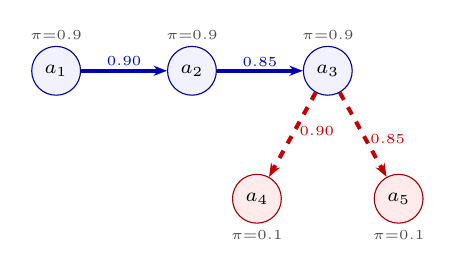
\begin{tikzpicture}[x=15mm, y=13mm]
  % --- the three TRUE claims: a support chain ----------------------------
  \node[atomtrue]  (a1) at (0,0)    {$a_1$};
  \node[atomtrue]  (a2) at (1.15,0) {$a_2$};
  \node[atomtrue]  (a3) at (2.3,0)  {$a_3$};
  % --- the two FALSE claims: attributed and rejected ---------------------
  \node[atomfalse] (a4) at (1.7,-1.25) {$a_4$};
  \node[atomfalse] (a5) at (2.9,-1.25) {$a_5$};

  \node[prlab,above=0.4mm of a1] {$\pi{=}0.9$};
  \node[prlab,above=0.4mm of a2] {$\pi{=}0.9$};
  \node[prlab,above=0.4mm of a3] {$\pi{=}0.9$};
  \node[prlab,below=0.4mm of a4] {$\pi{=}0.1$};
  \node[prlab,below=0.4mm of a5] {$\pi{=}0.1$};

  \draw[ent,relw=0.90] (a1) -- (a2) node[wlab,above]{$0.90$};
  \draw[ent,relw=0.85] (a2) -- (a3) node[wlab,above]{$0.85$};
  % the rejections: a true claim contradicts each false one
  \draw[con,relw=0.90] (a3) -- (a4) node[wlab,right,pos=0.45]{$0.90$};
  \draw[con,relw=0.85] (a3) -- (a5) node[wlab,right,pos=0.55]{$0.85$};
\end{tikzpicture}}
\caption{\textbf{Response A, coherent.} The three true claims form a support chain
  ($a_1\!\to\!a_2\!\to\!a_3$) and each false claim is \emph{attributed and rejected}
  by a \con{} edge from $a_3$. Every claim ends on the correct side of its own prior:
  $\LCS_{\mm}=0.590$, $\LCS_{\cons}=0.963$, $\log Z=-0.95$.}
\label{fig:pair-coherent}
\end{subfigure}
\hfill
\begin{subfigure}[t]{0.49\textwidth}
\centering
\resizebox{\linewidth}{!}{%
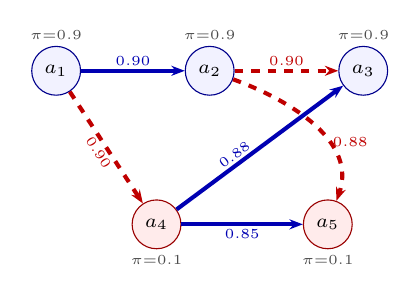
\begin{tikzpicture}[x=15mm, y=13mm]
  \node[atomtrue]  (a1) at (0,0)       {$a_1$};
  \node[atomtrue]  (a2) at (1.3,0)     {$a_2$};
  \node[atomtrue]  (a3) at (2.6,0)     {$a_3$};
  \node[atomfalse] (a4) at (0.85,-1.5) {$a_4$};
  \node[atomfalse] (a5) at (2.3,-1.5)  {$a_5$};

  \node[prlab,above=0.4mm of a1] {$\pi{=}0.9$};
  \node[prlab,above=0.4mm of a2] {$\pi{=}0.9$};
  \node[prlab,above=0.4mm of a3] {$\pi{=}0.9$};
  \node[prlab,below=0.4mm of a4] {$\pi{=}0.1$};
  \node[prlab,below=0.4mm of a5] {$\pi{=}0.1$};

  \draw[ent,relw=0.90] (a1) -- (a2) node[wlab,above]{$0.90$};
  % the response contradicts its own chain ...
  \draw[con,relw=0.90] (a2) -- (a3) node[wlab,above]{$0.90$};
  % ... and leans on a FALSE claim as a load-bearing premise for a TRUE one
  \draw[ent,relw=0.88] (a4) -- (a3) node[wlab,above,sloped,pos=0.38]{$0.88$};
  \draw[con,relw=0.90] (a1) -- (a4) node[wlab,below,sloped]{$0.90$};
  \draw[ent,relw=0.85] (a4) -- (a5) node[wlab,below]{$0.85$};
  \draw[con,relw=0.88] (a2) to[out=-20,in=70] node[wlab,right,pos=0.62]{$0.88$} (a5);
\end{tikzpicture}}
\caption{\textbf{Response B, incoherent.} The same five claims. The response
  contradicts its own chain ($a_2\!\not\to\!a_3$) and makes the false $a_4$ a
  load-bearing premise for the true $a_3$, while $a_1$ and $a_2$ deny $a_4$ and
  $a_5$. The \emph{true} claim $a_3$ is dragged to $0.513$ --- far below its own
  $0.9$ prior: $\LCS_{\mm}=0.494$, $\LCS_{\cons}=0.414$, $\log Z=-3.78$.}
\label{fig:pair-incoherent}
\end{subfigure}
\caption{Relation graphs for the five-claim worked pair (\S\ref{sec-examples}).
  Blue nodes are claims true of the world ($\pi_i=0.9$), red nodes false
  ($\pi_i=0.1$); the \emph{same} five claims appear in both panels. Solid blue:
  \ent{}; dashed red: \con{}. Line width grows with the relation weight $p$.
  The panels differ only in \emph{how the response arranges} the claims, which is
  the whole of what coherence measures --- no per-claim factuality check can
  separate them.}
\label{fig:pair-graphs}
\end{figure}

% The coherence MRF of the five-claim worked pair, drawn as an explicit bipartite
% factor graph: circles are the binary claim variables, squares the factors of
% Eq. eq-joint -- grey unaries phi_i (the priors) and black pairwise psi_r (the
% relations). Styles are in preamble.tex.
\begin{figure}[t]
\centering
\begin{subfigure}[t]{0.49\textwidth}
\centering
\resizebox{\linewidth}{!}{%
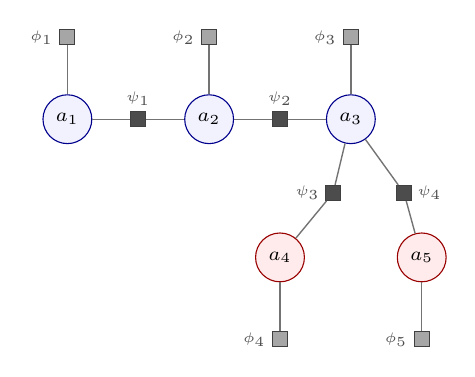
\begin{tikzpicture}[x=15mm, y=13mm]
  \node[atomtrue]  (a1) at (0,0)       {$a_1$};
  \node[atomtrue]  (a2) at (1.2,0)     {$a_2$};
  \node[atomtrue]  (a3) at (2.4,0)     {$a_3$};
  \node[atomfalse] (a4) at (1.8,-1.35) {$a_4$};
  \node[atomfalse] (a5) at (3.0,-1.35) {$a_5$};

  % unary factors phi_i = [1-pi_i, pi_i]
  \node[unary] (p1) at (0,0.8)       {}; \draw[flink] (p1) -- (a1);
  \node[unary] (p2) at (1.2,0.8)     {}; \draw[flink] (p2) -- (a2);
  \node[unary] (p3) at (2.4,0.8)     {}; \draw[flink] (p3) -- (a3);
  \node[unary] (p4) at (1.8,-2.15)   {}; \draw[flink] (p4) -- (a4);
  \node[unary] (p5) at (3.0,-2.15)   {}; \draw[flink] (p5) -- (a5);
  \node[prlab,left=0.4mm of p1] {$\phi_1$};
  \node[prlab,left=0.4mm of p2] {$\phi_2$};
  \node[prlab,left=0.4mm of p3] {$\phi_3$};
  \node[prlab,left=0.4mm of p4] {$\phi_4$};
  \node[prlab,left=0.4mm of p5] {$\phi_5$};

  % pairwise factors psi_r, one per relation
  \node[factor] (f12) at (0.6,0)   {}; \draw[flink] (a1) -- (f12) -- (a2);
  \node[factor] (f23) at (1.8,0)   {}; \draw[flink] (a2) -- (f23) -- (a3);
  \node[factor] (f34) at (2.25,-0.72) {}; \draw[flink] (a3) -- (f34) -- (a4);
  \node[factor] (f35) at (2.85,-0.72) {}; \draw[flink] (a3) -- (f35) -- (a5);
  \node[prlab,above=0.3mm of f12] {$\psi_1$};
  \node[prlab,above=0.3mm of f23] {$\psi_2$};
  \node[prlab,left=0.3mm of f34]  {$\psi_3$};
  \node[prlab,right=0.3mm of f35] {$\psi_4$};
\end{tikzpicture}}
\caption{\textbf{Response A.} Five unaries and four pairwise factors.}
\label{fig:mrf-coherent}
\end{subfigure}
\hfill
\begin{subfigure}[t]{0.49\textwidth}
\centering
\resizebox{\linewidth}{!}{%
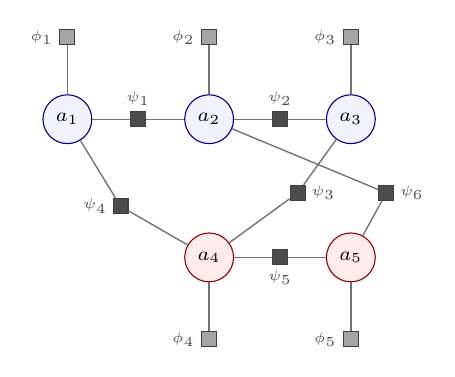
\begin{tikzpicture}[x=15mm, y=13mm]
  \node[atomtrue]  (a1) at (0,0)       {$a_1$};
  \node[atomtrue]  (a2) at (1.2,0)     {$a_2$};
  \node[atomtrue]  (a3) at (2.4,0)     {$a_3$};
  \node[atomfalse] (a4) at (1.2,-1.35) {$a_4$};
  \node[atomfalse] (a5) at (2.4,-1.35) {$a_5$};

  \node[unary] (p1) at (0,0.8)     {}; \draw[flink] (p1) -- (a1);
  \node[unary] (p2) at (1.2,0.8)   {}; \draw[flink] (p2) -- (a2);
  \node[unary] (p3) at (2.4,0.8)   {}; \draw[flink] (p3) -- (a3);
  \node[unary] (p4) at (1.2,-2.15) {}; \draw[flink] (p4) -- (a4);
  \node[unary] (p5) at (2.4,-2.15) {}; \draw[flink] (p5) -- (a5);
  \node[prlab,left=0.4mm of p1] {$\phi_1$};
  \node[prlab,left=0.4mm of p2] {$\phi_2$};
  \node[prlab,left=0.4mm of p3] {$\phi_3$};
  \node[prlab,left=0.4mm of p4] {$\phi_4$};
  \node[prlab,left=0.4mm of p5] {$\phi_5$};

  \node[factor] (f12) at (0.6,0)      {}; \draw[flink] (a1) -- (f12) -- (a2);
  \node[factor] (f23) at (1.8,0)      {}; \draw[flink] (a2) -- (f23) -- (a3);
  \node[factor] (f43) at (1.95,-0.72) {}; \draw[flink] (a4) -- (f43) -- (a3);
  \node[factor] (f14) at (0.45,-0.85) {}; \draw[flink] (a1) -- (f14) -- (a4);
  \node[factor] (f45) at (1.8,-1.35)  {}; \draw[flink] (a4) -- (f45) -- (a5);
  \node[factor] (f25) at (2.7,-0.72)  {}; \draw[flink] (a2) -- (f25) -- (a5);
  \node[prlab,above=0.3mm of f12] {$\psi_1$};
  \node[prlab,above=0.3mm of f23] {$\psi_2$};
  \node[prlab,right=0.3mm of f43] {$\psi_3$};
  \node[prlab,left=0.3mm of f14]  {$\psi_4$};
  \node[prlab,below=0.3mm of f45] {$\psi_5$};
  \node[prlab,right=0.3mm of f25] {$\psi_6$};
\end{tikzpicture}}
\caption{\textbf{Response B.} The same five unaries, but six pairwise factors
  wired so that $\psi_3$ makes a false claim a premise for a true one.}
\label{fig:mrf-incoherent}
\end{subfigure}
\caption{The coherence MRF of Eq.~\ref{eq-joint} for the two responses, as an
  explicit factor graph. Circles are the binary claim variables; grey squares the
  unary factors $\phi_i=[1-\pi_i,\,\pi_i]$ that carry the priors; black squares
  the pairwise factors $\psi_{\tau_r,p_r}$ of Table~\ref{tab:factors}, one per
  mined relation. \textbf{The priors enter only through the $\phi_i$}: the
  claim-level potentials are identical across the two panels, and every difference
  in score comes from the $\psi_r$ --- their number, their endpoints, and their
  couplings.}
\label{fig:pair-mrfs}
\end{figure}


The point of this example is that factuality and coherence are separable, so we hold the first
fixed and vary only the second. Five claims about the Voyager~1 mission are fixed once and for all,
three of them true of the world and two false; stage one is taken as given, contributing the priors
$\pi=0.9$ for each true claim and $\pi=0.1$ for each false one through Eq.~\ref{eq-priors}:

\begin{center}\small
\begin{tabularx}{0.93\textwidth}{@{}l l c X@{}}
\toprule
 & & $\pi_i$ & Claim \\
\midrule
$a_1$ & true  & $0.9$ & Voyager~1 crossed the heliopause in August 2012. \\
$a_2$ & true  & $0.9$ & After the crossing, Voyager~1's instruments measured a sharp rise in plasma density. \\
$a_3$ & true  & $0.9$ & Voyager~1 is therefore in interstellar space. \\
$a_4$ & false & $0.1$ & Voyager~1's plasma wave instrument failed permanently before the crossing. \\
$a_5$ & false & $0.1$ & Voyager~1 has left the Solar System entirely. \\
\bottomrule
\end{tabularx}
\end{center}

Two responses then assert \emph{these same five claims} and differ only in how they arrange them.
Because the claim set is identical, every per-claim factuality check returns the same verdict on
both; the relation graphs (Figure~\ref{fig:pair-graphs}) and the MRFs they induce
(Figure~\ref{fig:pair-mrfs}) are what differ. Table~\ref{tab:pair-responses} gives both responses in
full, with the span asserting each claim marked \claimref{i} at its first mention.

\begin{table}[t]
\centering\small
\begin{tabularx}{0.96\textwidth}{@{}X@{}}
\toprule
\textbf{Response A} (coherent) --- $\LCS_{\mm}=0.590$, $\LCS_{\cons}=0.963$, $\log Z=-0.95$ \\
\midrule
Voyager~1 crossed the heliopause in August 2012,\,\claimref{1} and in the days that followed its
instruments measured a sharp rise in plasma density\,\claimref{2} --- the signature of the denser
medium beyond, and \emph{the measurement that established the boundary had been passed.}
Voyager~1 is therefore in interstellar space.\,\claimref{3} Two persistent misconceptions are
worth clearing up. The first is that the probe's plasma wave instrument had failed permanently
before the crossing;\,\claimref{4} \emph{it cannot have, since it is precisely that instrument
which returned the density profile the conclusion rests on.} The second is that Voyager~1 has
left the Solar System altogether.\,\claimref{5} \emph{Being in interstellar space is not the same
thing: the Sun's gravitational reach extends through the Oort cloud, far beyond the probe's
present distance.} \\
\addlinespace[4pt]
\midrule
\textbf{Response B} (incoherent) --- $\LCS_{\mm}=0.494$, $\LCS_{\cons}=0.414$, $\log Z=-3.78$ \\
\midrule
Voyager~1 crossed the heliopause in August 2012,\,\claimref{1} and after the crossing its
instruments measured a sharp rise in plasma density.\,\claimref{2}
\emph{That said, the probe cannot really be counted as being in interstellar space.}\,\claimref{3} The plasma wave instrument
had in fact failed permanently before the crossing,\,\claimref{4} \emph{and it is precisely that
failure which tells us the probe reached interstellar space.} The instrument failure also means
Voyager~1 has left the Solar System entirely.\,\claimref{5} \emph{Of course, the August 2012
crossing rules out any such permanent failure, and the density measurement is flatly inconsistent
with the probe having left the Solar System.} \\
\bottomrule
\end{tabularx}
\caption{The two responses in full. They assert the \emph{same} five claims of
  \S\ref{sec-example-pair}; each claim's first mention is marked \claimref{i}. Italicized spans are
  the ones the estimator reads as relations. In A they discharge the two false claims; in B they
  reason \emph{from} them.}
\label{tab:pair-responses}
\end{table}

\begin{table}[!ht]
\centering\footnotesize
\setlength{\tabcolsep}{4pt}
\renewcommand{\arraystretch}{1.2}
\caption{The mined relations of both responses, one row per claim pair. \textsc{s} is the Level-2
  discourse sense, $\tau$ the Level-1 coupling it compiles to (Table~\ref{tab:compile}), $p$ the
  weight. \textsc{e} abbreviates \ent{}, \textsc{c} \con{}. These are exactly the edges of
  Figure~\ref{fig:pair-graphs} and the factors $\psi_r$ of Figure~\ref{fig:pair-mrfs}; a dash means
  the response draws no relation over that pair.}
\label{tab:pair-relations}
\begin{tabularx}{\textwidth}{@{}l@{\hspace{7pt}} ll c c@{\hspace{7pt}} ll c c@{\hspace{6pt}} X@{}}
\toprule
& \multicolumn{4}{c@{\hspace{7pt}}}{\textbf{Response A} (coherent)}
& \multicolumn{4}{c@{\hspace{6pt}}}{\textbf{Response B} (incoherent)} & \\
\cmidrule(r{5pt}){2-5}\cmidrule(r{4pt}){6-9}
Pair & Edge & \textsc{s} & $\tau$ & $p$ & Edge & \textsc{s} & $\tau$ & $p$ & What differs \\
\midrule
$\{a_1,a_2\}$ & $a_1\!\to\!a_2$ & \sense{Cau-Eff} & \textsc{e} & $.90$
              & $a_1\!\to\!a_2$ & \sense{Cau-Eff} & \textsc{e} & $.90$
  & The one relation both agree on. \\
$\{a_2,a_3\}$ & $a_2\!\to\!a_3$ & \sense{Evidence} & \textsc{e} & $.85$
              & $a_2\!\to\!a_3$ & \sense{Contrast} & \textsc{c} & $.90$
  & A supports its conclusion; B denies it. Support becomes conflict. \\
$\{a_3,a_4\}$ & $a_3\!\to\!a_4$ & \sense{Contrast} & \textsc{c} & $.90$
              & $a_4\!\to\!a_3$ & \sense{Evidence} & \textsc{e} & $.88$
  & \textbf{The arrow reverses.} A rejects $a_4$; B makes it a premise. \\
$\{a_3,a_5\}$ & $a_3\!\to\!a_5$ & \sense{Contrast} & \textsc{c} & $.85$
              & \multicolumn{4}{c@{\hspace{6pt}}}{---}
  & A refuses $a_5$; B never draws the distinction. \\
$\{a_4,a_5\}$ & \multicolumn{4}{c@{\hspace{7pt}}}{---}
              & $a_4\!\to\!a_5$ & \sense{Cau-Eff} & \textsc{e} & $.85$
  & B alone chains one falsehood into the other. \\
$\{a_1,a_4\}$ & \multicolumn{4}{c@{\hspace{7pt}}}{---}
              & $a_1\!\to\!a_4$ & \sense{Contrast} & \textsc{c} & $.90$
  & B denies $a_4$, which it had just used as a premise --- this strands $a_3$. \\
$\{a_2,a_5\}$ & \multicolumn{4}{c@{\hspace{7pt}}}{---}
              & $a_2\!\to\!a_5$ & \sense{Contrast} & \textsc{c} & $.88$
  & Likewise for $a_5$: asserted, then denied. \\
\midrule
\textbf{Totals} & \multicolumn{4}{c@{\hspace{7pt}}}{2 \textsc{e}, 2 \textsc{c}}
                & \multicolumn{4}{c@{\hspace{6pt}}}{3 \textsc{e}, 3 \textsc{c}}
  & A's conflicts point \emph{outward}, at the false claims; half of B's point \emph{inward}. \\
\bottomrule
\end{tabularx}
\end{table}

The italicized spans are the ones the estimator reads as relations, and they are the whole
difference between the two. Table~\ref{tab:pair-relations} lays the two relation sets side by side,
one row per claim pair, with each relation's discourse sense and the coupling it compiles to. In A
the false claims are named, attributed, and then refused on a stated ground, which compiles to a
\con{} edge from $a_3$. In B the same falsehoods are named and then \emph{used} --- $a_4$ is offered
as the reason $a_3$ holds --- while the response also denies $a_3$ outright and, in its last
sentence, denies $a_4$ and $a_5$ too. Mentioning a falsehood is not what costs B its score;
asserting it and reasoning from it is. All values below are exact, by $2^5=32$-world enumeration.

\begin{example}[Coherent]
\label{ex-pair-coherent}
Response~A's four relations (Table~\ref{tab:pair-relations}, column~A) are a two-edge support chain
over the true claims and one rejection of each false claim. The model returns $\LCS_{\mm}=0.590$ and
$\LCS_{\cons}=0.963$ with $\log Z=-0.95$. Every claim finishes on the correct side of its own prior:
the true claims sit at $0.939$, $0.989$ and $0.992$ --- each \emph{above} its $0.9$ prior, because
the chain supplies mutual support --- and the false ones at $0.013$ and $0.020$, pushed below $0.1$
by the rejections. Nothing in the response fights anything else, so no claim is penalized.
\end{example}

\begin{example}[Incoherent]
\label{ex-pair-incoherent}
Response~B keeps only $a_1\!\to\!a_2$ and replaces the rest with six relations that pull against each
other (Table~\ref{tab:pair-relations}, column~B): it denies its own conclusion, promotes the false
$a_4$ to a premise for that same conclusion, chains $a_4$ into $a_5$, and then denies both
falsehoods in its closing sentence. Three of its six relations are conflicts, and two of those point
at claims the response itself asserts. The score falls to $\LCS_{\mm}=0.494$ and $\LCS_{\cons}=0.414$, with $\log Z=-3.78$. The diagnostic that
localizes the damage is per-claim: the \emph{true} $a_3$ is dragged to $0.513$, far below its own
$0.9$ prior, because its only support arrives from $a_4$, which the response itself denies --- and a
premise the text refuses cannot transmit support. Three claims finish below their own priors,
against two in Response~A, and $a_3$ is the one that matters: a claim true of the world, demoted to
a coin flip by the argument built around it.
\end{example}

Two things are worth reading off this pair. First, the priors enter \emph{only} through the unary
factors $\phi_i$ of Figure~\ref{fig:pair-mrfs}, which are identical in both panels; the entire
$0.590\to0.494$ drop is produced by the $\psi_r$, so it is attributable to arrangement alone.
Second, a claim being true of the world does not protect it: coherence is a property of the joint
distribution, and $a_3$ is suppressed by \emph{how} it is argued for, not by what it says. This is
the mechanism Remark~\ref{rem-order} anticipates and the ordering pair of
\S\ref{sec-example-order} exhibits at scale.

A caution on readouts. $\LCS_{\lp}$ is $0.194$ for Response~A and $0.267$ for Response~B, which
inverts the order --- correctly, and for a reason Eq.~\ref{eq-logz} makes plain: its references
$\log Z_{\max}$ and $\log Z_{\min}$ are recomputed \emph{per response} ($-0.49$ and $-1.06$ for A,
$-1.65$ and $-4.55$ for B), so it reports how close a response comes to the ceiling of \emph{its
own} edge skeleton, not how the two responses compare. It is a within-response diagnostic. Raw
$\log Z$ is comparable across responses and moves the right way, by $2.83$ nats.

\subsection{Response B at two levels of resolution}
\label{sec-example-b-anatomy}

% ---------------------------------------------------------------------------
% Response B, anatomized: the relation graph and the MRF it induces, side by
% side, with the four LCS readouts and the per-claim marginals below them.
%
% The point of putting the two views next to each other is that they are the
% SAME object at two levels of resolution: every edge on the left becomes one
% black pairwise factor on the right, and the five priors that are implicit on
% the left become the five grey unary factors that are explicit on the right.
% The score panel then shows what inference over that MRF returns.
%
% Both panels are drawn at one shared scale (\rbx/\rby) rather than each in its
% own \resizebox, so neither can appear larger than the other. Node, edge and
% relw=p styles live in preamble.tex, shared with figures/graph-coherence-pair,
% mrf-coherence-pair and motivating-example, so no panel can drift.
%
% Every number is produced by scripts/lcs_worked_pair.py from
% data/lcs/example-7-coherence-pair.json -- exact, 2^5 = 32-world enumeration,
% computed twice by independent paths and asserted equal.
% ---------------------------------------------------------------------------
\begin{figure}[tbp]
\centering
\newcommand{\rbx}{13.4mm}
\newcommand{\rby}{11.8mm}

%% ===== (a) the relation graph | (b) the MRF ==============================
\begin{tabularx}{\textwidth}{@{}X@{\hspace{4pt}}X@{}}
\begin{minipage}[b]{\linewidth}\centering
\begin{tikzpicture}[x=\rbx, y=\rby]
  \node[atomtrue]  (a1) at (0,0)        {$a_1$};
  \node[atomtrue]  (a2) at (1.2,0)      {$a_2$};
  \node[atomtrue]  (a3) at (2.4,0)      {$a_3$};
  \node[atomfalse] (a4) at (0.6,-1.6)   {$a_4$};
  \node[atomfalse] (a5) at (1.85,-1.6)  {$a_5$};

  \node[prlab,above=0.4mm of a1] {$\pi{=}.9$};
  \node[prlab,below=0.4mm of a2] {$\pi{=}.9$};
  \node[prlab,above=0.4mm of a3] {$\pi{=}.9$};
  \node[prlab,left=0.5mm of a4]  {$\pi{=}.1$};
  \node[prlab,right=0.5mm of a5] {$\pi{=}.1$};

  \draw[ent,relw=0.90] (a1) -- (a2) node[wlab,above]{$.90$};
  \draw[con,relw=0.90] (a2) -- (a3) node[wlab,above]{$.90$};
  \draw[ent,relw=0.88] (a4) -- (a3)
        node[wlab,above left=-0.4mm and -1.1mm,pos=0.32]{$.88$};
  \draw[con,relw=0.90] (a1) -- (a4) node[wlab,left,pos=0.55]{$.90$};
  \draw[ent,relw=0.85] (a4) -- (a5) node[wlab,below]{$.85$};
  \draw[con,relw=0.88] (a2) to[out=-8,in=25]
        node[wlab,right,pos=0.55,inner sep=1pt]{$.88$} (a5);

  \path (0.6,-2.35) -- (0.6,0.95);   % strut: match the right panel's depth
\end{tikzpicture}\\[2pt]
{\scriptsize \textbf{(a) The relation graph:} three \ent{} (solid blue),\\
 three \con{} (dashed red); width grows with $p$.}
\end{minipage}
&
\begin{minipage}[b]{\linewidth}\centering
\begin{tikzpicture}[x=\rbx, y=\rby]
  \node[atomtrue]  (a1) at (0,0)        {$a_1$};
  \node[atomtrue]  (a2) at (1.15,0)     {$a_2$};
  \node[atomtrue]  (a3) at (2.3,0)      {$a_3$};
  \node[atomfalse] (a4) at (1.15,-1.3)  {$a_4$};
  \node[atomfalse] (a5) at (2.3,-1.3)   {$a_5$};

  % unary factors phi_i = [1-pi_i, pi_i]: the priors, made explicit
  \node[unary] (p1) at (0,0.78)     {}; \draw[flink] (p1) -- (a1);
  \node[unary] (p2) at (1.15,0.78)  {}; \draw[flink] (p2) -- (a2);
  \node[unary] (p3) at (2.3,0.78)   {}; \draw[flink] (p3) -- (a3);
  \node[unary] (p4) at (1.15,-2.08) {}; \draw[flink] (p4) -- (a4);
  \node[unary] (p5) at (2.3,-2.08)  {}; \draw[flink] (p5) -- (a5);
  \node[prlab,left=0.4mm of p1] {$\phi_1$};
  \node[prlab,left=0.4mm of p2] {$\phi_2$};
  \node[prlab,left=0.4mm of p3] {$\phi_3$};
  \node[prlab,left=0.4mm of p4] {$\phi_4$};
  \node[prlab,left=0.4mm of p5] {$\phi_5$};

  % Pairwise factors psi_r, one per mined relation. The two crossing links
  % (a4->a3 and a2->a5) are routed around opposite sides so neither factor
  % sits on the other's edge.
  \node[factor] (f12) at (0.575,0)      {}; \draw[flink] (a1) -- (f12) -- (a2);
  \node[factor] (f23) at (1.725,0)      {}; \draw[flink] (a2) -- (f23) -- (a3);
  \node[factor] (f43) at (1.72,-0.62)   {}; \draw[flink] (a4) -- (f43) -- (a3);
  \node[factor] (f14) at (0.42,-0.80)   {}; \draw[flink] (a1) -- (f14) -- (a4);
  \node[factor] (f45) at (1.725,-1.3)   {}; \draw[flink] (a4) -- (f45) -- (a5);
  \node[factor] (f25) at (2.82,-0.62)   {};
  \draw[flink] (a2) to[out=-32,in=118] (f25);
  \draw[flink] (f25) to[out=-118,in=32] (a5);
  \node[prlab,above=0.3mm of f12] {$\psi_1$};
  \node[prlab,above=0.3mm of f23] {$\psi_2$};
  \node[prlab,left=0.4mm of f43]  {$\psi_3$};
  \node[prlab,left=0.3mm of f14]  {$\psi_4$};
  \node[prlab,below=0.3mm of f45] {$\psi_5$};
  \node[prlab,right=0.4mm of f25] {$\psi_6$};
\end{tikzpicture}\\[2pt]
{\scriptsize \textbf{(b) The MRF it induces:} one $\psi_r$ per edge (black),\\
 one $\phi_i$ per prior (grey).}
\end{minipage}
\end{tabularx}

\medskip
%% ===== (c) the scores ====================================================
% Bands (c) and the per-claim gloss are paper-only: the standalone PNG built by
% scripts/make_response_b_png.sh keeps just the two plots, so \rbnocaption gates
% this block and the \caption below alike.
\ifdefined\rbnocaption\else
\begin{tabularx}{\textwidth}{@{}l@{\hspace{7pt}}c@{\hspace{7pt}}X@{}}
\toprule
Readout & Value & What it says \\
\midrule
$\LCS_{\mm}$ (selected) & $\mathbf{0.494}$
  & Mean posterior marginal: the expected fraction of B's claims its own argument
    upholds. Against a prior-only mean of $0.580$, the arrangement \emph{costs}
    B support rather than adding any. \\
$\LCS_{\cons}$ & $0.414$
  & Two-term consistency: little over a coin flip that no asserted conflict is
    realized, against $0.963$ for the coherent arrangement of the same claims. \\
$\LCS_{\rei}$ & $0.348$
  & The reified-node variant, for comparison; it agrees on the ordering. \\
$\log Z$ & $-3.78$
  & Global mass surviving the constraints ($-0.95$ for the coherent
    arrangement): the six factors are jointly hard to satisfy. \\
\midrule
$\LCS_{\lp}$ & $(0.267)$
  & Parenthesized because it is \emph{not} comparable across responses: its
    references $\log Z_{\max}=-1.65$ and $\log Z_{\min}=-4.55$ are rebuilt from
    B's own edge skeleton, so it reports distance to \emph{that} ceiling. A
    within-response diagnostic only. \\
\bottomrule
\end{tabularx}

\smallskip
{\footnotesize\raggedright
\textbf{Per-claim marginals} (the diagnostic the scalar cannot give):
$a_1\,0.960$, $a_2\,0.973$, $\mathbf{a_3\,0.513}$, $a_4\,0.006$, $a_5\,0.018$.
Three of five finish below their own prior. The one that matters is $a_3$: a claim
\emph{true of the world}, with prior $0.9$, dragged to a coin flip. Its only support
is $\psi_3$, arriving from the false $a_4$ --- which $\psi_4$ has the response
denying. A premise the text refuses cannot transmit support, so $a_3$ is left
holding an argument that undercuts itself. All values exact, by $2^5{=}32$-world
enumeration.\par}

\caption{\textbf{Response B, anatomized.} The incoherent arrangement of the
  five-claim pair (\S\ref{sec-example-pair}) at two levels of resolution, and what
  inference over it returns. Left: the relation graph, blue nodes true of the world
  and red false. Right: the Markov random field of Def.~\ref{def-mrf} that graph
  induces, as an explicit factor graph --- the mapping is one-to-one, six edges to
  six pairwise factors $\psi_r$, five priors to five unary factors $\phi_i$. Below:
  the four readouts of \S\ref{sec-readouts} and the per-claim marginals. The reading to
  take from the pair is that the $\phi_i$ are identical to those of the coherent
  arrangement --- the claim set and every factuality verdict are unchanged --- so the
  whole of the score difference is carried by the $\psi_r$, and the whole of the
  damage is localized by the marginals to $a_3$.}
\label{fig:response-b-anatomy}
\fi
\end{figure}


The pair above varies the arrangement and reads off the difference. It is worth pausing on one of
the two responses on its own, because the step from a relation graph to a probability model is the
step at which most of the modelling content sits, and on a five-claim instance it can be shown in
full rather than described. Figure~\ref{fig:response-b-anatomy} puts Response~B's relation graph
next to the MRF that graph induces, and lists what inference over that MRF returns.

The two panels are the same object at two resolutions, and the translation between them is
mechanical: Def.~\ref{def-mrf} sends each mined relation to exactly one pairwise factor and each
claim to exactly one unary, so B's six edges become $\psi_1,\dots,\psi_6$ and its five priors become
$\phi_1,\dots,\phi_5$. Nothing is added in the crossing and nothing is dropped; what the right panel
supplies is that the priors, implicit in the node colours on the left, become factors of the same
kind as the relations, and therefore quantities the inference trades off against one another. This
is what makes the two-stage composition of \S\ref{sec-twostage} a substitution rather than a
redesign: replacing a uniform $\phi_i$ with a factuality posterior changes a number in an existing
slot.

Three things in the score panel are worth reading off. First, $\LCS_{\mm}=0.494$ sits \emph{below}
the prior-only mean of $0.580$, so B's argument is not merely failing to add support --- it is
removing some, which a measure that only counted satisfied relations could not report
(Prop.~\ref{prop-vacuous}). Second, the readouts agree on the ordering where they are entitled to:
$\LCS_{\mm}$, $\LCS_{\cons}$, $\LCS_{\rei}$ and raw $\log Z$ all place B below the coherent
arrangement, while $\LCS_{\lp}$ is parenthesized because its references are rebuilt per response and
so cannot be compared across the pair. Third, and the reason a scalar is not the whole output, the
per-claim marginals localize the damage: $a_3$ is true of the world and carries a $0.9$ prior, yet
finishes at $0.513$. Reading the mechanism off the right panel, $a_3$'s only support is $\psi_3$,
which arrives from $a_4$; but $\psi_4$ encodes the response denying $a_4$, and $\psi_2$ has it
denying $a_3$ directly. A premise the text refuses cannot transmit support, so the claim that
should have been B's conclusion is left at a coin flip --- by the argument built around it rather
than by anything it says.

\subsection{A sixteen-claim recall report}
\label{sec-example-aero}

% Relation graphs for the AeroParts running example.
% Edges transcribe AEROPARTS_BASE_5 / its conflict-free subset exactly
% (tests/test_lcs_relation_miner.py:83-119). Line width grows with p.
\begin{figure}[t]
\centering
\begin{subfigure}[t]{0.49\textwidth}
\centering
\resizebox{\linewidth}{!}{%
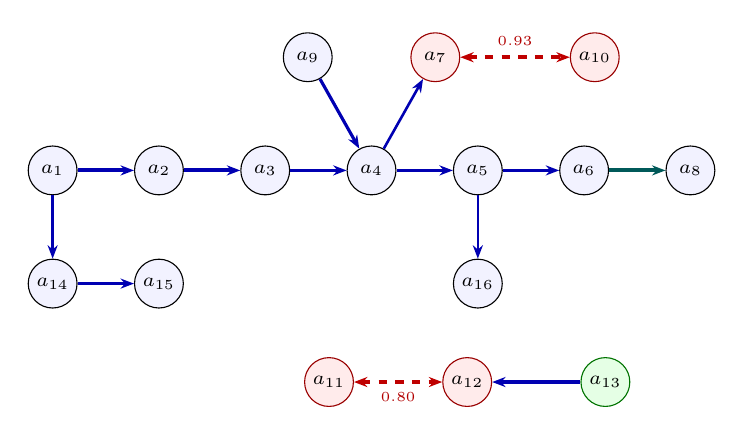
\begin{tikzpicture}[
    >={Stealth[length=1.7mm]},
    atom/.style={circle,draw,fill=blue!5,inner sep=0.5pt,minimum size=6.2mm,font=\scriptsize},
    conf/.style={circle,draw,fill=red!8,draw=red!60!black,inner sep=0.5pt,
                 minimum size=6.2mm,font=\scriptsize},
    hold/.style={circle,draw,fill=green!10,draw=green!45!black,inner sep=0.5pt,
                 minimum size=6.2mm,font=\scriptsize},
    ent/.style={-{Stealth[length=1.7mm]},blue!70!black},
    equ/.style={-{Stealth[length=1.7mm]},teal!70!black},
    xcl/.style={{Stealth[length=1.7mm]}-{Stealth[length=1.7mm]},red!75!black,dashed},
    x=13.5mm, y=12.5mm]

  % ---- the entailment spine, left to right ----
  \node[atom] (a1) at (0,0)   {$a_1$};
  \node[atom] (a2) at (1,0)   {$a_2$};
  \node[atom] (a3) at (2,0)   {$a_3$};
  \node[atom] (a4) at (3,0)   {$a_4$};
  \node[atom] (a5) at (4,0)   {$a_5$};
  \node[atom] (a6) at (5,0)   {$a_6$};
  \node[atom] (a8) at (6,0)   {$a_8$};
  % ---- branches ----
  \node[atom] (a9)  at (2.4,1.15) {$a_9$};
  \node[conf] (a7)  at (3.6,1.15) {$a_7$};
  \node[atom] (a14) at (0,-1.15)  {$a_{14}$};
  \node[atom] (a15) at (1,-1.15)  {$a_{15}$};
  \node[atom] (a16) at (4,-1.15)  {$a_{16}$};
  % ---- the blame sub-argument ----
  \node[conf] (a10) at (5.1,1.15)  {$a_{10}$};
  \node[conf] (a11) at (2.6,-2.15) {$a_{11}$};
  \node[conf] (a12) at (3.9,-2.15) {$a_{12}$};
  \node[hold] (a13) at (5.2,-2.15) {$a_{13}$};

  \draw[ent,line width=1.50pt] (a1) -- (a2);
  \draw[ent,line width=1.42pt] (a2) -- (a3);
  \draw[ent,line width=1.10pt] (a3) -- (a4);
  \draw[ent,line width=1.30pt] (a4) -- (a5);
  \draw[ent,line width=1.22pt] (a5) -- (a6);
  \draw[ent,line width=0.94pt] (a4) -- (a7);
  \draw[ent,line width=1.14pt] (a9) -- (a4);
  \draw[equ,line width=1.46pt] (a6) -- (a8);
  \draw[ent,line width=1.26pt] (a1) -- (a14);
  \draw[ent,line width=1.10pt] (a14) -- (a15);
  \draw[ent,line width=0.86pt] (a5) -- (a16);
  \draw[ent,line width=1.42pt] (a13) -- (a12);

  % ---- the two conflicts: what makes this response incoherent ----
  \draw[xcl,line width=1.58pt] (a7) -- (a10)
        node[midway,above,font=\tiny,red!70!black]{$0.93$};
  \draw[xcl,line width=1.30pt] (a11) -- (a12)
        node[midway,below,font=\tiny,red!70!black]{$0.80$};
\end{tikzpicture}}
\caption{\textbf{Incoherent} (base). Two \coupling{exclusive} conflicts (dashed):
  $a_7\!\leftrightarrow\!a_{10}$ is \emph{unresolved}; $a_{11}\!\leftrightarrow\!a_{12}$
  is a concession the holding $a_{13}$ (green) resolves.
  $\readout{mm}=0.607$, $\log Z=-9.64$.}
\label{fig:aero-incoherent}
\end{subfigure}
\hfill
\begin{subfigure}[t]{0.49\textwidth}
\centering
\resizebox{\linewidth}{!}{%
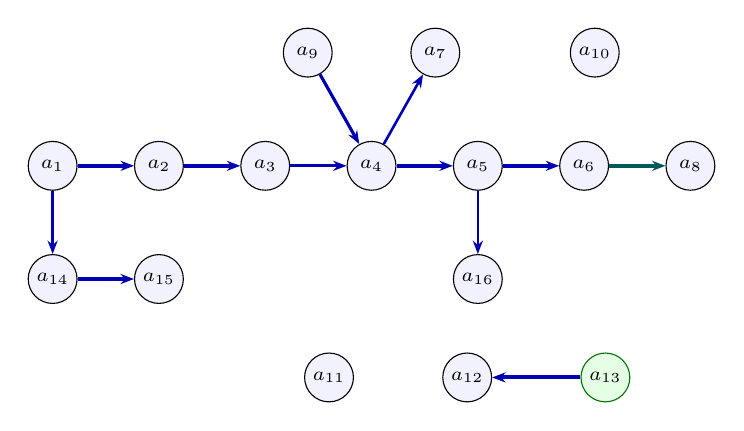
\begin{tikzpicture}[
    >={Stealth[length=1.7mm]},
    atom/.style={circle,draw,fill=blue!5,inner sep=0.5pt,minimum size=6.2mm,font=\scriptsize},
    hold/.style={circle,draw,fill=green!10,draw=green!45!black,inner sep=0.5pt,
                 minimum size=6.2mm,font=\scriptsize},
    ent/.style={-{Stealth[length=1.7mm]},blue!70!black},
    equ/.style={-{Stealth[length=1.7mm]},teal!70!black},
    x=13.5mm, y=12.5mm]

  \node[atom] (a1) at (0,0)   {$a_1$};
  \node[atom] (a2) at (1,0)   {$a_2$};
  \node[atom] (a3) at (2,0)   {$a_3$};
  \node[atom] (a4) at (3,0)   {$a_4$};
  \node[atom] (a5) at (4,0)   {$a_5$};
  \node[atom] (a6) at (5,0)   {$a_6$};
  \node[atom] (a8) at (6,0)   {$a_8$};
  \node[atom] (a9)  at (2.4,1.15) {$a_9$};
  \node[atom] (a7)  at (3.6,1.15) {$a_7$};
  \node[atom] (a14) at (0,-1.15)  {$a_{14}$};
  \node[atom] (a15) at (1,-1.15)  {$a_{15}$};
  \node[atom] (a16) at (4,-1.15)  {$a_{16}$};
  \node[atom] (a10) at (5.1,1.15)  {$a_{10}$};
  \node[atom] (a11) at (2.6,-2.15) {$a_{11}$};
  \node[atom] (a12) at (3.9,-2.15) {$a_{12}$};
  \node[hold] (a13) at (5.2,-2.15) {$a_{13}$};

  \draw[ent,line width=1.50pt] (a1) -- (a2);
  \draw[ent,line width=1.42pt] (a2) -- (a3);
  \draw[ent,line width=1.10pt] (a3) -- (a4);
  \draw[ent,line width=1.30pt] (a4) -- (a5);
  \draw[ent,line width=1.22pt] (a5) -- (a6);
  \draw[ent,line width=0.94pt] (a4) -- (a7);
  \draw[ent,line width=1.14pt] (a9) -- (a4);
  \draw[equ,line width=1.46pt] (a6) -- (a8);
  \draw[ent,line width=1.26pt] (a1) -- (a14);
  \draw[ent,line width=1.10pt] (a14) -- (a15);
  \draw[ent,line width=0.86pt] (a5) -- (a16);
  \draw[ent,line width=1.42pt] (a13) -- (a12);
\end{tikzpicture}}
\caption{\textbf{Coherent}. The identical support structure with both conflict edges
  removed; $a_{10}$ and $a_7$ are no longer suppressed.
  $\readout{mm}=0.620$, $\log Z=-8.25$, $\readout{lp}=1.00$.}
\label{fig:aero-coherent}
\end{subfigure}
\caption{Relation graphs for the AeroParts recall report
  (\S\ref{sec-examples}). Solid blue: \coupling{entailment}; teal:
  \coupling{equivalence}; dashed red, double-headed: \coupling{exclusive}. Line
  width grows with the relation weight $p$. \textbf{The two panels differ only in
  the two conflict edges}, so the $0.607\!\to\!0.620$ lift and the $1.39$ nats of
  recovered mass are attributable to conflict structure alone.}
\label{fig:aero-graphs}
\end{figure}


The second example is a sixteen-claim aviation recall report, which exercises the conflict taxonomy
more fully than the five-claim pair: it carries both an unresolved conflict and a conceded one. Its
relation graph is twelve support edges ---
an entailment spine $a_1\!\to\!a_2\!\to\!\dots\!\to\!a_6$ (shipment certified to spec, installation,
entry into service, in-flight failures, regulatory probe, grounding order), branches to the
pulled-from-service claim, the maintenance-log evidence, the tribunal's damages award and the
regulator's bulletin, and one \eqv{} edge --- plus two conflicts. Every value below is exact, by
$2^{16}$ enumeration, and the graph is reproduced edge-by-edge in Figure~\ref{fig:aero-graphs} with
each edge's weight shown by line thickness.

\begin{example}[Incoherent]
\label{ex-incoherent}
The report asserts both that \emph{no passengers or crew were harmed} and that a wire report
\emph{claimed three passengers died}. These are exhaustive alternatives rather than mere opposition:
they cannot both hold and cannot both fail, so the relation is \exc{} with $p=0.93$ --- and nothing in
the response resolves it. A second tension, between the airline's pilot-error argument and the final
report's metallurgical-defect finding ($p=0.80$), is a \sense{Concession} that the tribunal's holding
does resolve, and Eq.~\ref{eq-concession} discounts it accordingly. The model returns
$\LCS_{\mm}=0.607$ with $\log Z=-9.64$. The diagnostic that localizes the incoherence is per-claim: the
marginal of the claim on the losing side of the \emph{unresolved} conflict is dragged \emph{below its
own prior}, which no aggregate score would reveal. Applying the concession discount alone --- resolving
the second tension while leaving the first --- raises the score to $0.612$, as C2 requires.
\end{example}

\begin{example}[Coherent]
\label{ex-coherent}
Removing the two conflict edges and changing nothing else leaves the identical support structure
(Figure~\ref{fig:aero-coherent}). The score rises to $\LCS_{\mm}=0.620$ with $\log Z=-8.25$ and
$\LCS_{\lp}=1.00$: the response is now as coherent as its own edge skeleton permits, which is what the
ceiling of Eq.~\ref{eq-logz} means. The suppressed claim recovers to its prior.
\end{example}

Because the two panels of Figure~\ref{fig:aero-graphs} differ \emph{only} in the two conflict edges,
the $0.607\to0.620$ lift and the $1.39$ nats of recovered probability mass are attributable to conflict
structure alone --- which is the property the ladder construction of \S\ref{sec-locobench} generalizes
from one pair to a family. The full ladder over this family is monotone throughout:
$0.586 < 0.607 < 0.612 < 0.613 < 0.620$ over the rungs \emph{worse}, \emph{base},
\emph{concession-resolved}, \emph{one-conflict-fixed}, \emph{coherent}.\footnote{Treating both tensions
as plain \con{} rather than \exc{} --- the three-coupling model that omits the exhaustiveness
distinction --- gives $\LCS_{\mm}=0.587$ and $\log Z=-9.75$ for Example~\ref{ex-incoherent}, with
Example~\ref{ex-coherent} unchanged at $0.620$ and $-8.25$. The distinction of \S\ref{sec-couplings} is
worth $0.020$ of score here, and the reason it matters more than that figure suggests is
Table~\ref{tab:allcands}: with \exc{} conflicts, readout (b)'s conflict term is pinned at $1.000$ and
the readout fails outright.}

\subsection{A claim-identical ordering pair}
\label{sec-example-order}

This pair makes the order-sensitivity claim concretely. Two summaries of one appellate
judgment are built from an \emph{identical} set of eighteen claims --- the same atom texts, one a
permutation of the other --- differing only in whether self-serving assertions precede or follow the
findings that qualify them. The faithful ordering scores $\LCS_{\mm}=0.95$ and the
self-serving-first ordering $0.90$. No per-claim factuality check can separate them, because every
claim is byte-identical; what differs is which claims the response leaves standing unqualified at the
point where it asserts them.

It is worth being exact about \emph{how} the two scores differ, because Remark~\ref{rem-order} might
seem to forbid it: nothing in Eq.~\ref{eq-joint} references position, so an edit preserving the
relation set cannot move any readout. The pair does not preserve the relation set. Mining is
response-grounded (\S\ref{sec-mining}), so the relations the estimator draws are a function of the
prose, not of the claim list: the faithful summary states each tension beside the truth or holding
that settles it, which the estimator reads as a \sense{Concession} the text resolves and
Eq.~\ref{eq-concession} discounts; the adversarial summary leaves the same claims standing
unqualified until a later holding overrides them, which reads as a live conflict. The claim set is
what factuality sees and it is identical; the relation set is what coherence sees and it is not.

%% ================================================================
\section{Limitations}
\label{sec-limitations}
%% ================================================================

\paragraph{The model is pairwise, and some incoherence is not.} Definition~\ref{def-mrf} admits only
pairwise factors, so genuinely $k$-ary structure lies outside the family. This is the sharpest
limitation of the measure and it is worth stating exactly rather than in passing, because it is not a
matter of degree: the relevant conflicts are not approximated badly, they are unrepresentable.

\begin{proposition}[Jointly inconsistent, pairwise consistent]
\label{prop-kary}
Let $\pr{\mathbf{a}}$ factorize as in Eq.~\ref{eq-joint} over $a_1,a_2,a_3$ with non-negative
factors. If $\pr{a_1{=}1,a_2{=}1,a_3{=}1}=0$ then $\pr{a_i{=}1,a_j{=}1}=0$ for some pair $i\neq j$.
Consequently no member of the family represents ``the three claims cannot all hold, but any two
can''.
\end{proposition}

\begin{proof}
By Eq.~\ref{eq-joint}, $\pr{1,1,1}=Z^{-1}\prod_i\phi_i(1)\prod_{i<j}\psi_{ij}(1,1)$, a product of
non-negative terms, which vanishes only if some term does. If $\phi_i(1)=0$ then $a_i$ is false
almost surely and both pairs containing $i$ have probability zero. If $\psi_{ij}(1,1)=0$ then every
world with $a_i=a_j=1$ carries that factor, so $\pr{a_i{=}1,a_j{=}1}=0$ directly. A ternary factor
that vanishes only at $(1,1,1)$ has neither consequence.
\end{proof}

The gap is quantitative as well as qualitative. With uniform priors, a ternary factor supported off
$(1,1,1)$ gives $\pr{1,1,1}=0$ while leaving each pair jointly true with probability $0.143$; the
best pairwise attempt that drives $\pr{1,1,1}$ below $10^{-4}$ leaves the pairs at $0.028$, and a
random search over $2\times10^{5}$ pairwise parameterizations found nothing better. The pairwise model
can only suppress the bad world by also suppressing the good ones that share a $(1,1)$ cell with it.
Every figure in this paragraph is exact by $2^3$ enumeration and reproduced by a released script and
regression test, so the proposition is checked and not merely asserted.

This is not a hypothetical. Prompting a frontier model to plant a single arithmetic inconsistency in
an otherwise ordinary encyclopedic paragraph produced a passage whose decomposition places the
conflict across \emph{three} claims: that a league comprises $356$ teams, that those teams form $32$
conferences, and that each conference has exactly $10$ member schools. No two of the three conflict;
$32\times10\neq356$ requires all three. Mining that passage with the estimator of
\S\ref{sec-mining} returns \emph{zero} conflict edges, and the readouts accordingly report it as
coherent ($\LCS_{\mm}=0.68$, $\LCS_{\lp}=1.00$). The omission is not an extraction failure: run under
the \texttt{all\_pairs} policy, which scores every one of the $\binom{n}{2}$ candidate pairs, the
result is unchanged, and querying the estimator on each of the three pairs in isolation returns
\coupling{none} or \ent{} --- never a conflict. Proposition~\ref{prop-kary} says no reweighting of
those factors could have helped.

Two milder consequences of the same restriction are worth naming. Transitivity is not enforced ---
the model will happily hold $a\Rightarrow b$ and $b\Rightarrow c$ at high weight while leaving $a$ and
$c$ unrelated, since it has no rule tying them. And a claim conceded by two independent holdings is
discounted twice rather than once. All three are expressible as first-order rules in the Markov logic
view of Appendix~\ref{app-mln}, which is the natural route past this limitation and which we have not
taken; Remark~\ref{rem-closed}'s closure guarantee is precisely what buys tractability here and
precisely what costs us this class of defect.

\paragraph{Hand-set constants.} The design deliberately avoids free parameters --- criterion R4 exists
for that reason, and it is what disqualifies readout (c) with its prior $\rho$. Two constants remain.
The concession discount $\lambda=0.45$ in Eq.~\ref{eq-concession} sets how much a resolved tension is
softened, and the resolver-detection heuristic identifies holdings by cue phrases and lexical overlap.
Both are defensible and neither is derived. A principled treatment would learn the discount from
labelled resolved and unresolved concessions, which the corpus of \S\ref{sec-locobench} supplies in
principle but not at the scale required.

\paragraph{Relation estimation dominates the error.} \S\ref{sec-experiments} is unambiguous that the
bottleneck is not the model. At $56.3\%$ coupling-level F1, roughly half the factors in a mined network
are wrong or missing, and the $25$--$43$ point ladder-agreement gap between mined and gold arms follows
from that. Everything the paper establishes about the readouts is established on gold or exact graphs;
the mined-arm numbers should be read as a measurement of current extraction quality, not as the
measure's ceiling.

\paragraph{Approximate inference is not characterized.} Production inference is weighted mini-bucket
with i-bound $6$, while every exact value reported here comes from $2^n$ enumeration, feasible only for
$n\le20$ claims. The two agree on the fixtures we can check both ways, but we have not characterized
the approximation error at length, and the augmented networks of \S\ref{sec-consistency} --- which add
one auxiliary variable per relation --- are the case where it would most plausibly bite.

\paragraph{Empirical scope.} The generated corpus is fourteen families and seventy items spanning all
four ladder types, with single-sample mining whose measured run-to-run movement is at most $0.014$ F1
across two independent runs of the same configuration. All five baseline families of
\S\ref{sec-baselines} are measured on the ladder corpus (\S\ref{sec-baselines-measured}). On the $50$ readout-independent ladder assertions all three graded
readouts now sit above every evidence-free baseline, which supersedes the tie we reported on ten
assertions; we flag the direction of that correction in \S\ref{sec-baselines-measured} rather than
quietly restating it. \citet{liustrube} is cited rather than run, for the output-type reason given
above.

Three things remain genuinely open. First, the control and order ladders --- the invariance
experiments --- reveal that \emph{mined} graphs are strongly order-dependent ($0/45$ and $0/15$ on
every mined arm, with a five-rung edge count of $9,16,20,20,17$ under pure sentence reordering), and we
cannot yet say how a human annotator would score those same rungs, which is the comparison that would
separate ``the extractor is unstable'' from ``the invariance requirement is too strict''. Second,
human correlation generally, which is what would establish that the construct being ordered is the one
readers care about. Third, judge dependence: the two LLM judges we ran disagree by up to $42$ points
on the identical assertions, so any single-judge number here --- including ours --- carries that
uncertainty. And the corpus is LLM-generated throughout, gold relation labels included, with
LLM-committee validation; a bias shared between generator and committee would not be caught by it.

%% ================================================================
\section{Conclusion}
%% ================================================================

Coherence is a property of a joint distribution over what a response asserts, and it can be read off a
Markov random field whose factors are the relations the response itself draws. Three things follow from
taking that view seriously. First, the factor tables matter: the ones that are right for grounding a
claim against evidence charge a premise for being a premise, and a coherence measure built on them
spends its dynamic range in the wrong place (Prop.~\ref{prop-rowstoch}). Second, the relation
vocabulary can be rich at the annotation layer and must be narrow at the inferential one; twelve
discourse senses compiling deterministically onto five couplings, each fixed by the world it penalizes,
keeps the model a closed pairwise family while leaving the labels interpretable. Third, and least
expected, not every reading of ``how coherent is this?'' is admissible. Of four candidates, two are
non-monotone in conflict resolution for a single diagnosable reason --- they measure whether a conflict
is active rather than what should be believed (Prop.~\ref{prop-quirk}) --- and a fifth, apparently the
most natural of all, is maximized by asserting no relations whatever (Prop.~\ref{prop-vacuous}). The
mean posterior marginal survives all five criteria, needs one inference query, and localizes an
incoherence to the claims responsible.

Measuring such a score requires controlled contrasts, and ladders of responses over one claim set with
declared orderings supply them. Given gold relation graphs the readouts recover $82.7\%$ of those
orderings; given graphs mined from the response text, $34.7$--$37.1\%$. Because the two conditions
differ in nothing but the relation graph, the gap localizes the open problem: the probabilistic model is
adequate, and grounded relation extraction, at $52\%$ coupling-level F1 at best and not invariant to
sentence order, is the bottleneck. That is a
more tractable target than ``measure coherence'', and it is one that improvements can be measured
against.

%%%%%%%%%%%%%%%%%%%%%%%%%%%%%%%%%%%%%%%%%%%%%%%%%%%%%%%%%%%%%%%%%%%%%%%%%%%%%
\subsection*{AI use statement}

Generative AI is both an object of study and a component of the artifacts released here, and we
disclose both roles. The relation estimator of \S\ref{sec-mining} is LLM-based by design: its prompts,
its logprob-derived confidences and its failure modes are contributions of the paper. The evaluation
corpus of \S\ref{sec-locobench} is LLM-generated throughout, including its gold relation labels, and
validated by an independent LLM committee; \S\ref{sec-limitations} states the consequences for treating
it as ground truth. We additionally used AI assistants for code implementation and for editorial
assistance on this manuscript. All LLM-generated code was reviewed by the authors and is covered by a
test suite that pins the exact numerical values reported in \S\ref{sec-examples} and
Table~\ref{tab:allcands}; every number in \S\ref{sec-experiments} was traced to a stored experiment
record. The research questions, the taxonomy, the readout definitions, the propositions and their
proofs are the authors' own. We take responsibility for the final content of this work.

\subsection*{Ethics statement}

This work involves no human subjects and no personally identifying data. The fixtures include a summary
of a published appellate judgment, used as a worked example of ordering-dependent coherence; it is a
matter of public record and no private individual is the subject of analysis. The principal ethical risk
is misreading: a coherence score is not a truth score, and a response can be perfectly coherent and
entirely false. That is precisely why \S\ref{sec-twostage} keeps the two axes separable, and we caution
against deploying $\LCS$ alone as a factuality filter --- a fluent, internally consistent fabrication is
exactly the artifact it scores highest. The released fixtures and corpus deliberately contain false
claims, labelled as such, and should not be redistributed without those labels.

\subsection*{Reproducibility statement}

The model is fully specified in the paper: Definition~\ref{def-mrf} gives the joint,
Table~\ref{tab:factors} both families of potentials, Def.~\ref{def-couplings} the penalized sets,
Table~\ref{tab:compile} the compile map, and Eqs.~\ref{eq-mm}--\ref{eq-logz} the four readouts together
with the auxiliary-variable constructions two of them require. Algorithms~\ref{alg-pairs} and
\ref{alg-lcs} give candidate selection and the end-to-end procedure. Appendix~\ref{app-prompts}
reproduces all four estimation prompts verbatim, including the trailing token boundary that the
surrogate readout depends on. The exact values in \S\ref{sec-examples} and Table~\ref{tab:allcands} are
computed by explicit $2^n$ enumeration --- $2^5$ for the five-claim pair, $2^{16}$ for the recall
report --- and are pinned by regression tests in the released code, so they are reproducible without
LLM access. The relation graphs they use are given edge-by-edge in
Figures~\ref{fig:pair-graphs} and~\ref{fig:aero-graphs}, the five-claim pair's claim set, priors
and gold relations ship as a fixture, and a single script recomputes every number it reports. The
$k$-ary representability figures of \S\ref{sec-limitations} (Prop.~\ref{prop-kary}) are likewise
exact by $2^3$ enumeration, with the seeded random search and the published table both reproduced by
a released script and pinned by regression tests. \S\ref{sec-experiments} names every model used and states the sampling
regime and its measured variance. Code, fixtures and corpus are released.

\bibliography{ref}
\bibliographystyle{iclr2027_conference}

\appendix

%% ================================================================
\section{The estimation prompts, verbatim}
\label{app-prompts}
%% ================================================================

The four prompts below are reproduced exactly as they are issued, extracted programmatically from the
released source so that this appendix cannot drift from the code. Placeholders in double braces are
substituted at call time; \verb|{{sense_menu}}| is substituted at build time from one of the two menus
in \S\ref{app-menus}.

\subsection{Prompt A, first generation --- discourse sense and coupling}
\label{app-prompt-a1}
$6{,}148$ characters. Placeholders: \verb|{{sense_menu}}|, \verb|{{response}}|, \verb|{{atom_a}}|,
\verb|{{atom_b}}|.
\promptfile{prompts/PROMPT_A_V1.txt}

\subsection{Prompt A, second generation --- rebalanced for precision}
\label{app-prompt-a2}
$6{,}361$ characters. Same placeholders. The five changes relative to the first generation, and their
motivation, are given in \S\ref{sec-mining}: few-shot balance from $3{:}1$ related to $2{:}3$; negative
exemplars showing silence rather than explicit disavowal; a verifiable evidence span; the
discriminating question asked first; and \coupling{none} given first position and equal prose.
Transitivity is named as a non-relation.
\promptfile{prompts/PROMPT_A_V2.txt}

\subsection{Prompt B, default --- surrogate-token conditional strength}
\label{app-prompt-b1}
$2{,}182$ characters. Placeholders: \verb|{{response}}|, \verb|{{atom_a}}|, \verb|{{atom_b}}|,
\verb|{{coupling}}| (twice). This is the one prompt that does not end in a newline: it terminates with
\verb|Answer: | including the trailing space, so that the model's next token is the surrogate whose
logprobs are read. Reproducing it without that trailing space changes the tokenization of the answer
position and therefore the estimate.
\promptfile{prompts/PROMPT_B_SURROGATE.txt}

\subsection{Prompt B, baseline --- verbalized conditional strength}
\label{app-prompt-b2}
$2{,}112$ characters. Retained only for the comparison reported in \S\ref{sec-experiments}; verbalized
confidence is weakly calibrated \citep{xiong}.
\promptfile{prompts/PROMPT_B_VERBALIZED.txt}

\subsection{The two sense menus}
\label{app-menus}
The full menu offers all twelve senses of Table~\ref{tab:compile} plus \coupling{none}:
\promptfile{prompts/SENSE_MENU_FULL.txt}
The restricted menu offers only the senses the evaluation corpus labels, which is the admissibility
filter of \S\ref{sec-mining} applied at elicitation time rather than after it:
\promptfile{prompts/SENSE_MENU_GOLD9.txt}
Note that the restricted menu omits \sense{Succession} as well as \sense{Condition} and
\sense{Instantiation}, leaving nine relation-bearing senses. \sense{Succession} is dropped because it is
the mirror of \sense{Precedence} and both compile to \coupling{none}, so offering both invites an
arbitrary choice on a relation that produces no factor either way. The second-generation Prompt A's body
is written against this restricted menu; when it is run with the full menu, three senses are offered
with no gloss and no coupling mapping in the prompt body, and we report which menu each arm used.

%% ================================================================
\section{The reified coherence node, worked}
\label{app-reified}
%% ================================================================

To make Eq.~\ref{eq-reified} concrete, take the three-claim subnet consisting of the unresolved
casualty conflict of Example~\ref{ex-incoherent} together with one entailment feeding it: claims
$a_7,a_{10}$ joined by a conflict at $p=0.93$, and $a_4\to a_7$ an entailment at $p=0.65$, all priors
$\tfrac12$, with $\rho=\tfrac12$. Writing out the eight-cell vote factor for each relation from
Eq.~\ref{eq-reified} and enumerating the $2^4$ worlds of $(a_4,a_7,a_{10},R)$ gives
$\pr{R{=}1}=0.453$: below its prior, because both relations have violating worlds that carry
appreciable mass, and the conflict's violating world $(1,1)$ carries the most.

Two properties of the construction are worth noting. The $R=0$ branch is flat, so $R=0$ asserts nothing
and the node cannot be driven up merely by adding relations that happen to be satisfied. And the factor
is a \emph{noisy} AND rather than a hard one: a relation with $p_r<1$ leaves some mass on its violating
worlds even when $R=1$, so a single strongly-violated relation reduces $\pr{R{=}1}$ without pinning it
to zero. The reason we do not adopt the readout despite this reasonable behaviour is
Table~\ref{tab:allcands}: it dips at the concession variant for the reason of
Prop.~\ref{prop-quirk}, and it requires the free parameter $\rho$, violating R4.

%% ================================================================
\section{Correspondence with Markov logic}
\label{app-mln}
%% ================================================================

The coherence MRF has a natural first-order encoding \citep{mln}, with
$\pr{\mathbf{a}}=\tfrac1Z\exp\bigl(\sum_k w_k n_k(\mathbf{a})\bigr)$ for $n_k(\mathbf{a})$ the number of
true groundings of formula $F_k$. Evidence predicates $\mathit{Entail}(i,j)$,
$\mathit{Contradict}(i,j)$, $\mathit{Equiv}(i,j)$ and $\mathit{Resolves}(h,i,j)$ carry the mined graph;
$\mathit{Holds}(i)$ is the query predicate. Working out the correspondence is instructive in both
directions.

\subsection{The naive encoding is a different model}

The obvious encoding gives each relation one weighted clause, e.g.\
$\mathit{Entail}(i,j)\wedge a_i \Rightarrow a_j$ with $w=\mathrm{logit}(p)$. This is \emph{not}
equivalent to Definition~\ref{def-mrf}. Its induced pairwise factor is $[e^w,e^w,1,e^w]$, which is not
row-stochastic in the sense of Prop.~\ref{prop-rowstoch}: it rewards the vacuous $a_s=0$ rows with
$e^w$ on \emph{both} target states, so a clause is best satisfied by making its antecedent false.
Brute force over the $2^{16}$ worlds of the recall report of \S\ref{sec-example-aero} gives mean
marginal support $0.455$ under
the naive MLN against $0.587$ under the corresponding MRF, with per-claim marginals differing by up to
$0.31$. These are two different models, not two encodings of one.

The failure is sharpest at the mode. The all-false world satisfies every implication vacuously, so under
the naive encoding the most probable configuration of any purely-implicational graph is the one in which
the response asserts nothing --- the maximum-a-posteriori reading of a response is that none of it
holds. This is Prop.~\ref{prop-vacuous} appearing in a second guise, and it is the same lesson: an
encoding that scores rule satisfaction rather than belief can be maximized by having nothing to satisfy.

\subsection{A three-clause expansion is exactly equivalent}

Writing the log-potential in the general pairwise form
$\ln\psi(a_s,a_t)=\alpha+\beta a_s+\gamma a_t+\delta\,a_s a_t$ and matching it against the
with-priors tables of Table~\ref{tab:factors} gives, for $\pi_s$ the source prior and
$\mathrm{L}(x)=\mathrm{logit}(x)$:
\begin{center}\small
\begin{tabular}{@{}lllll@{}}
\toprule
$\tau$ & $\alpha$ (unit) & $\beta$ (source) & $\gamma$ (target) & $\delta$ (conjunction) \\
\midrule
\ent & $\ln(1-\pi_s)$ & $\ln\frac{1-p}{1-\pi_s}$ & $\mathrm{L}(\pi_s)$
     & $+\mathrm{L}(p)-\mathrm{L}(\pi_s)$ \\
\con & $\ln(1-\pi_s)$ & $\ln\frac{p}{1-\pi_s}$   & $\mathrm{L}(\pi_s)$
     & $-\mathrm{L}(p)-\mathrm{L}(\pi_s)$ \\
\eqv & $\ln p$ & $\ln\frac{1-p}{p}$ & $\ln\frac{1-p}{p}$ & $+2\,\mathrm{L}(p)$ \\
\bottomrule
\end{tabular}
\end{center}
At the atom prior $\pi_s=\tfrac12$ the $\mathrm{L}(\pi_s)$ terms vanish, and the table reduces to
$\gamma=0$ with $\delta=\pm\mathrm{L}(p)$: in that setting the conjunction weight \emph{is} exactly
$\pm\mathrm{logit}(p)$, the interaction the implication was meant to carry all along, and the unit and
source clauses are the correction that makes each row a conditional. Away from $\tfrac12$ the
$\mathrm{L}(\pi_s)$ terms are load-bearing, which matters for the two-stage composition of
\S\ref{sec-twostage}, where the priors are factuality posteriors rather than uniform. With this
expansion the ground Markov logic network reproduces the MRF exactly: at $\pi_s=\tfrac12$, mean
support $0.5866$ and $\log Z=-9.751$ for both, with zero per-claim difference to machine precision;
the agreement is verified against the brute-force oracle at priors on and off $\tfrac12$.

We establish the equivalence for the three original couplings only. \exc{} and \cnc{} are not tabulated
here, so the claim ``the MLN encoding reproduces the MRF'' should be read as scoped to the
three-coupling fragment. That is a real limitation for the recall report of
\S\ref{sec-example-aero}, whose conflicts are \exc{}; the five-claim pair of
\S\ref{sec-example-pair} uses \con{} throughout and so falls inside the tabulated fragment.

\subsection{Which view to keep, and why both}

The reason to prefer the MRF for the measure itself is Remark~\ref{rem-closed}: its pairwise factor
family is closed at three parameters, so the inferential vocabulary cannot quietly grow as senses are
added, and every relation type is guaranteed to be a $2\times2$ potential. The reason to keep the
Markov logic view is that the rules our model cannot express are naturally written there --- a
transitivity rule $\mathit{Entail}(i,j)\wedge\mathit{Entail}(j,k)\Rightarrow\mathit{Entail}(i,k)$, a
concession-cancellation rule $\mathit{Resolves}(h,i,j)\wedge a_h \Rightarrow \neg\mathit{Penalize}(i,j)$
replacing the fixed discount of Eq.~\ref{eq-concession}, and a double-conflict rule --- and their
weights could be \emph{learned} from labelled ladders rather than set by hand. That is the route past
the two limitations \S\ref{sec-limitations} names, and it requires an MLN solver (MC-SAT for marginals,
MaxWalkSAT for the mode) rather than the bucket-elimination stack used here.

%% ================================================================
\section{Serialization and the variable-ordering trap}
\label{app-uai}
%% ================================================================

One implementation detail is worth recording because it is silent when wrong. Networks are serialized in
UAI format, whose variables are identified by integer index; the index order is the sort order of
$(\text{cardinality},\text{name})$, and with uniformly binary claim variables that reduces to
\emph{lexicographic order by name}. So $a_{10}$ sorts before $a_2$. Inference returns marginals by
index, and mapping them back by any other convention --- source order, numeric order --- silently
permutes marginals across claims. The score is unchanged, since Eq.~\ref{eq-mm} is a mean, but every
per-claim diagnostic is then attributed to the wrong claim, and the ``claim dragged below its prior''
readout points at an innocent claim. The auxiliary variables of \S\ref{sec-consistency} are named with a
prefix that sorts after all claim names for the same reason, so that adding them cannot shift the claim
indices.

\end{document}
